%!TEX root=tese.tex
\chapter{Fundamentos Teóricos}
\label{chap:teov3}
Neste capítulo são discutidas as equações e fundamentos teóricos inerentes à realização do presente trabalho. A abordagem incide, naturalmente, nos processos de membranas usados, nomeadamente a microfiltração (MF) e a ultrafiltração (UF). Não está no âmbito do presente trabalho fazer uma introdução aos processos de MF e UF, sendo esta uma área de conhecimento em constante expansão e onde existe uma enorme diversidade de aplicações e consequentemente de tipo de equipamentos, o que conduziria a uma extensa exposição. Contudo, existem referências bibliográficas onde estes processos são apresentados e amplamente discutidos \cite{mulder,rathore,reis,maurel}, desde os métodos de síntese de membranas, os vários tipos de aplicações e de equipamentos, denominados módulos de filtração, e os principais avanços científicos que têm vindo a ser efetuados.\index{tecnologias de membranas!referências bibliográficas} 

\section{Modelo dos poros cilíndricos}
\label{sec:cilindricos}\index{modelo!dos poros cilíndricos}
Os processos de MF e UF são muito semelhantes, são ambos processos de membranas em que a principal força motriz é o diferencial de pressão. As membranas são consideradas porosas, o que significa que o transporte de massa se dá, na sua totalidade, através dos poros. As membranas de microfiltração apresentam poros com diâmetros que podem ir dos 0.1 aos 10\,\micro m, na grande maioria dos casos. Por esse motivo, os processos de microfiltração são muito utilizados para proceder a separações sólido-líquido e a operações de esterilização. As membranas de UF, por sua vez, apresentam poros de menores dimensões, por regra entre 2 e 100\,nm. Os processos de ultrafiltração podem ser usados num grande número de aplicações, por exemplo operações de concentração, de troca de tampão, e de dessalinização e purificação de soluções de macromoléculas.\index{microfiltração!tamanhos de poro}\index{ultrafiltração!tamanhos de poro}  

Os componentes da mistura a filtrar podem apresentar diferentes permeações consoante os seus tamanhos (exclusão molecular) e/ou as suas características físico-químicas, de onde se destaca a sua carga elétrica. A estrutura da grande maioria das membranas de MF e UF é complexa (ver figura~\ref{fig:mpcilindricos}). Tentar modelar essa mesma estrutura com um elevado grau de precisão é bastante difícil ou mesmo impossível. Por esse motivo, surge a necessidade de elaborar modelos mais simples, sendo o mais utilizado o modelo de poros cilíndricos (figura~\ref{fig:mpcilindricos}). Neste modelo, considera-se que os poros apresentam uma área de secção reta uniforme e perpendicular à superfície da membrana\footnote{Dentro do modelo dos poros cilíndricos podem ser considerados alguns melhoramentos que não complicam demasiado a análise (ver \cite{moraompa,mulder}).}. Como se poderá constatar, considerar os poros como cilíndricos permite obter uma interpretação teórica de vários fenómenos durante processos de MF e UF,\ o que tem utilidade na interpretação de resultados e elaboração de modelos com capacidade de previsão. 

\begin{figure}
	\centering
	%!TEX root=testfigum.tex

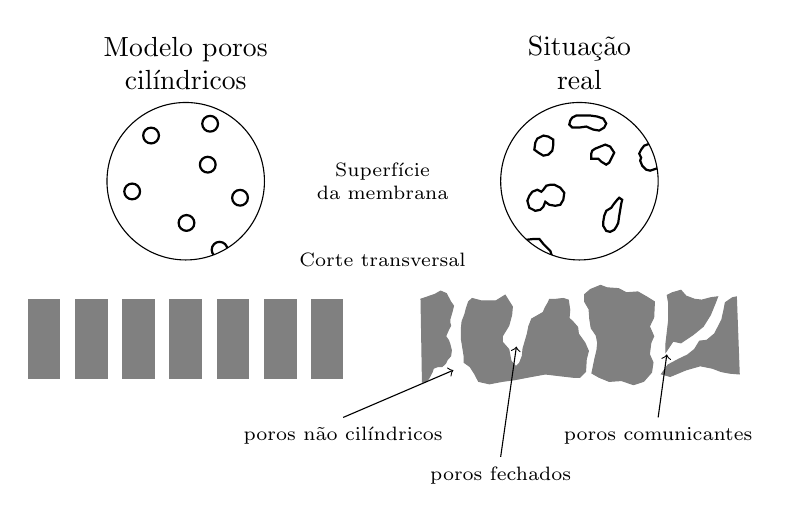
\begin{tikzpicture}

%\shade[left color=black!3!white, right color=black!5!white] (-1,-1) rectangle (12,10);
%\draw[help lines] (0,-1) grid (11,6);

\filldraw[gray] (1,2) -- (1.4,2) -- (1.4,1) -- (1,1);
\filldraw[gray] (5,2) -- (4.6,2) -- (4.6,1) -- (5,1);
\foreach \x in {1.6,2.2,2.8,3.4,4}
	{
		\filldraw[gray] (\x,1) rectangle (\x+0.4,2);
	}

\filldraw[gray] (5.981776765,2)--
(6.072892938,2.03125)--
(6.164009112,2.0625)--
(6.23690205,2.104166667)--
(6.309794989,2.072916667)--
(6.364464692,1.96875)--
(6.400911162,1.916666667)--
(6.382687927,1.84375)--
(6.355353075,1.75)--
(6.355353075,1.697916667)--
(6.364464692,1.666666667)--
(6.337129841,1.614583333)--
(6.318906606,1.572916667)--
(6.300683371,1.53125)--
(6.337129841,1.479166667)--
(6.355353075,1.427083333)--
(6.37357631,1.354166667)--
(6.364464692,1.28125)--
(6.318906606,1.229166667)--
(6.300683371,1.1875)--
(6.255125285,1.145833333)--
(6.200455581,1.145833333)--
(6.145785877,1.125)--
(6.127562642,1.072916667)--
(6.10022779,1.020833333)--
(6.082004556,0.989583333)--
(6.045558087,0.947916667)--
(6,0.947916667);

\filldraw[gray]
(6.6378,	2.0104)--
(6.5923,	1.9688)--
(6.5649,	1.8854)--
(6.5467,	1.8125)--
(6.5103,	1.7188)--
(6.5011,	1.6250)--
(6.5011,	1.5000)--
(6.5194,	1.3854)--
(6.5376,	1.2708)--
(6.5376,	1.1979)--
(6.6105,	1.1458)--
(6.6651,	1.0625)--
(6.7198,	0.9583)--
(6.8565,	0.9271)--
(7.0205,	0.9583)--
(7.1754,	0.9792)--
(7.3941,	1.0208)--
(7.5672,	1.0521)--
(7.7403,	1.0313)--
(7.9226,	1.0104)--
(8.0046,	1.0104)--
(8.0774,	1.0833)--
(8.0866,	1.2396)--
(8.1139,	1.3438)--
(8.0683,	1.4479)--
(7.9863,	1.5625)--
(7.9772,	1.6458)--
(7.9134,	1.7188)--
(7.8679,	1.7604)--
(7.8770,	1.8646)--
(7.8588,	1.9896)--
(7.7950,	2.0104)--
(7.7039,	2.0000)--
(7.6219,	2.0000)--
(7.6036,	1.9583)--
(7.5672,	1.8958)--
(7.5399,	1.8333)--
(7.4670,	1.7917)--
(7.3941,	1.7500)--
(7.3576,	1.6563)--
(7.3394,	1.5625)--
(7.3121,	1.4688)--
(7.2847,	1.3750)--
(7.2756,	1.2813)--
(7.2392,	1.1875)--
(7.1936,	1.1458)--
(7.1298,	1.2188)--
(7.1025,	1.3646)--
(7.0205,	1.4583)--
(7.0205,	1.5313)--
(7.1025,	1.6667)--
(7.1390,	1.8021)--
(7.1481,	1.9063)--
(7.0569,	2.0521)--
(6.9385,	1.9792)--
(6.7563,	1.9792)--cycle;

\filldraw[gray]
(8.0683,2.0625)--
(8.0683,1.9688)--
(8.1230,1.8750)--
(8.1321,1.7500)--
(8.1503,1.6354)--
(8.2141,1.5417)--
(8.2323,1.4479)--
(8.2232,1.3542)--
(8.1959,1.2396)--
(8.1595,1.0625)--
(8.2506,1.0104)--
(8.3781,0.9583)--
(8.5330,0.9688)--
(8.6879,0.9167)--
(8.8155,0.9583)--
(8.9157,1.0729)--
(8.9339,1.1979)--
(8.8884,1.3021)--
(8.9066,1.4479)--
(8.9431,1.5313)--
(8.8884,1.6563)--
(8.9431,1.7708)--
(8.9522,1.9688)--
(8.8519,2.0313)--
(8.7426,2.0938)--
(8.5968,2.0833)--
(8.4966,2.1354)--
(8.3508,2.1458)--
(8.2688,2.1771)--
(8.1412,2.1250)--cycle;

\filldraw[gray]
(9.1162,2.0521)--
(9.1344,1.9479)--
(9.1344,1.7396)--
(9.1162,1.5833)--
(9.0979,1.4271)--
(9.0979,1.3333)--
(9.1891,1.4688)--
(9.2893,1.4479)--
(9.4442,1.5521)--
(9.5718,1.6563)--
(9.6629,1.8021)--
(9.7267,1.9583)--
(9.7540,2.0313)--
(9.6720,2.0208)--
(9.5535,1.9896)--
(9.4624,2.0000)--
(9.3531,2.0417)--
(9.2893,2.1146)--
(9.1800,2.0833)--cycle;

\filldraw[gray]
(10.0000,2.0313)--
(9.9453,2.0208)--
(9.8542,1.9583)--
(9.8360,1.8646)--
(9.8087,1.7396)--
(9.7175,1.5625)--
(9.6173,1.4792)--
(9.5262,1.4688)--
(9.4624,1.3646)--
(9.3713,1.2917)--
(9.2620,1.2396)--
(9.1253,1.1667)--
(9.0433,1.0521)--
(9.1526,1.0208)--
(9.3531,1.1042)--
(9.5353,1.1563)--
(9.6902,1.1250)--
(9.7995,1.0833)--
(9.9089,1.0625)--
(10.0364,1.0521);





%
%\foreach \position in {(2.60,4.1),(2.57,3.46),(3.26,3.76),(3.51,3.22),(3,3)}
%		{
%			\draw[thick] \position circle (0.1cm);
%		}


%\draw[thick]
%(5.9694,3.7245)--
%(5.8914,3.6837)--
%(5.8357,3.6429)--
%(5.7911,3.6122)--
%(5.7688,3.5816)--
%(5.7688,3.5408)--
%(5.7799,3.5000)--
%(5.8245,3.4694)--
%(5.8914,3.4796)--
%(5.9582,3.5000)--
%(6.0251,3.5102)--
%(6.0919,3.4898)--
%(6.1699,3.4796)--
%(6.2256,3.4898)--
%(6.2702,3.5204)--
%(6.2925,3.5612)--
%(6.3036,3.6020)--
%(6.2702,3.6327)--
%(6.2479,3.6735)--
%(6.2033,3.6939)--
%(6.1476,3.7143)--
%(6.1031,3.7245)--
%(6.0474,3.7245)--cycle;
%\begin{scope}[xshift=0.5cm,yshift=-0.2cm]
%\draw[thick]
%(6.9053,3.8469)--
%(6.8719,3.8163)--
%(6.8384,3.7857)--
%(6.8050,3.7347)--
%(6.8050,3.6939)--
%(6.8496,3.6531)--
%(6.8942,3.6122)--
%(6.9721,3.6020)--
%(7.0390,3.6122)--
%(7.1058,3.6429)--
%(7.1838,3.6633)--
%(7.2396,3.7041)--
%(7.2507,3.7551)--
%(7.1950,3.7959)--
%(7.1393,3.8367)--
%(7.1058,3.8673)--
%(7.0390,3.8878)--
%(6.9944,3.8878)--
%(6.9499,3.8673)--cycle;
%\end{scope}
%\begin{scope}[xshift=1.2cm,yshift=-0.4cm]
%\draw[thick]
%(6.6825,3.2653)--
%(6.6490,3.2245)--
%(6.6045,3.1837)--
%(6.5710,3.1531)--
%(6.6045,3.1122)--
%(6.6713,3.1122)--
%(6.7716,3.1429)--
%(6.8384,3.1633)--
%(6.9276,3.1837)--
%(7.0279,3.1939)--
%(7.1170,3.1735)--
%(7.2061,3.1939)--
%(7.2953,3.2347)--
%(7.3510,3.2857)--
%(7.3955,3.3265)--
%(7.4290,3.3776)--
%(7.4624,3.4286)--
%(7.4735,3.4796)--
%(7.4178,3.5204)--
%(7.3398,3.5306)--
%(7.2730,3.5204)--
%(7.2284,3.4796)--
%(7.1838,3.4490)--
%(7.1281,3.4184)--
%(7.0836,3.3776)--
%(7.0279,3.3776)--
%(6.9833,3.3571)--
%(6.9276,3.3469)--
%(6.8607,3.3469)--
%(6.8050,3.3367)--
%(6.7493,3.3163)--
%(6.7159,3.2857)--cycle;
%\end{scope}
%\begin{scope}[xshift=0cm,yshift=0.5cm]
%\draw[thick]
%(8.2423,3.7857)--
%(8.1309,3.7551)--
%(8.0529,3.7245)--
%(7.9972,3.6735)--
%(7.9638,3.6224)--
%(7.9415,3.5714)--
%(7.9526,3.5000)--
%(7.9749,3.4184)--
%(7.9972,3.3776)--
%(8.0752,3.3367)--
%(8.1532,3.3061)--
%(8.2201,3.3367)--
%(8.2646,3.3571)--
%(8.2869,3.2959)--
%(8.3426,3.2449)--
%(8.4095,3.2143)--
%(8.4763,3.1837)--
%(8.5766,3.1735)--
%(8.6657,3.1837)--
%(8.7103,3.2347)--
%(8.7660,3.2857)--
%(8.7883,3.3469)--
%(8.7994,3.4184)--
%(8.7772,3.5000)--
%(8.7214,3.5510)--
%(8.6435,3.5816)--
%(8.5543,3.5816)--
%(8.4875,3.5714)--
%(8.4095,3.5408)--
%(8.4095,3.6020)--
%(8.3872,3.6837)--
%(8.3538,3.7347)--
%(8.3092,3.7653)--cycle;
%\end{scope}
%
%\begin{scope}[xshift=2.3cm,yshift=2.6cm]
%\draw[clip] (0.7,0.9) circle (1cm);
%\foreach \position in {(0,0.4),(0,1.2),(0,2),(0.4,0),(0.4,0.8),(0.4,1.6),(0.8,0.4),(0.8,1.2),(0.8,2)%
%	,(1.2,0),(1.2,0.8),(1.2,1.6),(1.6,0.4),(1.6,1.2),(1.6,2),(2,0),(2,0.8),(2,1.6)}
%	\draw[thick] \position circle (0.1cm);
%\end{scope}
%%\draw[thick] (1,3)--(5,3) (1,4)--(5,4) (6,3)--(10,3) (6,4)--(10,4);
%%\draw (3,3.5) circle (1cm);
%%\begin{scope}[xshift=2.3cm,yshift=2.6cm]
%%\foreach \position in {(0,0.4),(0,1.2),(0,2),(0.4,0),(0.4,0.8),(0.4,1.6),(0.8,0.4),(0.8,1.2),(0.8,2)%
%%	,(1.2,0),(1.2,0.8),(1.2,1.6),(1.6,0.4),(1.6,1.2),(1.6,2),(2,0),(2,0.8),(2,1.6)}
%%	\draw[thick] \position circle (0.1cm);
%%\end{scope}
%\draw (8,3.5) circle (1cm);
%
%\draw (3,6) circle (1cm);
%\draw (8,6) circle (1cm);
\begin{scope}
\draw[clip] (3,3.5) circle (1cm);
\foreach \position in {(2.32,3.37),(2.56,4.08),(3.31,4.23),(3.28,3.71),(3.01,2.97),(3.43,2.63),(3.69,3.29)}
	\draw[thick] \position circle (0.1cm);
\end{scope}

\begin{scope}
\draw[clip] (8,3.5)circle(1cm);
\draw[thick]
(7.5163,3.3662)--
(7.4656,3.3917)--
(7.4022,3.3662)--
(7.3641,3.3153)--
(7.3388,3.2516)--
(7.3641,3.1624)--
(7.4402,3.1242)--
(7.5036,3.1369)--
(7.5417,3.1752)--
(7.5670,3.2389)--
(7.6178,3.2006)--
(7.6938,3.1879)--
(7.7572,3.2006)--
(7.7953,3.2643)--
(7.8080,3.3535)--
(7.7572,3.4172)--
(7.6812,3.4554)--
(7.6304,3.4554)--
(7.5797,3.4427)--
(7.5417,3.3917)--cycle;
\draw[thick]
(8.3025,2.9841)--
(8.3152,3.0605)--
(8.3406,3.1242)--
(8.4040,3.1624)--
(8.4293,3.2006)--
(8.4801,3.2643)--
(8.5054,3.2898)--
(8.5435,3.2643)--
(8.5308,3.2134)--
(8.5181,3.1369)--
(8.5054,3.0605)--
(8.4928,2.9713)--
(8.4674,2.9204)--
(8.4420,2.8822)--
(8.3913,2.8567)--
(8.3406,2.8694)--
(8.3025,2.9331)--cycle;
\draw[thick]
(8.1630,3.8885)--
(8.1504,3.8503)--
(8.1504,3.7866)--
(8.1884,3.7866)--
(8.2391,3.7866)--
(8.2772,3.7484)--
(8.3406,3.7102)--
(8.3786,3.7357)--
(8.4167,3.8121)--
(8.4420,3.8631)--
(8.3913,3.9395)--
(8.3279,3.9650)--
(8.2645,3.9395)--
(8.2011,3.9140)--cycle;
\draw[thick]
(7.4656,4.0414)--
(7.4402,3.9904)--
(7.4275,3.9013)--
(7.4783,3.8631)--
(7.5417,3.8248)--
(7.6051,3.8376)--
(7.6558,3.8885)--
(7.6685,3.9650)--
(7.6685,4.0287)--
(7.6051,4.0669)--
(7.5417,4.0796)--
(7.5163,4.0669)--cycle;
\draw[thick]
(7.9094,4.3089)--
(7.8841,4.2707)--
(7.8714,4.2197)--
(7.9094,4.1815)--
(7.9982,4.1815)--
(8.0870,4.1943)--
(8.1757,4.1561)--
(8.2518,4.1433)--
(8.3152,4.1815)--
(8.3406,4.2325)--
(8.3025,4.2962)--
(8.2264,4.3217)--
(8.1377,4.3344)--
(8.0109,4.3344)--
(7.9601,4.3344)--cycle;
\draw[thick]
(7.1993,2.7420)--
(7.3134,2.7548)--
(7.4275,2.7675)--
(7.4909,2.7675)--
(7.5417,2.7038)--
(7.5924,2.6529)--
(7.6304,2.6146)--
(7.6558,2.5382)--
(7.6431,2.4236);
\draw[thick]
(8.9746,3.9777)--
(8.8986,3.9777)--
(8.8225,3.9522)--
(8.7844,3.9013)--
(8.7591,3.8503)--
(8.7844,3.7994)--
(8.7717,3.7611)--
(8.7971,3.6975)--
(8.8478,3.6465)--
(8.8986,3.6338)--
(8.9746,3.6592)--
(9.0507,3.6847)--
(9.1014,3.7357);
\end{scope}

\node[align=center,font=\scriptsize] at (5.5,3.5) {Superfície\\ da membrana};
\node[font=\scriptsize] at (5.5,2.5) {Corte transversal};

\node[align=center] at (3,5) {Modelo poros\\cilíndricos};
\node[align=center] at (8,5) {Situação \\ real};

\node[below,font=\scriptsize] at (5,0.5) {poros não cilíndricos};
\node[below,font=\scriptsize] at (7,0) {poros fechados};
\node[below,font=\scriptsize] at (9,0.5) {poros comunicantes};
\draw[->] (5,0.5) -- (6.4,1.1);
\draw[->] (7,0) -- (7.2,1.4);
\draw[->] (9,0.5) -- (9.11,1.3);




\end{tikzpicture}
	\caption[Desvio ao modelo de poros cilíndricos]{Ilustração do desvio ao modelo ideal de poros cilíndricos apresentado por membranas de MF e UF\@. A estrutura de uma membrana real pode diferir significativamente da situação ideal, por exemplo contendo poros não cilíndricos, poros fechados e poros comunicantes.}
	\label{fig:mpcilindricos}
\end{figure}

O desenvolvimento teórico descrito neste capítulo é assim baseado no modelo dos poros cilíndricos. Considera-se igualmente que os coeficientes de transferência de massa, muito dependentes da geometria do módulo de membranas utilizado, são conhecidos ou podem ser determinados experimentalmente.

\section{Permeabilidade de membranas de MF e UF} % (fold)
\label{sec:teo1}
\index{ultrafiltração!permeabilidade}
\index{microfiltração!permeabilidade}
As membranas de MF e UF são consideradas membranas porosas, isto é, na sua estrutura existem poros de pequenas dimensões por onde ocorre, na sua totalidade, o transporte de massa. Excluídos deste processo de transferência de massa estão os solutos cujas dimensões e/ou carga elétrica não lhes permitam permear através desta estrutura porosa. Se os poros forem considerados cilíndricos, o fluxo de líquido pode ser relacionado com o diferencial de pressão ao longo da membrana através de um simples balanço de quantidade de movimento. Se o escoamento através de um poro cilíndrico, perpendicular à superfície da membrana, for laminar (como é geralmente o caso em processos de MF e UF), e estiver completamente desenvolvido, o perfil de velocidade é função da coordenada radial adimensional, \radialadimensional ($=r/\raioporo$) \cite{bird}:\index{coordenadas!radial adimensional}
\begin{equation}
 	\label{eq:bird}
 	v(\radialadimensional)=2\fluxoporo(1-\radialadimensional^2)
 \end{equation}
\index{velocidade!fluido num poro} 
onde $v$ é a velocidade do líquido (função de \radialadimensional) e \fluxoporo\ é o fluxo de líquido no poro dado por:
\begin{equation}
	\label{eq:fluxoporo}
	\fluxoporo=\frac{\raioporo^2}{8\viscosidade\comporo}\Delta p
\end{equation}
\index{equação!Hagen-Poiseuille}\index{fluxo!poro}%
onde $\Delta p$ representa o diferencial de pressão ao longo do poro, \raioporo\ o raio do poro, \viscosidade\ a viscosidade e \comporo\ o comprimento do poro. A equação~\ref{eq:fluxoporo} é conhecida como a equação de Hagen-Poiseuille, e um escoamento que obedeça à referida equação é denominado como um escoamento de Poiseuille.\index{Hagen-Poiseuille} 
Uma quantidade de maior interesse em processos de MF e UF é o caudal de filtração por unidade de área de membrana, \fluxo, normalmente denominado fluxo de filtração. Considerando que a membrana contém $n_p$ poros cilíndricos paralelos, todos com raio \raioporo, então \fluxo\ é dado por:\index{fluxo!filtração}
\begin{equation}
\begin{aligned}
	\label{eq:fluxopoise}
	\caudal &=\fluxo\areamembrana = \fluxoporo n_p\pi\raioporo^2 \\
     \fluxo&=\porosidade\fluxoporo
\end{aligned}
\end{equation}\index{area@área!membrana}%
onde \caudal\ é o caudal (volumétrico) de filtração, \areamembrana\ é a área total da superfície da membrana e \porosidade\ é a fração da área total de membrana ocupada pelos poros, denominada porosidade ($\porosidade=n_p\pi\raioporo^2/\areamembrana$).\index{porosidade}\index{caudal volumétrico} 
Assim, pelas equações~\ref{eq:fluxoporo}~e~\ref{eq:fluxopoise}, o fluxo de filtração é dado por:
\begin{equation}
 	\label{eq:fluxopoisec}
 	\fluxo=\frac{\porosidade\raioporo^2}{8\viscosidade\comporo}\Delta p
\end{equation} 
A equação~\ref{eq:fluxopoisec} pode ainda ser modificada pela inclusão de um parâmetro \tortuosidade\ (tortuosidade) que possa contabilizar o afastamento à situação ideal de se terem poros perpendiculares à superfície da membrana \cite{mulder}.\index{tortuosidade}
Assim, se o comprimento médio dos poros numa situação não ideal for $\overline{\comporo}$ e a espessura da membrana for \commembrana, o parâmetro tortuosidade é definido como $\tortuosidade=\overline{\comporo}/\commembrana$, e a equação~\ref{eq:fluxopoisec} vem assim:
\begin{equation}
	\label{eq:poisemod}
	\fluxo=\frac{\porosidade\raioporo^2}{8\viscosidade\tortuosidade\commembrana}\Delta p
\end{equation}
É importante notar que o parâmetro \tortuosidade\ deve ser visto como um parâmetro empírico, uma vez que a equação~\ref{eq:bird} só é válida para poros paralelos à direção do escoamento. A equação~\ref{eq:poisemod} indica que o fluxo de líquido através da membrana é diretamente proporcional ao diferencial de pressão. Com exceção da viscosidade, a constante de proporcionalidade é apenas função de características intrínsecas da membrana e é designada por permeabilidade hidráulica (\permhidra).\index{permeabilidade hidráulica} 
Assim a equação~\ref{eq:poisemod} pode ser reescrita da seguinte forma \cite{latu09}:
\begin{equation}
	\label{eq:permhidro}
	\fluxo=\permhidra\Delta p
\end{equation}
A permeabilidade hidráulica é uma característica específica de cada membrana e a sua determinação permite aferir o grau de colmatação. Importa também salientar que durante a filtração de soluções que contenham solutos que sejam parcialmente (ou totalmente) retidos pela membrana, a relação linear entre o fluxo de filtração e a pressão aplicada não é verificada experimentalmente, o que se deve em parte à ocorrência de um aumento de concentração destes solutos junto à membrana, um fenómeno conhecido como polarização de concentração, discutido na secção~\ref{sec:filmepol}. 
% section teo1 (end)

\section{Equações de Maxwell-Stefan}
\label{sec:ems}\index{Maxwell-Stefan}
O transporte de massa em processos de MF e UF pode ser descrito segundo várias abordagens. Uma abordagem possível é através das equações de Maxwell-Stefan (MS). Uma descrição pormenorizada destas equações pode ser encontrada na literatura \cite{wesslivro,krishna,noordman,taylor}. Em termos qualitativos, as equações de MS indicam que, em condições de estado estacionário, a força motriz aplicada num componente de uma mistura é contrabalançada pela força de atrito provocada pelo movimento relativo deste componente na mistura. Para um dado componente $i$ numa mistura de vários componentes $j$ as equações de MS assumem a seguinte forma (ver igualmente a figura~\ref{fig:MSteste}):
\begin{figure}
\centering
%!TEX root=testfigum.tex
\begin{tikzpicture}
%\draw[help lines] (0,0) grid (10,4);
\node[font=\large] at (5,2) {$\displaystyle \vec{F}_i=\sum_{j\neq i}\atrito_{i,j}x_j(\vec{u}_i-\vec{u}_j)$};
\node[below, align=center] at (1,1) {Força motriz\\no componente $i$};
\draw[->] (1,1) -- (2.9,1.9);
\node[above, align=center] at (3,3) {Coeficiente de atrito\\entre $i$ e $j$};
\draw[->] (4,3) -- (4.6,2.5);
\node[below, align=center] at (4.25,1) {Fração molar\\do componente $j$};
\draw[->] (4.25,1) -- (5.1,1.9);
\node[above, align=center] at (8,3) {Velocidade do componente $i$\\(difusiva)};
\draw[->] (7,3) -- (5.95,2.45);
\node[below, align=center] at (8,1) {Velocidade do componente $j$\\(difusiva)};
\draw[->] (8,1) -- (6.9,1.9);
\end{tikzpicture}
\caption{Equações de Maxwell-Stefan.}
\label{fig:MSteste}
\end{figure}
\begin{equation}
	\label{eq:ms1}
	\vec{F_{i}}=\sum_{j\neq i} \atrito_{i,j}x_{j}(\vec{u_{i}}-\vec{u_{j}})
\end{equation}
\index{equação!Maxwell-Stefan}%
onde $\vec{F_{i}}$ é a força motriz por mole do componente $i$, $\atrito_{i,j}$ é o coeficiente de atrito molar entre $i$ e $j$, $x_{j}$ é a fração molar de $j$, $\vec{u_{i}}$ é a velocidade do componente $i$ e $\vec{u_{j}}$ a velocidade do componente $j$. As velocidades que figuram na equação~\ref{eq:ms1} são velocidades difusivas. Para além da velocidade difusiva, um componente pode ter igualmente uma velocidade convectiva ($\vec{v}$) provocada pelo movimento da mistura como um todo. Assim, a velocidade total, $\vec{w}$, de um determinado componente $i$ de uma mistura é dada pela soma destas duas velocidades:\index{velocidade!difusiva}\index{velocidade!convectiva}\index{velocidade!total}
\begin{equation}
	\label{eq:veltotal}
	\vec{w}_{i}=\vec{u}_{i}+\vec{v}_{i}
\end{equation}
A força motriz $\vec{F}_{i}$ é dada pelo simétrico do gradiente de um potencial (\potencialms):
\begin{equation}
 	\label{eq:mspot}
 	-\nabla\potencialms_i=\sum_{j\neq i} \atrito_{i,j}x_{j}(\vec{u_{i}}-\vec{u_{j}})
 \end{equation}\index{potencial!Maxwell-Stefan}%
O potencial que figura na equação~\ref{eq:mspot} representa a soma dos vários potenciais referentes ao componente $i$, como por exemplo o potencial gravítico, centrífugo ou eletroquímico, sendo este último o único com interesse no presente trabalho. O potencial eletroquímico de um dado componente $i$ é dado por \cite{bowen02}:
\begin{equation}
\label{eq:potq}
\potqui_{i}=\ctegases T\ln\atividade_{i} + \cargaeletrica_{i}\ctefaraday\potencial + V_{i}p + \mathrm{constante} 	
\end{equation}\index{potencial!eletroquímico}\index{volume!parcial molar}% 
onde $\potqui_{i}$ é o potencial eletroquímico da espécie $i$, \ctegases\ é a constante dos gases perfeitos, $T$ é a temperatura absoluta, $\atividade_{i}$ é a atividade, $\cargaeletrica_{i}$ é a valência elétrica, \ctefaraday\ é a constante de Faraday, \potencial\ o potencial elétrico, $V_{i}$ o volume parcial molar e $p$ a pressão. A força motriz é assim dada pelo gradiente espacial do potencial eletroquímico, o que para uma situação de transporte de massa unidimensional, segundo uma coordenada $y$, resulta em:
\begin{equation}
	\label{eq:formo}
	F_{i}=-\frac{d\potqui_{i}}{dy}=-\left(\ctegases T\frac{d\ln \atividade_{i}}{dy}+\cargaeletrica_{i}\ctefaraday\frac{d\potencial}{dy}+V_{i}\frac{dp}{dy}\right)
\end{equation}
A dependência do potencial eletroquímico com a pressão pode ser importante, em especial quando o volume molar do componente é elevado. No entanto é por vezes desprezada tendo em conta a maior dependência com a atividade e potencial elétrico. No presente trabalho opta-se por desprezar o termo referente à pressão para simplificar um pouco a formulação das equações e agilizar os cálculos inerentes.

As equações de MS representadas na equação~\ref{eq:mspot} podem ser enormemente simplificadas considerando algumas aproximações.\index{solução!diluída} Em primeiro lugar, assumindo que as soluções são diluídas e ideais, as atividades dos componentes são iguais às suas frações molares. 
\index{Maxwell-Stefan!simplificações da equação}
Por outro lado, sendo soluções diluídas, assume-se que a força de atrito sobre um soluto $i$ da solução, dada pelo segundo membro da equação~\ref{eq:mspot}, é aproximadamente igual à força de atrito resultante do seu movimento relativo em relação ao solvente. A justificação para esta aproximação passa por verificar que a força de atrito entre solutos é proporcional à fração molar dos mesmos, frações molares estas, que para o caso de soluções diluídas assumem valores reduzidos (ver figura~\ref{fig:soldil}). Por fim, assume-se que o transporte de massa pode ser aproximadamente descrito por uma abordagem unidimensional segundo uma coordenada $y$. Assim, as equações de MS assumem a seguinte forma simplificada:
\begin{equation}
  	\label{eq:mssim}
  	-\left(\ctegases T\frac{d\ln x_{i}}{dy}+\cargaeletrica_{i}\ctefaraday\frac{d\potencial}{dy}\right)=\atrito_{i,w}x_{w}(u_{i}-u_{w})
\end{equation}
\begin{figure}[t]
\centering
%!TEX root=testfigum.tex
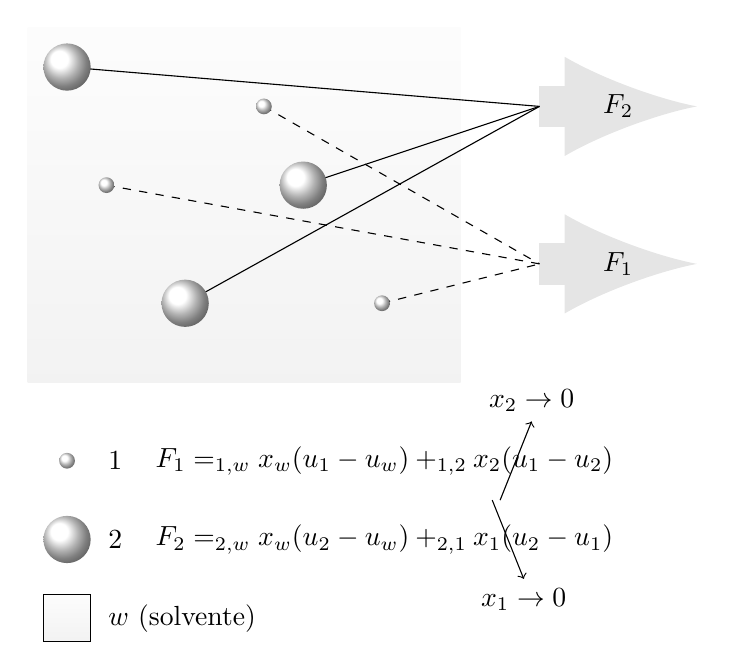
\begin{tikzpicture}

%\draw[help lines] (0,0) grid (10,8);

\shadedraw[thin,bottom color=black!5!white, top color=black!1!white] (0.7,-0.3) rectangle (1.3,0.3);
\node[right] at (1.4,0) {$w$ (solvente)};
\shade[bottom color=black!5!white, top color=black!1!white] (0.5,3) rectangle (6,7.5);
%\fill[black!5!white] (0.5,3) rectangle (6,7.5);

\coordinate (a) at (7,6.5);
\coordinate (b) at (9,6.5);
\draw[->, >=latex,black!10!white, line width=15pt]   (a) to node[black]{$F_2$} (b) ;

\coordinate (c) at (7,4.5);
\coordinate (d) at (9,4.5);
\draw[->, >=latex,black!10!white, line width=15pt]   (c) to node[black]{$F_1$} (d) ;

\shade [ball color=white] (1,2) circle [radius=0.1cm];
\node[right] at (1.4,2) {1};
\node[right] at (2,2) {$F_1=\atrito_{1,w}x_w(u_1-u_w)+\atrito_{1,2}x_2(u_1-u_2)$};
\draw[->] (6.5,1.5)--(6.9,2.5) node[above] {$x_2\rightarrow 0$};

\shade [ball color=white] (1,1) circle [radius=0.3cm];
\node[right] at (1.4,1) {2};
\node[right] at (2,1) {$F_2=\atrito_{2,w}x_w(u_2-u_w)+\atrito_{2,1}x_1(u_2-u_1)$};
\draw[->] (6.4,1.5)--(6.8,0.5) node[below] {$x_1\rightarrow 0$};

\draw[thin] (1,7) -- (a);
\draw[thin] (2.5,4) -- (a);
\draw[thin] (4,5.5) -- (a);

\begin{scope}[dashed]
\draw[thin] (1.5,5.5) -- (c);
\draw[thin] (3.5,6.5) -- (c);
\draw[thin] (5,4) -- (c);
\end{scope}

\shade [ball color=white] (1,7) circle [radius=0.3cm];
\shade [ball color=white] (2.5,4) circle [radius=0.3cm];
\shade [ball color=white] (4,5.5) circle [radius=0.3cm];

\shade [ball color=white] (1.5,5.5) circle [radius=0.1cm];
\shade [ball color=white] (3.5,6.5) circle [radius=0.1cm];
\shade [ball color=white] (5,4) circle [radius=0.1cm];



%\node[left] at (1,2) {$F_i=\atrito_{1,w}$};


\end{tikzpicture}
\caption[Representação de uma solução diluída de dois solutos]{Representação de uma solução diluída de dois solutos (1 e 2) num solvente ($w$). Para soluções diluídas, as forças de atrito entre solutos podem ser desprezadas devido às reduzidas frações molares dos mesmos.}
\label{fig:soldil}
\end{figure}%
O índice $w$ é usado para indicar que a propriedade se refere ao solvente, que no caso deste trabalho é a água. A equação~\ref{eq:mssim} pode ainda ser simplificada considerando que, como as soluções são diluídas, $x_{w}\approx 1$. Por outro lado, assume-se que a velocidade difusiva do solvente é nula $u_w\approx 0$. Esta suposição está de acordo com a opção de se escolher a velocidade do solvente como velocidade de referência, discutida por Taylor e Krishna \cite{taylor}. Assim, tendo em conta a equação~\ref{eq:veltotal}, obtém-se por fim:
\begin{equation}
	\label{eq:mssimples}
	-\left(\ctegases T\frac{d\ln x_{i}}{dy}+\cargaeletrica_{i}\ctefaraday\frac{d\potencial}{dy}\right)=\atrito_{i,w}(w_{i}-v_{i})
\end{equation}
A velocidade convectiva do componente $i$ ($v_{i}$) nem sempre assume o mesmo valor da velocidade convectiva do solvente, em especial quando a solução se encontra confinada como é o caso na permeação através de poros de membranas. No entanto as duas velocidades são proporcionais, sendo a constante de proporcionalidade denominada seletividade convectiva ($\alpha_i$) \cite{noordman}:
\index{seletividade!convectiva}
\begin{equation}
 	\label{eq:alfa}
 	v_i=\alpha_i v_w
 \end{equation} 
Na secção~\ref{sec:restringido} será abordada uma situação em que $\alpha_i$ é diferente de 1. Pode-se ainda referir que o coeficiente de atrito, \atrito, pode ser facilmente relacionado com o coeficiente de difusão, $D$, através da seguinte equação \cite{wesslivro,taylor,krishna}\index{coeficiente!de atrito molar}
\index{coeficiente!de difusão}
\footnote{A grande maioria dos valores do coeficiente de difusão de solutos reportados na literatura são coeficientes de difusão de Fick. Em condições não ideais, o coeficiente de difusão de Fick não é igual ao coeficiente de difusão que figura nas equações de MS \cite{wesslivro}. No entanto, no âmbito deste trabalho assume-se que os dois coeficientes são iguais, como resultado de se considerarem as soluções como ideais.}:
\begin{equation}
	\label{eq:DeA}
	\atrito=\frac{RT}{D}
\end{equation} 

Uma primeira aplicação da equação~\ref{eq:mssimples}, que serve simultaneamente como exemplo, é a dedução da equação de Stokes-Einstein. Para isso, considera-se uma solução não confinada, diluída e ideal, de um soluto com dimensões suficientemente superiores às do solvente para que o seja possível tratar como uma partícula hidrodinâmica. Considera-se que existe um gradiente de concentração do soluto, que se assume unidimensional segundo $y$, e que a solução se encontra em repouso, o que resulta numa velocidade convectiva de soluto nula\footnote{Não é necessário supor que o gradiente de concentração do soluto é unidimensional para efetuar a presente dedução. O resultado obtido será o mesmo considerando o gradiente tridimensional.}. Nestas condições, considerando que o soluto é neutro ($\cargaeletrica=0$), a equação~\ref{eq:mssimples} pode ser escrita na seguinte forma:
\begin{equation}
 	\label{eq:dedse1}
 	-\ctegases T\frac{d\ln x}{dy}=\atrito u
 \end{equation} 
Note-se que como a velocidade convectiva do soluto é nula, a velocidade total é igual à velocidade difusiva. Multiplicando ambos os membros da equação pela concentração do soluto, $x\conctotal$, em que \conctotal\ é a concentração molar total da solução, obtém-se:
\begin{equation}
	\label{eq:dedse2}
	-\ctegases T\frac{dC}{dy}=\atrito J
\end{equation}
onde $J$ é o fluxo difusivo molar de soluto ($J=x\conctotal u$). Se o soluto for considerado esférico, o coeficiente de atrito pode ser obtido pela lei de Stokes (figura~\ref{fig:MSstokes}):
\begin{figure}
\centering
%!TEX root=testfigum.tex
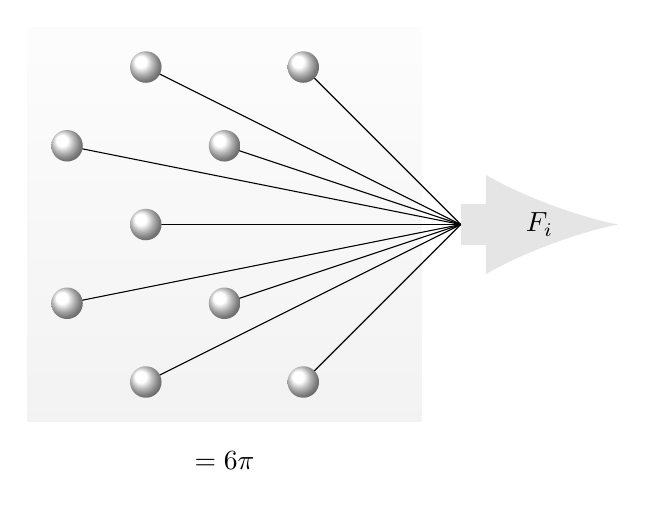
\begin{tikzpicture}

%\draw[help lines] (0,0) grid (10,8);

%\fill[black!5!white] (1.5,1.5) rectangle (6.5,6.5);
\shade[bottom color=black!5!white, top color=black!1!white] (1.5,1.5) rectangle (6.5,6.5);

\coordinate (a) at (7,4);
\coordinate (b) at (9,4);
\draw[->, >=latex,black!10!white, line width=15pt]   (a) to node[black]{$F_i$} (b) ;

\draw[thin] (3,6) -- (7,4);
\draw[thin] (3,2) -- (7,4);
\draw[thin] (2,5) -- (7,4);
\draw[thin] (2,3) -- (7,4);
\draw[thin] (4,5) -- (7,4);
\draw[thin] (4,3) -- (7,4);
\draw[thin] (5,2) -- (7,4);
\draw[thin] (3,4) -- (7,4);
\draw[thin] (5,6) -- (7,4);

\shade [ball color=white] (3,6) circle [radius=0.2cm];
\shade [ball color=white] (3,2) circle [radius=0.2cm];
\shade [ball color=white] (2,5) circle [radius=0.2cm];
\shade [ball color=white] (2,3) circle [radius=0.2cm];
\shade [ball color=white] (4,5) circle [radius=0.2cm];
\shade [ball color=white] (4,3) circle [radius=0.2cm];
\shade [ball color=white] (5,2) circle [radius=0.2cm];
\shade [ball color=white] (3,4) circle [radius=0.2cm];
\shade [ball color=white] (5,6) circle [radius=0.2cm];

\node at (4,1) {$\atrito=6\pi\viscosidade\raiostokes\avogadro$};

\end{tikzpicture}
\caption[Coeficiente de atrito para uma solução de um soluto esférico]{Ilustração do coeficiente de atrito para uma solução de um soluto esférico. A força de atrito por mol de soluto é igual à força de atrito de uma molécula (esférica), dada pela lei de Stokes, multiplicada pela número de Avogadro.}
\label{fig:MSstokes}
\end{figure}
\begin{equation}
	\label{eq:leistokes}
	\atrito=6\pi\viscosidade\raiostokes\avogadro
\end{equation}
onde \raiostokes\ é o raio do soluto e \avogadro\ é o número de Avogadro. Assim, a equação~\ref{eq:dedse2}, após inclusão da equação~\ref{eq:leistokes}, resulta em:
\begin{equation}
	\label{eq:dedse3}
	\frac{\boltzman T}{6\pi\viscosidade\raiostokes}=\frac{-J}{dC/dy}
\end{equation}
O segundo membro da equação anterior não é mais que o coeficiente de difusão do soluto ($D$) pela primeira lei de Fick, obtendo-se assim a equação de Stokes-Einstein:\index{equação!Stokes-Einstein}
\begin{equation}
	\label{eq:stokesein}
	D=\frac{\boltzman T}{6\pi\viscosidade\raiostokes}
\end{equation}
Esta equação é importante no âmbito do presente trabalho porque permite relacionar o coeficiente de difusão de um soluto com as suas dimensões, representadas por \raiostokes.\index{raio!hidrodinâmico} 
Para um dado soluto, este parâmetro pode ser visto como o raio de uma esfera com igual difusividade, e é denominado o raio hidrodinâmico. Uma conclusão importante a tirar da equação anterior é o facto do coeficiente de difusão de solutos ser inversamente proporcional às suas dimensões. 

O transporte de massa em operações com membranas é muito influenciado pelas condições hidrodinâmicas do escoamento, o que leva à necessidade de formular um modelo hidrodinâmico para permitir a aplicação das equações de MS. Na secção seguinte será abordado o modelo usado neste trabalho, o modelo do filme, sendo também discutido o fenómeno de polarização de concentração.  

\section{Polarização de concentração e modelo do filme} % (fold)
\label{sec:filmepol}\index{polarização de concentração}
O transporte de massa através de membranas de micro e ultrafiltração pode ser dividido em duas fases: o transporte de componentes até à superfície da membrana e o transporte de componentes através dos poros. No transporte de componentes até à superfície da membrana, a solução não se encontra confinada em espaços pequenos, e o transporte pode ser descrito pelas equações de Maxwell-Stefan (MS) apresentadas na secção~\ref{sec:ems}. O mesmo não se passa durante a permeação em poros de membranas, onde o confinamento da mistura produz efeitos quer ao nível da difusão, quer ao nível da convecção, tal como discutido na secção~\ref{sec:restringido}. Nesta secção será abordada a primeira etapa, em que se procura determinar o perfil de concentração dos vários componentes da solução a ser filtrada, desde o seio da solução até à superfície da membrana. Para isso é preciso aplicar as equações de transporte, o que é apenas possível se for definido um modelo hidrodinâmico. Uma possibilidade é o denominado modelo do filme (ver figura~\ref{fig:modfilme}). Neste modelo, assume-se que desde uma distância da membrana superior a um determinado valor $\delta$ existe turbulência no seio do líquido, o que impossibilita o desenvolvimento de gradientes de concentração.\index{espessura camada de polarização} 
Para distâncias inferiores a esse valor (para y entre 0 e $\delta$, ver figura~\ref{fig:modfilme}), assume-se que se forma um filme de líquido onde se localiza toda a resistência ao transporte de massa\footnote{Uma descrição elaborada do modelo do filme pode ser encontrada na literatura, por exemplo \cite{zydneyfilm,vasan}}.
\index{modelo!do filme}
\begin{figure}
\centering
%!TEX root=testfigumV2.tex
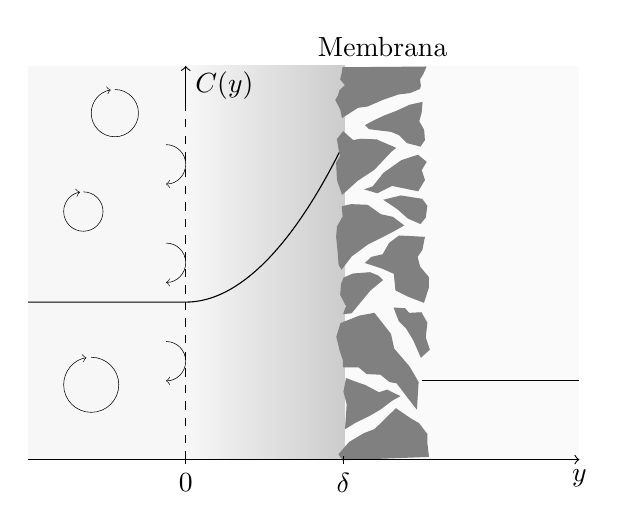
\begin{tikzpicture}

%\draw[help lines] (0,0) grid (12,7);

\fill[black!3!white] (2,1) rectangle (4,6);
\shade[left color=black!3!white, right color=black!20!white] (4,1) rectangle (6.02,6);
\fill[black!2!white] (6.02,1) rectangle (9,6);


\filldraw[gray] (6,5.983050847)--
(5.989690722,5.915254237)--
(5.969072165,5.830508475)--
(6.030927835,5.754237288)--
(5.958762887,5.686440678)--
(5.93814433,5.618644068)--
(5.907216495,5.56779661)--
(5.969072165,5.449152542)--
(5.989690722,5.347457627)--
(6.18556701,5.474576271)--
(6.309278351,5.491525424)--
(6.505154639,5.576271186)--
(6.701030928,5.644067797)--
(6.845360825,5.661016949)--
(6.969072165,5.711864407)--
(6.979381443,5.745762712)--
(6.969072165,5.830508475)--
(7.010309278,5.898305085)--
(7.051546392,5.991525424);
\filldraw[gray] (6.288659794,5.245762712)--
(6.329896907,5.203389831)--
(6.463917526,5.186440678)--
(6.608247423,5.169491525)--
(6.711340206,5.127118644)--
(6.81443299,5.025423729)--
(6.979381443,4.983050847)--
(7.030927835,5.059322034)--
(7.020618557,5.186440678)--
(6.958762887,5.296610169)--
(6.989690722,5.406779661)--
(7,5.533898305)--
(6.845360825,5.5)--
(6.680412371,5.423728814)--
(6.525773196,5.36440678)--
(6.381443299,5.296610169)--cycle;
\filldraw[gray] (6,5.161016949)--
(5.927835052,5.06779661)--
(5.948453608,4.940677966)--
(5.969072165,4.855932203)--
(5.917525773,4.771186441)--
(5.927835052,4.550847458)--
(5.989690722,4.372881356)--
(6.175257732,4.542372881)--
(6.391752577,4.686440678)--
(6.608247423,4.915254237)--
(6.659793814,4.957627119)--
(6.422680412,5.059322034)--
(6.226804124,5.06779661)--
(6.12371134,5.050847458)--cycle;
\filldraw[gray] (6.288659794,4.43220339)--
(6.432989691,4.389830508)--
(6.618556701,4.483050847)--
(6.824742268,4.440677966)--
(6.948453608,4.415254237)--
(7.030927835,4.550847458)--
(6.989690722,4.677966102)--
(7.051546392,4.779661017)--
(6.948453608,4.86440678)--
(6.742268041,4.796610169)--
(6.515463918,4.63559322)--
(6.381443299,4.466101695)--cycle;
\filldraw[gray] (5.989690722,4.211864407)--
(6,4.084745763)--
(5.927835052,3.957627119)--
(5.917525773,3.830508475)--
(5.93814433,3.618644068)--
(5.948453608,3.474576271)--
(5.979381443,3.423728814)--
(6.103092784,3.584745763)--
(6.309278351,3.737288136)--
(6.628865979,3.898305085)--
(6.762886598,3.974576271)--
(6.628865979,4.076271186)--
(6.474226804,4.110169492)--
(6.309278351,4.228813559)--
(6.103092784,4.237288136)--cycle;
\filldraw[gray] (6.288659794,3.5)--
(6.494845361,3.43220339)--
(6.649484536,3.36440678)--
(6.670103093,3.152542373)--
(6.824742268,3.076271186)--
(7.020618557,3)--
(7.082474227,3.186440678)--
(7.082474227,3.313559322)--
(6.969072165,3.449152542)--
(6.93814433,3.576271186)--
(7,3.669491525)--
(7.020618557,3.779661017)--
(7.030927835,3.822033898)--
(6.87628866,3.830508475)--
(6.711340206,3.838983051)--
(6.587628866,3.745762712)--
(6.505154639,3.601694915)--
(6.360824742,3.56779661)--cycle;
\filldraw[gray] (6.010309278,3.305084746)--
(5.979381443,3.228813559)--
(5.969072165,3.093220339)--
(6.041237113,2.949152542)--
(6.010309278,2.855932203)--
(6.103092784,2.86440678)--
(6.340206186,3.152542373)--
(6.494845361,3.279661017)--
(6.443298969,3.330508475)--
(6.340206186,3.372881356)--
(6.12371134,3.355932203)--cycle;
\begin{scope}[xshift=-0.08cm]
\filldraw[gray] (6.082474227,2.177966102)--
(6.082474227,2.262711864)--
(6.041237113,2.389830508)--
(6,2.559322034)--
(6.051546392,2.728813559)--
(6.288659794,2.822033898)--
(6.474226804,2.855932203)--
(6.680412371,2.593220339)--
(6.721649485,2.406779661)--
(6.917525773,2.177966102)--
(7.030927835,1.983050847)--
(7.010309278,1.652542373)--
(6.917525773,1.771186441)--
(6.762886598,1.974576271)--
(6.670103093,1.991525424)--
(6.556701031,2.084745763)--
(6.381443299,2.093220339)--
(6.278350515,2.177966102)--cycle;
\end{scope}

\filldraw[gray] (6.649484536,2.923728814)--
(6.711340206,2.762711864)--
(6.804123711,2.669491525)--
(6.896907216,2.516949153)--
(6.989690722,2.305084746)--
(7.092783505,2.398305085)--
(7.041237113,2.550847458)--
(7.06185567,2.737288136)--
(6.989690722,2.86440678)--
(6.835051546,2.855932203)--
(6.783505155,2.915254237)--cycle;
\filldraw[gray] (6.041237113,2.025423729)--
(6.010309278,1.86440678)--
(6.051546392,1.703389831)--
(6.030927835,1.398305085)--
(6.154639175,1.474576271)--
(6.329896907,1.559322034)--
(6.474226804,1.644067797)--
(6.618556701,1.754237288)--
(6.711340206,1.805084746)--
(6.556701031,1.881355932)--
(6.453608247,1.847457627)--
(6.278350515,1.940677966)--
(6.154639175,1.983050847)--cycle;
\filldraw[gray] (6,0.9915254237)--
(5.948453608,1.06779661)--
(6.082474227,1.220338983)--
(6.268041237,1.330508475)--
(6.402061856,1.381355932)--
(6.515463918,1.491525424)--
(6.670103093,1.644067797)--
(6.855670103,1.516949153)--
(6.958762887,1.457627119)--
(7.06185567,1.322033898)--
(7.06185567,1.211864407)--
(7.082474227,1.033898305);
\filldraw[gray] (6.525773196,4.296610169)--
(6.690721649,4.186440678)--
(6.824742268,4.06779661)--
(6.979381443,4)--
(7.041237113,4.076271186)--
(7.06185567,4.220338983)--
(7,4.305084746)--
(6.731958763,4.347457627)--cycle;

\begin{scope}[font=\normalsize]
\draw[dashed] (4,1) -- (4,6);
\draw[->] (2,1) -- (9,1);
\draw (4,0.95) -- (4,1.05);
\node[below] at (4,0.95) {0};
\draw (6,0.95) -- (6,1.05);
\node[below] at (6,0.95) {$\delta$};
\node[above] at (6.5,6) {Membrana};
\node[below] at (9,1) {$y$};
\draw (2,3)--(4,3)parabola(5.95,4.9);
\draw (7,2)--(9,2);
\node[above] at (8,2) {\concp};
\node[above] at (3,3) {\concb};
\node[left] at (5.95,4.9) {\concm};
\draw[->] (4,5.5)-- node[right] {$C(y)$}(4,6);
\draw[very thin,->] (3.75,2.5) arc [radius=0.25, start angle=90, end angle= -90];
\draw[very thin,->] (3.75,3.75) arc [radius=0.25, start angle=90, end angle= -90];
\draw[very thin,->] (3.75,5) arc [radius=0.25, start angle=90, end angle= -90];
\draw[very thin,->] (2.7,4.4) arc [radius=0.25, start angle=90, end angle=-260];
\draw[very thin,->] (2.8,2.3) arc [radius=0.35, start angle=90, end angle=-260];
\draw[very thin,->] (3.1,5.7) arc [radius=0.3, start angle=90, end angle=-260];
\end{scope}



%\begin{scope}[font=\scriptsize,scale=1.5]
%%\draw[fill=lightgray] (4,1) rectangle (5,4);
%\draw[dashed] (3,1) -- (3,4);
%\draw[->] (1,1) -- (7,1);
%\draw (3,0.95) -- (3,1.05);
%\node[below] at (3,0.95) {0};
%\draw (4,0.95) -- (4,1.05);
%\node[below] at (4,0.95) {$\delta$};
%\node[above] at (4.5,4) {Membrana};
%\node[below] at (7,0.5) {$y$};
%\draw (1,1.75) -- (3,1.75);
%\draw (3,1.75) parabola (4,3.25);
%\node[above left] at (3,1.75) {\concb};
%\node[above left] at (4,3.25) {\concm};
%\filldraw (4,3.25) circle (0.75pt);
%\filldraw (3,1.75) circle (0.75pt);
%\node[left] at (3.75,2.5) {$C(y)$};
%%\draw[thin,->] plot [smooth, tension=2] coordinates { (2.75,3.75) (3,3.5) (2.75,3.25)};
%%\draw[thin] (2.75,3.75) to [out=0,in=0] (2.75,3.25);
%\draw[thin,->] (2.75,3.75) arc [radius=0.25, start angle=90, end angle= -90];
%\end{scope}

%\begin{scope}[xscale=0.66667,xshift=3cm]
%\begin{scope}[scale=1.5]
%\draw (4,4)--(4,3.75)--(4.1,3.777)--(4.2,3.79)--(4.5,3.82)--(5,3.9)--(5,4);
%\draw (4,3.7)--(4,3.70)--(4.1,3.727)--(4.2,3.74)--(4.5,3.75)--(5,3.70);
%\end{scope}
%\draw (6,5.55)--(6,5)--(6.2,4.95)--(6.3,4.94)--(6.5,4.92)--(6.7,4.9)--(6.9,4.85)--(7,4.9)--(7.2,4.95)--(7.5,5)--(7.5,5.55);
%\draw (6,4.9)--(6.2,4.85)--(6.3,4.84)--(6.5,4.82)--(6.7,4.8)--(6.9,4.75)--(7,4.7)--(7.2,4.65)--(7.5,4.6);
%\draw (6,4.9)--(6,4.3)--(6.2,4.35)--(6.4,4.375)--(6.7,4.4)--(7,4.405)--(7.2,4.3)--(7.4,4.398)--(7.5,4.395)--(7.5,4.6);
%\draw (6,4.2)--(6.2,4.25)--(6.3,4.275)--(6.4,4.3)--(6.7,4.32)--(7,4.31)--(7.2,4.16)--(7.4,4.14)--(7.5,4.09)--(7.5,4.05);
%\draw (7.5,4.05)--(7.5,3.8)--(7.2,3.78)--(7,3.74)--(6.6,3.71)--(6.3,3.68)--(6,3.6)--(6,4.2);
%\draw (6,3.5)--(6.4,3.615)--(6.6,3.62)--(6.8,3.55)--(7.2,3.45)--(7.4,3.35)--(7.5,3.3);
%\draw (6.9,3.62)--(7,3.65)--(7.2,3.66)--(7.5,3.65)--(7.5,3.4)--(7.3,3.47)--cycle;
%\draw (6,3.5)--(6,3)--(6.2,2.97)--(6.5,2.95)--(6.7,3.02)--(6.9,3.03)--(7.2,3.06)--(7.5,3.07)--(7.5,3.3);
%\end{scope}

\end{tikzpicture}
\caption[Ilustração do modelo do filme]{Ilustração do modelo do filme. Neste modelo assume-se que se forma um filme de líquido junto à membrana onde se desenvolvem gradientes de concentração Fora deste filme existe turbulência no seio do líquido o que impossibilita a formação de gradientes de concentração.}
\label{fig:modfilme}
\end{figure}

Na ausência de reação química e de adsorção na membrana, o fluxo molar total de soluto ($x_i\conctotal w_i$), no filme ilustrado na figura~\ref{fig:modfilme}, é constante e dado pelo produto entre o fluxo de filtração e a concentração de soluto no permeado ($\fluxo\concp$).\index{fluxo!molar} 
Multiplicando assim os dois membros da equação~\ref{eq:mssimples} pela concentração total de soluto, e tendo em conta a equação~\ref{eq:DeA}, obtém-se:   
\begin{equation}
	\label{eq:msmem}
	\frac{dC_i}{dy}=\frac{-\cargaeletrica_{i}C_i\ctefaraday}{\ctegases T}\frac{d\potencial}{dy}+\frac{\fluxo}{D_{i}}(C_i-C_{\mathrm{p},i})
\end{equation}\index{Maxwell-Stefan!solutos iónicos}\index{gradiente!concentração}%
A equação anterior é assim uma variante da equação de Nernst-Planck \cite{taylor}, e é denominada equação de Nernst-Planck estendida.
\index{equação!Nernst-Planck}\index{valência elétrica}%
Para solutos neutros $\cargaeletrica_{i}=0$, e a equação~\ref{eq:msmem} reduz-se a:
\begin{equation}
	\label{eq:msmemneutro}
	\frac{dC_i}{dy}=\frac{\fluxo}{D_{i}}(C_{i}-C_{\mathrm{p},i})
\end{equation}\index{Maxwell-Stefan!solutos neutros}%
A equação~\ref{eq:msmemneutro} pode ser usada para ilustrar um fenómeno importante em processos de membranas, nomeadamente o aumento de concentração de solutos junto à membrana em condições de filtração, denominado por polarização de concentração. Considere-se a filtração de uma solução diluída de um soluto, em condições em que seja possível aplicar a equação~\ref{eq:msmemneutro} no filme ilustrado na figura~\ref{fig:modfilme}, para $y$ entre 0 e $\delta$. Após integração obtém-se:
\begin{equation}
	\label{eq:cnofilme}
	\frac{C(y)-\concp}{\concb-\concp}=\exp\left( \frac{\fluxo}{D} y\right)
\end{equation}\index{concentração!camada de polarização}%
Pela análise da equação obtida, verifica-se que a concentração do soluto aumenta exponencialmente na camada de polarização (no filme). A equação indica também que o aumento de concentração (polarização de concentração) é tanto maior quanto maior for o fluxo de filtração e menor o coeficiente de difusão do soluto.

A polarização de concentração é um fenómeno inerente aos processos de membranas, que deve contudo ser minimizado. O aumento da concentração de solutos junto à membrana pode conduzir, entre outros efeitos, à colmatação prematura de membranas, alterando assim quer a produtividade, quer a seletividade destas operações.
\index{colmatação}
A concentração máxima que o soluto adquire na camada de polarização é em $y=\delta$, sendo neste ponto a concentração denominada por $\concm$ (ver figura~\ref{fig:modfilme}). \index{concentração!membrana}%
O rácio entre este valor de concentração e o valor da concentração do soluto no seio da solução (\concb) é assim um indicador do grau de polarização de concentração. Para $y=\delta$ tem-se assim:
\index{concentração!seio da solução}
\begin{equation}
	\label{eq:filmec}
	\frac{\concm-\concp}{\concb-\concp}=\exp\left( \frac{\fluxo}{\coeficientemassa}\right)
\end{equation}
onde \coeficientemassa\ é o coeficiente de transferência de massa, definido neste modelo por:\index{coeficiente!de transferência de massa}
\begin{equation}
\label{eq:kmassa}
k=\frac{D}{\delta}
\end{equation}
A equação~\ref{eq:filmec} indica que em condições de filtração, a concentração do soluto junto à membrana começa a aumentar de forma rápida à medida que o fluxo de filtração ultrapassa o valor do coeficiente de transferência de massa. 

Uma das características mais importantes de qualquer processo de separação é a sua seletividade. A seletividade na separação de dois solutos corresponde à razão dos respetivos coeficientes de permeação. O coeficiente de permeação observado (\permobs) de um soluto é definido por:
\index{permeação!observada}
\begin{equation}
	\label{eq:permobs_a}
	\permobs=\frac{\concp}{\concb}
\end{equation}
O coeficiente de permeação real ou intrínseco do um soluto é dado por:\index{permeação!intrínseca}
\begin{equation}
	\label{eq:permintr}
	\permm=\frac{\concp}{\concm}
\end{equation}
A substituição das equações~\ref{eq:permobs_a}~e~\ref{eq:permintr} na equação~\ref{eq:filmec}, permite obter uma relação entre os dois coeficientes de permeação:
\begin{equation}
\label{eq:sobsvssm}
\permobs=\frac{\permm}{\permm+(1-\permm)\exp(-\fluxo/\coeficientemassa)}
\end{equation}
Esta equação mostra que a permeação observada de solutos é dependente quer do fluxo de filtração, quer do coeficiente de transferência de massa. Considerando que a permeação intrínseca não depende das condições na camada de polarização, verifica-se que a permeação observada de solutos aumenta com o aumento do rácio $\fluxo/\coeficientemassa$. Este resultado mostra a importância que as condições hidrodinâmicas (refletidas no valor de $k$), e o fluxo de filtração, podem ter na seletividade de um processo de membranas.
% section filmepol (end) 

\section{Polarização de concentração para solutos iónicos} % (fold)
\label{sec:ioes}
A análise desenvolvida até aqui assumiu solutos neutros. No entanto, para o caso de iões, a equação~\ref{eq:msmem} não pode ser simplificada, tendo que se considerar o termo referente à força elétrica. A determinação do perfil de concentração é feito de forma semelhante, contudo a presença do gradiente do potencial impossibilita uma solução analítica. A cada ião da mistura corresponde uma respetiva equação de MS (equação~\ref{eq:msmem}), sendo o potencial elétrico igual para todos os componentes. Na ausência de potenciais elétricos externos terá que se verificar a condição de eletroneutralidade:\index{eletroneutralidade}
\begin{equation}
	\label{eq:eleneutra}
	\sum_{i} \cargaeletrica_i C_i=0
\end{equation}
Diferenciando a equação anterior em ordem a $y$, multiplicando a equação~\ref{eq:msmem} por $\cargaeletrica_i$ e somando para todos os iões obtém-se a seguinte expressão para o gradiente do potencial elétrico:\index{gradiente!potencial elétrico}
\begin{equation}
	\label{eq:gradpot}
	\frac{d\potencial}{dy}=\frac{\sum_{i} \frac{\cargaeletrica_{i}\fluxo}{D_i}(C_i-\concpi)}{\frac{\ctefaraday}{\ctegases T}\sum_{i}\cargaeletrica_{i}^{2}C_i}
\end{equation}
O sistema de equações diferenciais, definido pelas equações~\ref{eq:msmem} e pela equação~\ref{eq:gradpot}, pode assim ser resolvido por métodos numéricos, desde que a concentração no permeado (\concp) seja conhecida para cada componente. 

Os plasmídeos, sendo moléculas muito carregadas negativamente a valores de pH de interesse, devem ser modelados como iões.\index{iões} 
Na grande maioria das aplicações práticas, uma solução de plasmídeo contém um sal dissolvido. O sistema mais simples que pode ser considerado para efetuar a referida modelação passa por considerar uma solução  com 3 solutos \cite{wesslargepoli}. Os 3 solutos são assim o plasmídeo (componente 1), um co-ião (componente 2) e um contra-ião (componente 3), sendo estes dois últimos componentes os iões de um sal dissolvido. Assumindo que as simplificações impostas para a dedução da equação~\ref{eq:msmem} apresentam uma boa aproximação para as características da solução, a equação~\ref{eq:msmem} representa assim um sistema de 3 equações diferenciais, que juntamente com a equação~\ref{eq:gradpot} pode ser resolvido através de métodos numéricos (por exemplo o método de Runge-Kutta de 4ª ordem).\index{Runge-Kutta}\index{equação!diferencial} 

Na secção seguinte é feito um exemplo da aplicação das equações~\ref{eq:msmem}~e~\ref{eq:gradpot}, com objetivo de determinar os perfis de concentração para um sistema de três componentes iónicos (pDNA e os iões de um sal monovalente dissolvido), na camada de polarização, assim como o perfil do potencial elétrico. 
\index{perfil!concentração}\index{perfil!potencial elétrico}%
É igualmente comparado o perfil de concentração de pDNA obtido, com esse mesmo perfil considerando-o como uma molécula neutra, passível de ser determinado com a equação~\ref{eq:cnofilme}.

\subsubsection*{Exemplo: Determinação do perfil de concentração, na camada de polarização, para um sistema de três componentes iónicos}
Para ilustrar a aplicação das equações~\ref{eq:msmem}~e~\ref{eq:gradpot} na determinação do perfil de concentração na camada de polarização, considera-se nesta secção um pequeno exemplo. Os valores considerados são hipotéticos, contudo dentro da ordem de grandeza esperada. Considera-se uma solução de 3\,\micro g/mL de um plasmídeo com 4545\,pb e 3\,MDa de massa molecular, em solução aquosa contendo 150\,mM de NaCl. Como as concentrações no permeado dos vários componentes figuram nas equações, considera-se como aproximação que o plasmídeo é completamente retido pela membrana ($\concpum=0$). Considera-se igualmente que o NaCl apresenta uma permeação observada igual a 1 ($\concpdois=\concptres=150\,\mathrm{mM}$)\footnote{Como a concentração de pDNA é consideravelmente menor, esta aproximação não deverá estar muito longe da realidade, assim como, consequentemente, os resultados obtidos nos cálculos.}.
\index{cloreto de sódio!sistema de 3 componentes}
No seio da solução terá que se verificar a condição de eletroneutralidade (equação~\ref{eq:eleneutra}).\index{eletroneutralidade}
A concentração do contra-ião será um pouco mais alta que a concentração do co-ião para permitir que a solução seja eletricamente neutra\footnote{Em termos mais precisos, teria que se considerar um quarto componente iónico constituído pelos contra-iões originais das moléculas de plasmídeo. Contudo, assume-se aqui, como simplificação do modelo, que esses contra-iões são representados pelos iões em excesso de Na$^{+}$.}. A sua concentração pode ser determinada notando que neste exemplo $z_1=-2\,\mathrm{nbp}$, $z_2=-1$ e $z_3=1$, e fazendo uso da equação~\ref{eq:eleneutra}. Os restantes dados necessários aos cálculos encontram-se na tabela~\ref{tab:dadosionico}.\index{número!pares de bases}

\begin{table}
	\centering
	\caption[Dados sistema iónico 3 componentes]{Dados para a derminação do perfil de concentrações na camada de polarização, para um sistema iónico de 3 componentes (ver texto).}
	\label{tab:dadosionico}
\begin{threeparttable}
\begin{tabular*}{\textwidth}{l@{\extracolsep{\fill}} l d{7} d{1} d{11} }
\toprule
Componente&\concb\,[mol/$\mathrm{m}^3$]&\multicolumn{1}{r}{\concp\,[mol/$\mathrm{m}^3$]}&\multicolumn{1}{l}{$z$}&\multicolumn{1}{l}{$D\times 10^9\,[\mathrm{m}^2/\mathrm{s}]$}\\
\midrule
pDNA&$1\times 10^{-6}$&0&$-9090$&0,005\\
$\mathrm{Cl}^{-}$&150&150&$-1$&2,032\\
$\mathrm{Na}^{+}$&150.0091&150&$+1$&1,334\\
 \bottomrule
\end{tabular*}
\begin{tablenotes}
\item{}$F=96485\,\mathrm{C}/\mathrm{mol}$, $R=8.314\,\mathrm{J}/\mathrm{K}\cdot\mathrm{mol}$, $T=293.15\,\mathrm{K}$
\item{}$k=1\times 10^{-6}\,\mathrm{m}/\mathrm{s}$, $\fluxo=2.5\times 10^{-6}\,\meter\per\second$
\end{tablenotes}
\end{threeparttable}
\end{table}

A espessura da camada de polarização ($\delta$) pode ser estimada, a partir do valor do coeficiente de transferência de massa, \coeficientemassa, e do coeficiente de difusão do plasmídeo, através da relação:\index{espessura camada de polarização}
\begin{equation}
	\label{eq:deltaKD}
	\delta=\frac{D_1}{k}
\end{equation}

Após integração numérica, obtêm-se os perfis representados na figura~\ref{fig:resexemploioes}\footnote{Foi usado o método de Runge-Kutta de ordem 4, adaptado de \cite{arnold}.}.\index{Runge-Kutta}\index{integração numérica} 
Verifica-se a existência de polarização de concentração do plasmídeo, assim como do contra-ião ($\mathrm{Na}^{+}$). 
\index{contra-ião}\index{co-ião}
No caso do co-ião ($\mathrm{Cl}^{-}$), a sua concentração diminui gradualmente na camada de polarização, excluído pela presença das moléculas de pDNA. Observa-se igualmente que se forma uma gradiente negativo de potencial elétrico. \index{gradiente!potencial elétrico}
Este potencial, apesar de reduzido valor, faz com que o contra-ião polarize juntamente com o plasmídeo. Outro efeito do potencial, que não é aparente na figura~\ref{fig:resexemploioes}, é a redução do grau de polarização no caso do pDNA. Para verificar este efeito, pode-se aplicar a equação~\ref{eq:cnofilme}, que calcula assim o perfil de concentração no caso de se considerar o plasmídeo como uma molécula neutra. Os resultados dos dois perfis de concentração, assim como do perfil do potencial elétrico, encontram-se na figura~\ref{fig:pc_n_vs_i}.\index{perfil!concentração}\index{perfil!potencial elétrico} 
Como é possível constatar, a polarização neste último caso é consideravelmente maior. Observa-se igualmente que o potencial assume valores cada vez mais negativos à medida que o fluxo aumenta, resultando assim numa maior divergência entre os dois perfis de concentração.
\begin{figure}[!t]
	\centering
	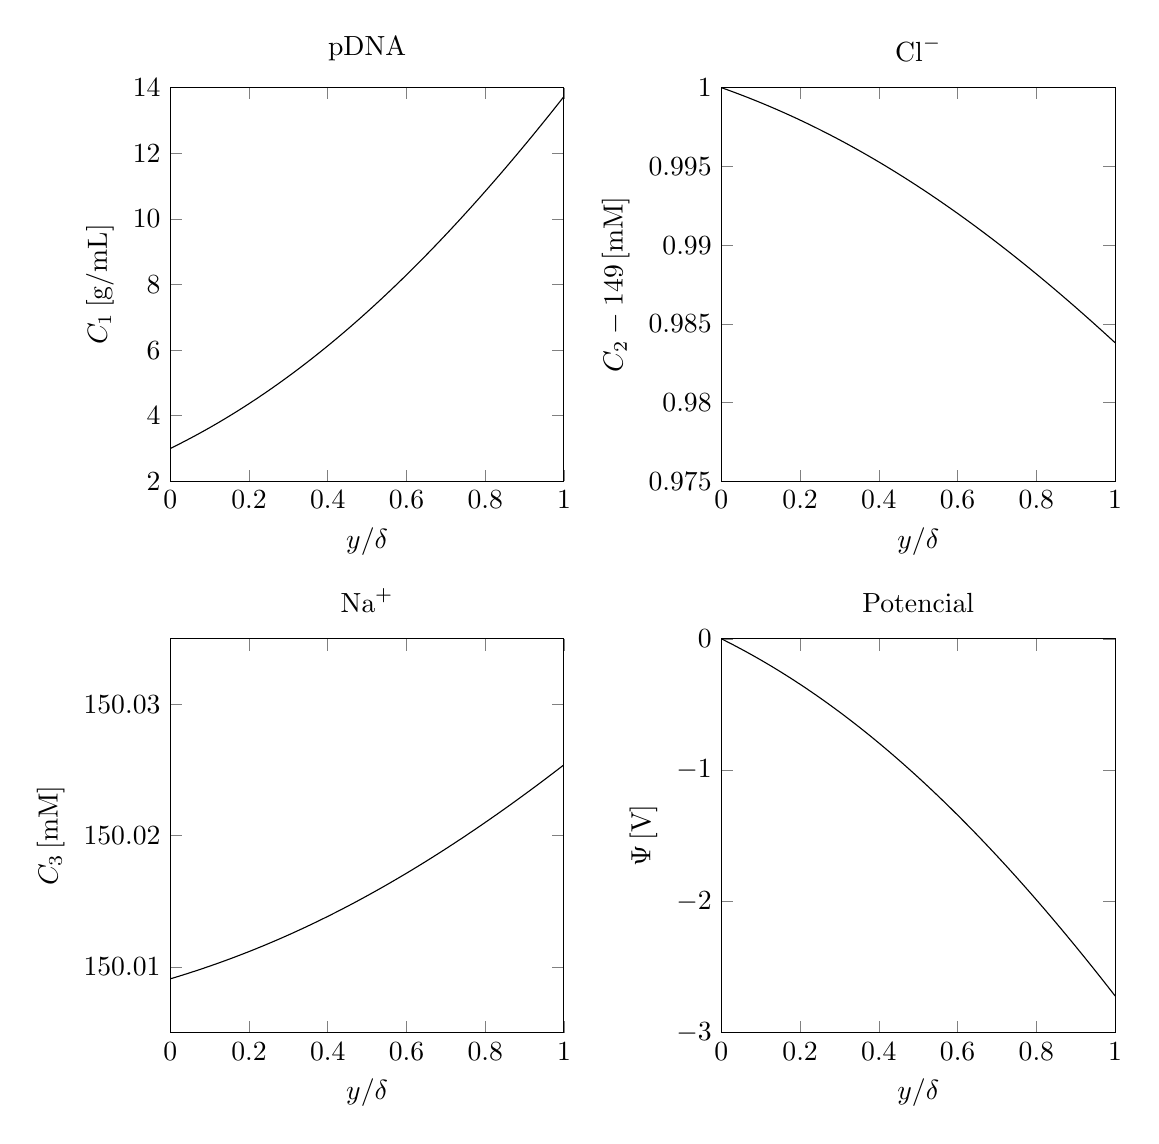
\begin{tikzpicture}
%\draw[help lines] (-2,-2)grid(13,13);
\begin{axis}[%
width=5cm,
height=5cm,
scale only axis,
xmin=0,
xmax=1,
xlabel={$y/\delta$},
ymin=2,
ymax=14,
ylabel={$C_1\,[\micro\mathrm{g}/\mathrm{mL}]$},
title={pDNA},
at={(0cm,7cm)},
anchor=south west
]
\addplot [
color=black,
solid,
forget plot
]
table[row sep=crcr]{
0 3\\
0.01 3.05931926752338\\
0.02 3.11955135344112\\
0.03 3.18070233365464\\
0.04 3.24277811802961\\
0.05 3.30578444695438\\
0.06 3.3697268880644\\
0.07 3.43461083313768\\
0.08 3.50044149516573\\
0.09 3.56722390560446\\
0.1 3.63496291180846\\
0.11 3.70366317465228\\
0.12 3.77332916634146\\
0.13 3.84396516841588\\
0.14 3.91557526994729\\
0.15 3.98816336593276\\
0.16 4.06173315588508\\
0.17 4.13628814262072\\
0.18 4.21183163124576\\
0.19 4.28836672833932\\
0.2 4.36589634133411\\
0.21 4.44442317809272\\
0.22 4.52394974667852\\
0.23 4.60447835531888\\
0.24 4.68601111255875\\
0.25 4.76854992760168\\
0.26 4.85209651083548\\
0.27 4.93665237453884\\
0.28 5.02221883376552\\
0.29 5.1087970074018\\
0.3 5.19638781939303\\
0.31 5.28499200013463\\
0.32 5.37461008802269\\
0.33 5.46524243115902\\
0.34 5.55688918920545\\
0.35 5.64955033538175\\
0.36 5.74322565860163\\
0.37 5.83791476574087\\
0.38 5.93361708403164\\
0.39 6.03033186357702\\
0.4 6.12805817997947\\
0.41 6.22679493707704\\
0.42 6.32654086978102\\
0.43 6.42729454700876\\
0.44 6.52905437470524\\
0.45 6.6318185989472\\
0.46 6.73558530912333\\
0.47 6.84035244118444\\
0.48 6.94611778095726\\
0.49 7.05287896751577\\
0.5 7.16063349660403\\
0.51 7.26937872410446\\
0.52 7.37911186954574\\
0.53 7.48983001964463\\
0.54 7.60153013187598\\
0.55 7.71420903806559\\
0.56 7.82786344800046\\
0.57 7.94248995305134\\
0.58 8.05808502980254\\
0.59 8.1746450436841\\
0.6 8.29216625260172\\
0.61 8.41064481055995\\
0.62 8.53007677127421\\
0.63 8.65045809176769\\
0.64 8.771784635949\\
0.65 8.89405217816694\\
0.66 9.01725640673872\\
0.67 9.14139292744836\\
0.68 9.2664572670119\\
0.69 9.3924448765066\\
0.7 9.5193511347612\\
0.71 9.64717135170451\\
0.72 9.7759007716701\\
0.73 9.90553457665455\\
0.74 10.0360678895273\\
0.75 10.1674957771901\\
0.76 10.2998132536844\\
0.77 10.4330152832446\\
0.78 10.5670967832967\\
0.79 10.7020526273996\\
0.8 10.8378776481294\\
0.81 10.9745666399046\\
0.82 11.1121143617518\\
0.83 11.2505155400108\\
0.84 11.3897648709795\\
0.85 11.5298570234963\\
0.86 11.6707866414615\\
0.87 11.8125483462961\\
0.88 11.9551367393388\\
0.89 12.09854640418\\
0.9 12.2427719089343\\
0.91 12.3878078084503\\
0.92 12.5336486464586\\
0.93 12.6802889576582\\
0.94 12.8277232697416\\
0.95 12.975946105359\\
0.96 13.1249519840222\\
0.97 13.274735423949\\
0.98 13.4252909438474\\
0.99 13.5766130646431\\
1 13.7286963111473\\
};
\end{axis}

\begin{axis}[%
width=5cm,
height=5cm,
scale only axis,
xmin=0,
xmax=1,
xlabel={$y/\delta$},
ymin=0.975,
ymax=1,
% scaled y ticks=manual:{$+149$}{%
% \pgfmathparse{#1-149}%
% },
yticklabel style={
/pgf/number format/fixed,
/pgf/number format/precision=3},
ylabel={$C_2-149\,[\mathrm{mM}]$},
% every axis y label/.style=
% {at={(ticklabel cs:0.5)},rotate=90,anchor=near ticklabel},
title={$\mathrm{Cl}^{-}$},
at={(7cm,7cm)},
anchor=south west
]
\addplot [
color=black,
solid,
forget plot
]
table[row sep=crcr]{
0 1\\
0.01 0.999910560665\\
0.02 0.999819739998\\
0.03 0.99972752882\\
0.04 0.999633918201\\
0.05 0.999538899471\\
0.06 0.999442464222\\
0.07 0.99934460431\\
0.08 0.999245311864\\
0.09 0.999144579288\\
0.1 0.999042399264\\
0.11 0.998938764759\\
0.12 0.998833669023\\
0.13 0.998727105597\\
0.14 0.998619068314\\
0.15 0.9985095513\\
0.16 0.998398548977\\
0.17 0.998286056067\\
0.18 0.99817206759\\
0.19 0.998056578867\\
0.2 0.997939585522\\
0.21 0.997821083481\\
0.22 0.997701068971\\
0.23 0.997579538525\\
0.24 0.997456488976\\
0.25 0.997331917461\\
0.26 0.997205821417\\
0.27 0.997078198582\\
0.28 0.996949046991\\
0.29 0.996818364979\\
0.3 0.996686151175\\
0.31 0.996552404501\\
0.32 0.996417124172\\
0.33 0.996280309687\\
0.34 0.996141960835\\
0.35 0.996002077686\\
0.36 0.995860660588\\
0.37 0.995717710166\\
0.38 0.995573227317\\
0.39 0.995427213206\\
0.4 0.995279669264\\
0.41 0.99513059718\\
0.42 0.9949799989\\
0.43 0.994827876621\\
0.44 0.994674232788\\
0.45 0.994519070086\\
0.46 0.994362391441\\
0.47 0.994204200007\\
0.48 0.994044499168\\
0.49 0.993883292531\\
0.5 0.993720583919\\
0.51 0.993556377365\\
0.52 0.993390677112\\
0.53 0.993223487602\\
0.54 0.993054813474\\
0.55 0.992884659555\\
0.56 0.992713030859\\
0.57 0.992539932579\\
0.58 0.992365370082\\
0.59 0.992189348901\\
0.6 0.992011874736\\
0.61 0.99183295344\\
0.62 0.991652591021\\
0.63 0.991470793632\\
0.64 0.991287567566\\
0.65 0.991102919255\\
0.66 0.990916855257\\
0.67 0.990729382257\\
0.68 0.990540507061\\
0.69 0.990350236587\\
0.7 0.990158577864\\
0.71 0.989965538025\\
0.72 0.9897711243\\
0.73 0.989575344017\\
0.74 0.989378204591\\
0.75 0.989179713523\\
0.76 0.988979878393\\
0.77 0.988778706856\\
0.78 0.988576206639\\
0.79 0.988372385534\\
0.8 0.988167251398\\
0.81 0.98796081214\\
0.82 0.987753075729\\
0.83 0.987544050178\\
0.84 0.987333743548\\
0.85 0.987122163942\\
0.86 0.986909319499\\
0.87 0.986695218392\\
0.88 0.986479868826\\
0.89 0.986263279032\\
0.9 0.986045457262\\
0.91 0.98582641179\\
0.92 0.985606150909\\
0.93 0.98538468292\\
0.94 0.98516201614\\
0.95 0.984938158889\\
0.96 0.984713119495\\
0.97 0.984486906286\\
0.98 0.98425952759\\
0.99 0.98403099173\\
1 0.983801307024\\
};
\end{axis}

\begin{axis}[%
width=5cm,
height=5cm,
scale only axis,
xmin=0,
xmax=1,
xlabel={$y/\delta$},
ymin=-3,
ymax=0,
ylabel={$\Psi\,[\micro\mathrm{V}]$},
title={Potencial},
at={(7cm,0cm)},
anchor=south west
]
\addplot [
color=black,
solid,
forget plot
]
table[row sep=crcr]{
0 0\\
0.01 -0.0150621458185117\\
0.02 -0.0303559992351976\\
0.03 -0.0458830922875105\\
0.04 -0.0616449145325243\\
0.05 -0.0776429121721861\\
0.06 -0.0938784872209881\\
0.07 -0.110352996717331\\
0.08 -0.12706775197975\\
0.09 -0.14402401790906\\
0.1 -0.161223012337395\\
0.11 -0.178665905424966\\
0.12 -0.196353819105302\\
0.13 -0.214287826579573\\
0.14 -0.232468951860529\\
0.15 -0.250898169366426\\
0.16 -0.269576403565246\\
0.17 -0.288504528669355\\
0.18 -0.307683368380665\\
0.19 -0.327113695686243\\
0.2 -0.346796232704181\\
0.21 -0.366731650579464\\
0.22 -0.386920569429453\\
0.23 -0.407363558338472\\
0.24 -0.428061135400937\\
0.25 -0.449013767812329\\
0.26 -0.470221872007226\\
0.27 -0.491685813843544\\
0.28 -0.513405908832019\\
0.29 -0.535382422409906\\
0.3 -0.557615570257787\\
0.31 -0.58010551865831\\
0.32 -0.602852384895616\\
0.33 -0.62585623769415\\
0.34 -0.649117097695505\\
0.35 -0.672634937971878\\
0.36 -0.696409684574704\\
0.37 -0.720441217116968\\
0.38 -0.744729369387663\\
0.39 -0.769273929996869\\
0.4 -0.794074643049844\\
0.41 -0.819131208848557\\
0.42 -0.844443284619057\\
0.43 -0.870010485263045\\
0.44 -0.895832384132049\\
0.45 -0.921908513822589\\
0.46 -0.948238366990692\\
0.47 -0.974821397184201\\
0.48 -1.00165701969124\\
0.49 -1.02874461240332\\
0.5 -1.05608351669146\\
0.51 -1.08367303829392\\
0.52 -1.11151244821389\\
0.53 -1.1396009836258\\
0.54 -1.16793784878878\\
0.55 -1.19652221596583\\
0.56 -1.22535322634737\\
0.57 -1.25442999097788\\
0.58 -1.28375159168428\\
0.59 -1.31331708200489\\
0.6 -1.3431254881177\\
0.61 -1.37317580976688\\
0.62 -1.40346702118634\\
0.63 -1.43399807201939\\
0.64 -1.46476788823342\\
0.65 -1.49577537302861\\
0.66 -1.52701940773991\\
0.67 -1.55849885273121\\
0.68 -1.59021254828108\\
0.69 -1.62215931545921\\
0.7 -1.65433795699282\\
0.71 -1.68674725812244\\
0.72 -1.71938598744636\\
0.73 -1.7522528977532\\
0.74 -1.78534672684206\\
0.75 -1.81866619832977\\
0.76 -1.85221002244472\\
0.77 -1.88597689680693\\
0.78 -1.919965507194\\
0.79 -1.95417452829254\\
0.8 -1.98860262443478\\
0.81 -2.02324845032025\\
0.82 -2.05811065172208\\
0.83 -2.09318786617792\\
0.84 -2.12847872366525\\
0.85 -2.16398184726092\\
0.86 -2.19969585378492\\
0.87 -2.2356193544282\\
0.88 -2.27175095536457\\
0.89 -2.30808925834672\\
0.9 -2.34463286128617\\
0.91 -2.38138035881748\\
0.92 -2.41833034284646\\
0.93 -2.45548140308271\\
0.94 -2.49283212755644\\
0.95 -2.53038110311975\\
0.96 -2.56812691593243\\
0.97 -2.60606815193256\\
0.98 -2.64420339729185\\
0.99 -2.68253123885618\\
1 -2.72105026457123\\
};
\end{axis}

\begin{axis}[%
	width=5cm,
	height=5cm,
	scale only axis,
	xmin=0,
	xmax=1,
	xlabel={$y/\delta$},
	ymin=150.005,
	ymax=150.035,
	ylabel={$C_3\,[\mathrm{mM}]$},
	every axis y label/.style=
	{at={(ticklabel cs:0.5)},rotate=90,anchor=near ticklabel},
	title={$\mathrm{Na}^{+}$},
	at={(0cm,0cm)},
	anchor=south west
	]
\addplot [
color=black,
solid,
forget plot
]
table[row sep=crcr]{
0 150.00909\\
0.01 150.009180298046\\
0.02 150.009271980599\\
0.03 150.00936505689\\
0.04 150.009459535898\\
0.05 150.009555426346\\
0.06 150.009652736693\\
0.07 150.009751475134\\
0.08 150.009851649594\\
0.09 150.009953267722\\
0.1 150.010056336887\\
0.11 150.010160864178\\
0.12 150.010266856397\\
0.13 150.010374320058\\
0.14 150.010483261382\\
0.15 150.010593686298\\
0.16 150.010705600439\\
0.17 150.010819009139\\
0.18 150.010933917432\\
0.19 150.011050330054\\
0.2 150.011168251436\\
0.21 150.01128768571\\
0.22 150.011408636703\\
0.23 150.011531107942\\
0.24 150.011655102647\\
0.25 150.011780623742\\
0.26 150.011907673845\\
0.27 150.012036255276\\
0.28 150.012166370057\\
0.29 150.012298019911\\
0.3 150.012431206268\\
0.31 150.012565930262\\
0.32 150.012702192738\\
0.33 150.012839994253\\
0.34 150.012979335078\\
0.35 150.013120215202\\
0.36 150.013262634333\\
0.37 150.013406591906\\
0.38 150.013552087081\\
0.39 150.013699118753\\
0.4 150.013847685549\\
0.41 150.013997785839\\
0.42 150.014149417735\\
0.43 150.014302579098\\
0.44 150.014457267543\\
0.45 150.014613480441\\
0.46 150.014771214927\\
0.47 150.014930467904\\
0.48 150.015091236045\\
0.49 150.015253515803\\
0.5 150.015417303413\\
0.51 150.015582594899\\
0.52 150.015749386077\\
0.53 150.015917672562\\
0.54 150.016087449773\\
0.55 150.01625871294\\
0.56 150.016431457106\\
0.57 150.016605677137\\
0.58 150.016781367722\\
0.59 150.016958523384\\
0.6 150.017137138481\\
0.61 150.017317207216\\
0.62 150.017498723638\\
0.63 150.01768168165\\
0.64 150.017866075013\\
0.65 150.018051897354\\
0.66 150.018239142169\\
0.67 150.018427802827\\
0.68 150.01861787258\\
0.69 150.018809344563\\
0.7 150.019002211803\\
0.71 150.01919646722\\
0.72 150.019392103638\\
0.73 150.019589113784\\
0.74 150.019787490296\\
0.75 150.019987225728\\
0.76 150.020188312551\\
0.77 150.020390743164\\
0.78 150.020594509892\\
0.79 150.020799604995\\
0.8 150.021006020671\\
0.81 150.021213749059\\
0.82 150.021422782245\\
0.83 150.021633112264\\
0.84 150.021844731107\\
0.85 150.022057630723\\
0.86 150.022271803023\\
0.87 150.022487239882\\
0.88 150.022703933147\\
0.89 150.022921874636\\
0.9 150.023141056146\\
0.91 150.02336146945\\
0.92 150.023583106307\\
0.93 150.023805958462\\
0.94 150.024030017647\\
0.95 150.024255275588\\
0.96 150.024481724007\\
0.97 150.024709354621\\
0.98 150.024938159149\\
0.99 150.025168129315\\
1 150.025399256846\\
};
\end{axis}
\end{tikzpicture}%
	\caption[Sistema de 3 componentes iónicos]{Perfis de concentração e potencial elétrico, obtidos por integração do sistema de equações diferenciais definido pela equação~\ref{eq:msmem}, para um sistema de 3 componentes iónicos (ver texto).}
	\label{fig:resexemploioes}
\end{figure}
\begin{figure}
	\centering
	%!TEX root=testfigum.tex
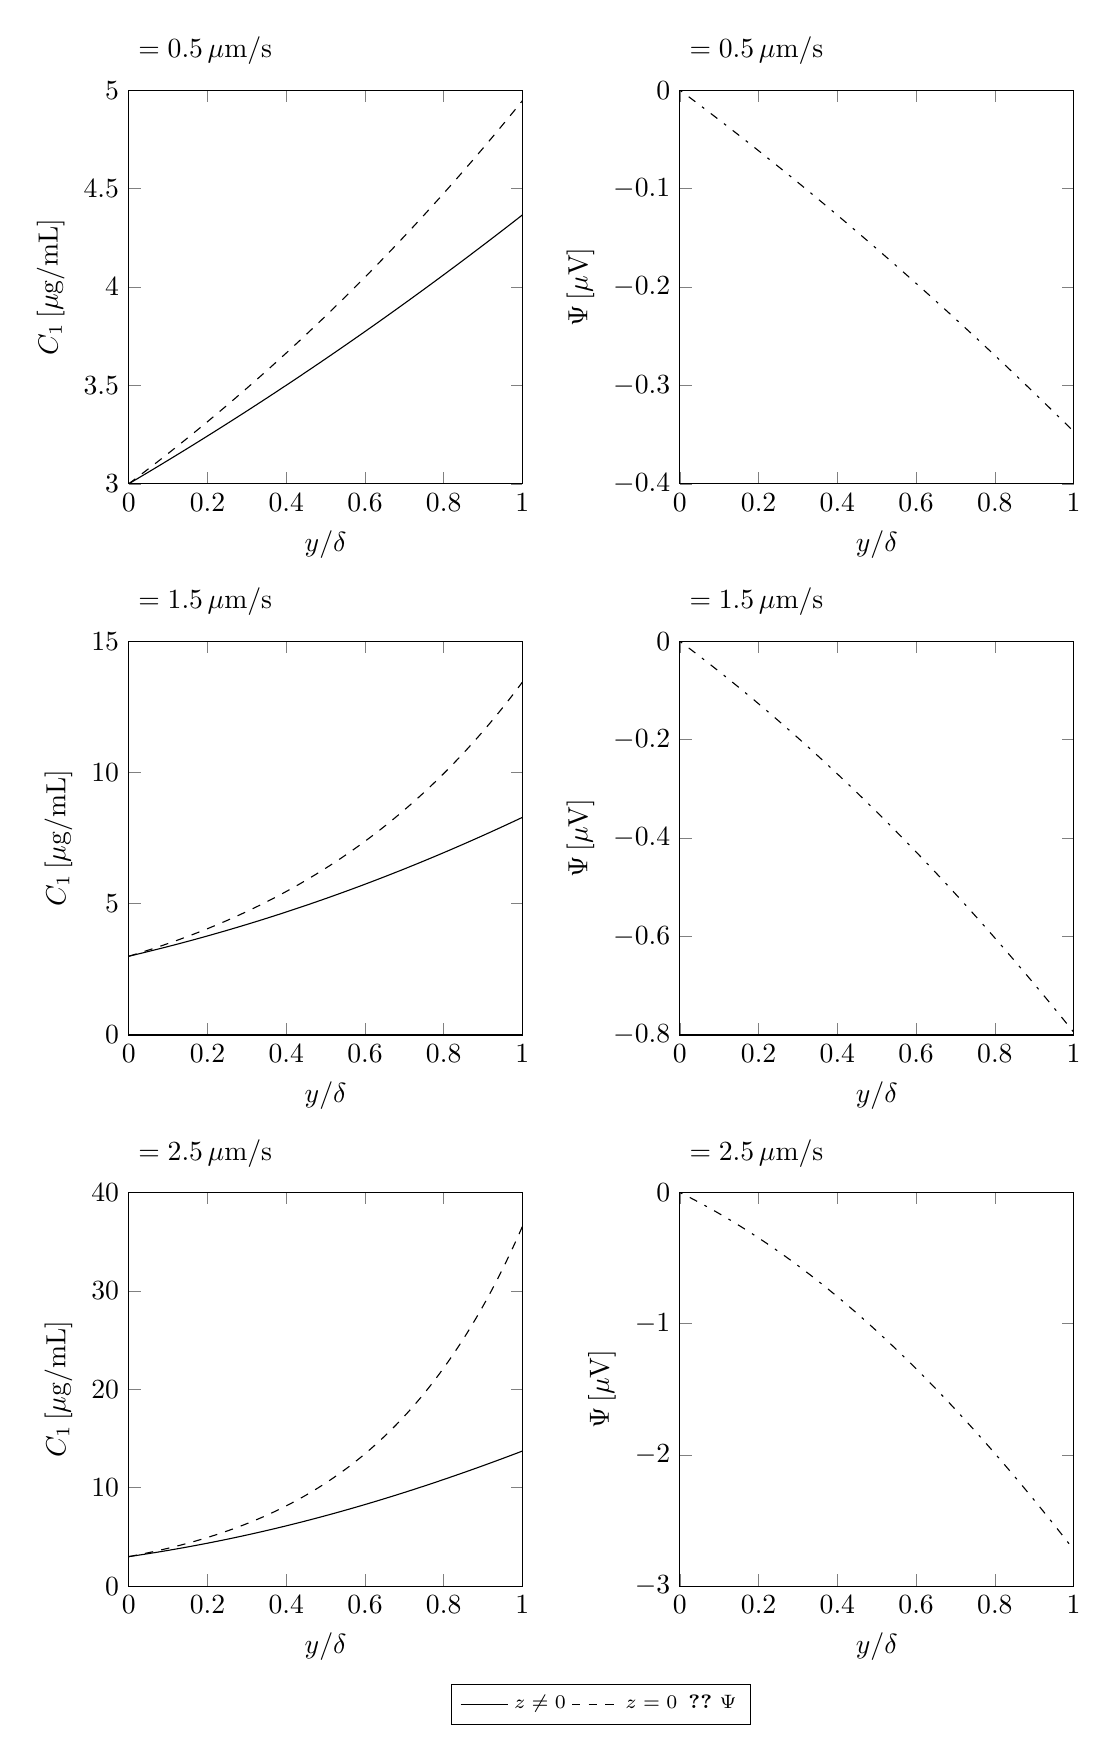
\begin{tikzpicture}

\node[right] at (0cm,19.5cm) {$\fluxo=0.5\,\mu$m/s};
\node[right] at (0cm,12.5cm) {$\fluxo=1.5\,\mu$m/s};
\node[right] at (0cm,5.5cm) {$\fluxo=2.5\,\mu$m/s};
\node[right] at (7cm,19.5cm) {$\fluxo=0.5\,\mu$m/s};
\node[right] at (7cm,12.5cm) {$\fluxo=1.5\,\mu$m/s};
\node[right] at (7cm,5.5cm) {$\fluxo=2.5\,\mu$m/s};
\begin{axis}[%
width=5cm,
height=5cm,
scale only axis,
xmin=0,
xmax=1,
ymin=0,
ymax=15,
xlabel={$y/\delta$},
ylabel={$C_1$\,[$\mu$g/mL]},
at={(0cm,7cm)},
anchor=south west,
]
\addplot [
color=black,
solid,
forget plot
]
table[row sep=crcr]{
0 3\\
0.01 3.0354823680814\\
0.02 3.07129246249783\\
0.03 3.10743161685481\\
0.04 3.14390114360928\\
0.05 3.1807023337895\\
0.06 3.21783645672229\\
0.07 3.2553047597679\\
0.08 3.29310846806266\\
0.09 3.33124878426948\\
0.1 3.36972688833641\\
0.11 3.40854393726328\\
0.12 3.44770106487676\\
0.13 3.48719938161364\\
0.14 3.52703997431273\\
0.15 3.5672239060153\\
0.16 3.60775221577427\\
0.17 3.64862591847212\\
0.18 3.68984600464767\\
0.19 3.73141344033181\\
0.2 3.77332916689225\\
0.21 3.81559410088725\\
0.22 3.85820913392847\\
0.23 3.90117513255304\\
0.24 3.94449293810467\\
0.25 3.98816336662408\\
0.26 4.03218720874859\\
0.27 4.07656522962093\\
0.28 4.12129816880732\\
0.29 4.16638674022479\\
0.3 4.21183163207765\\
0.31 4.25763350680323\\
0.32 4.30379300102678\\
0.33 4.35031072552548\\
0.34 4.39718726520162\\
0.35 4.44442317906477\\
0.36 4.49201900022295\\
0.37 4.53997523588285\\
0.38 4.5882923673588\\
0.39 4.63697085009058\\
0.4 4.68601111367005\\
0.41 4.73541356187626\\
0.42 4.78517857271924\\
0.43 4.83530649849218\\
0.44 4.885797665832\\
0.45 4.93665237578812\\
0.46 4.98787090389938\\
0.47 5.03945350027897\\
0.48 5.09140038970728\\
0.49 5.14371177173246\\
0.5 5.19638782077863\\
0.51 5.24942868626161\\
0.52 5.30283449271195\\
0.53 5.35660533990523\\
0.54 5.4107413029994\\
0.55 5.46524243267898\\
0.56 5.52010875530612\\
0.57 5.57534027307814\\
0.58 5.63093696419165\\
0.59 5.68689878301278\\
0.6 5.7432256602537\\
0.61 5.79991750315492\\
0.62 5.8569741956735\\
0.63 5.91439559867678\\
0.64 5.97218155014159\\
0.65 6.03033186535871\\
0.66 6.08884633714239\\
0.67 6.14772473604479\\
0.68 6.20696681057521\\
0.69 6.2665722874238\\
0.7 6.32654087168968\\
0.71 6.38687224711325\\
0.72 6.44756607631258\\
0.73 6.50862200102357\\
0.74 6.57003964234381\\
0.75 6.63181860097999\\
0.76 6.6939584574985\\
0.77 6.75645877257934\\
0.78 6.81931908727284\\
0.79 6.88253892325932\\
0.8 6.94611778311124\\
0.81 7.01005515055793\\
0.82 7.07435049075252\\
0.83 7.13900325054106\\
0.84 7.2040128587335\\
0.85 7.2693787263766\\
0.86 7.33510024702833\\
0.87 7.40117679703388\\
0.88 7.46760773580283\\
0.89 7.53439240608768\\
0.9 7.60153013426318\\
0.91 7.66902023060671\\
0.92 7.73686198957923\\
0.93 7.80505469010688\\
0.94 7.87359759586302\\
0.95 7.9424899555505\\
0.96 8.01173100318412\\
0.97 8.08131995837313\\
0.98 8.1512560266036\\
0.99 8.22153839952054\\
1 8.2921662552097\\
};

\addplot [
color=black,
dashed,
forget plot
]
table[row sep=crcr]{
0 3\\
0.01 3.04533919384716\\
0.02 3.09136360186055\\
0.03 3.13808357972615\\
0.04 3.18550963963608\\
0.05 3.23365245265389\\
0.06 3.28252285111563\\
0.07 3.33213183106712\\
0.08 3.38249055473813\\
0.09 3.43361035305394\\
0.1 3.48550272818485\\
0.11 3.53817935613417\\
0.12 3.59165208936543\\
0.13 3.64593295946919\\
0.14 3.70103417987023\\
0.15 3.75696814857559\\
0.16 3.81374745096421\\
0.17 3.87138486261867\\
0.18 3.92989335219974\\
0.19 3.98928608436442\\
0.2 4.04957642272801\\
0.21 4.11077793287099\\
0.22 4.17290438539134\\
0.23 4.23596975900298\\
0.24 4.29998824368102\\
0.25 4.3649742438546\\
0.26 4.43094238164793\\
0.27 4.4979075001703\\
0.28 4.5658846668559\\
0.29 4.63488917685402\\
0.3 4.70493655647051\\
0.31 4.7760425666613\\
0.32 4.84822320657868\\
0.33 4.92149471717113\\
0.34 4.99587358483766\\
0.35 5.07137654513727\\
0.36 5.14802058655458\\
0.37 5.22582295432222\\
0.38 5.30480115430121\\
0.39 5.3849729569197\\
0.4 5.46635640117153\\
0.41 5.54896979867498\\
0.42 5.63283173779303\\
0.43 5.71796108781577\\
0.44 5.80437700320609\\
0.45 5.89209892790954\\
0.46 5.98114659972925\\
0.47 6.07154005476704\\
0.48 6.16329963193166\\
0.49 6.25644597751508\\
0.5 6.35100004983802\\
0.51 6.44698312396566\\
0.52 6.5444167964946\\
0.53 6.64332299041222\\
0.54 6.74372396002941\\
0.55 6.84564229598791\\
0.56 6.94910093034328\\
0.57 7.05412314172471\\
0.58 7.16073256057283\\
0.59 7.26895317445665\\
0.6 7.37880933347085\\
0.61 7.49032575571467\\
0.62 7.60352753285356\\
0.63 7.71844013576498\\
0.64 7.83508942026935\\
0.65 7.95350163294782\\
0.66 8.07370341704779\\
0.67 8.19572181847778\\
0.68 8.31958429189289\\
0.69 8.44531870687219\\
0.7 8.57295335418949\\
0.71 8.7025169521789\\
0.72 8.83403865319657\\
0.73 8.96754805018009\\
0.74 9.10307518330703\\
0.75 9.24065054675409\\
0.76 9.38030509555847\\
0.77 9.5220702525828\\
0.78 9.6659779155855\\
0.79 9.81206046439785\\
0.8 9.96035076820964\\
0.81 10.1108821929648\\
0.82 10.263688608869\\
0.83 10.4188043980105\\
0.84 10.5762644620961\\
0.85 10.7361042303047\\
0.86 10.8983596672584\\
0.87 11.0630672811151\\
0.88 11.2302641317826\\
0.89 11.3999878392578\\
0.9 11.5722765920909\\
0.91 11.7471691559782\\
0.92 11.9247048824842\\
0.93 12.1049237178966\\
0.94 12.2878662122135\\
0.95 12.473573528268\\
0.96 12.6620874509897\\
0.97 12.8534503968064\\
0.98 13.0477054231882\\
0.99 13.2448962383357\\
1 13.4450672110142\\
};
\end{axis}

\begin{axis}[%
width=5cm,
height=5cm,
scale only axis,
xmin=0,
xmax=1,
ymin=3,
ymax=5,
xlabel={$y/\delta$},
ylabel={$C_1$\,[$\mu$g/mL]},
at={(0cm,14cm)},
anchor=south west,
]
\addplot [
color=black,
solid,
forget plot
]
table[row sep=crcr]{
0 3\\
0.01 3.01179112517423\\
0.02 3.02361856448047\\
0.03 3.03548236808536\\
0.04 3.04738258589917\\
0.05 3.05931926757465\\
0.06 3.07129246250577\\
0.07 3.08330221982657\\
0.08 3.09534858841001\\
0.09 3.10743161686673\\
0.1 3.11955135354401\\
0.11 3.13170784652451\\
0.12 3.14390114362521\\
0.13 3.15613129239629\\
0.14 3.16839834011998\\
0.15 3.18070233380946\\
0.16 3.1930433202078\\
0.17 3.20542134578688\\
0.18 3.21783645674627\\
0.19 3.23028869901224\\
0.2 3.24277811823664\\
0.21 3.25530475979593\\
0.22 3.2678686687901\\
0.23 3.28046989004168\\
0.24 3.29310846809475\\
0.25 3.30578444721389\\
0.26 3.31849787138328\\
0.27 3.33124878430564\\
0.28 3.34403722940134\\
0.29 3.35686324980742\\
0.3 3.36972688837664\\
0.31 3.3826281876766\\
0.32 3.39556718998877\\
0.33 3.40854393730761\\
0.34 3.42155847133971\\
0.35 3.43461083350285\\
0.36 3.44770106492519\\
0.37 3.46082920644436\\
0.38 3.47399529860665\\
0.39 3.48719938166617\\
0.4 3.50044149558404\\
0.41 3.51372168002755\\
0.42 3.52703997436937\\
0.43 3.54039641768681\\
0.44 3.55379104876098\\
0.45 3.56722390607607\\
0.46 3.58069502781859\\
0.47 3.59420445187664\\
0.48 3.60775221583917\\
0.49 3.62133835699528\\
0.5 3.63496291233351\\
0.51 3.64862591854115\\
0.52 3.6623274120036\\
0.53 3.67606742880364\\
0.54 3.68984600472084\\
0.55 3.70366317523088\\
0.56 3.71751897550495\\
0.57 3.73141344040913\\
0.58 3.74534660450376\\
0.59 3.7593185020429\\
0.6 3.77332916697372\\
0.61 3.78737863293593\\
0.62 3.80146693326125\\
0.63 3.81559410097286\\
0.64 3.82976016878489\\
0.65 3.84396516910186\\
0.66 3.85820913401824\\
0.67 3.87249209531791\\
0.68 3.8868140844737\\
0.69 3.90117513264696\\
0.7 3.91557527068705\\
0.71 3.93001452913093\\
0.72 3.94449293820275\\
0.73 3.95901052781342\\
0.74 3.9735673275602\\
0.75 3.98816336672632\\
0.76 4.00279867428063\\
0.77 4.0174732788772\\
0.78 4.03218720885499\\
0.79 4.04694049223749\\
0.8 4.06173315673244\\
0.81 4.07656522973148\\
0.82 4.09143673830987\\
0.83 4.10634770922618\\
0.84 4.12129816892204\\
0.85 4.13628814352188\\
0.86 4.15131765883266\\
0.87 4.16638674034366\\
0.88 4.18149541322623\\
0.89 4.1966437023336\\
0.9 4.21183163220067\\
0.91 4.22705922704383\\
0.92 4.24232651076079\\
0.93 4.2576335069304\\
0.94 4.27298023881254\\
0.95 4.28836672934794\\
0.96 4.3037930011581\\
0.97 4.31925907654513\\
0.98 4.33476497749171\\
0.99 4.35031072566095\\
1 4.36589634239635\\
};
\addplot [
color=black,
dashed,
forget plot
]
table[row sep=crcr]{
0 3\\
0.01 3.0150375625782\\
0.02 3.0301505012525\\
0.03 3.04533919384716\\
0.04 3.06060402008027\\
0.05 3.07594536157329\\
0.06 3.09136360186055\\
0.07 3.10685912639887\\
0.08 3.12243232257716\\
0.09 3.13808357972615\\
0.1 3.15381328912807\\
0.11 3.16962184402648\\
0.12 3.18550963963608\\
0.13 3.20147707315258\\
0.14 3.21752454376265\\
0.15 3.23365245265389\\
0.16 3.24986120302488\\
0.17 3.2661512000952\\
0.18 3.28252285111563\\
0.19 3.29897656537831\\
0.2 3.31551275422694\\
0.21 3.33213183106712\\
0.22 3.34883421137661\\
0.23 3.36562031271581\\
0.24 3.38249055473813\\
0.25 3.39944535920048\\
0.26 3.41648514997387\\
0.27 3.43361035305394\\
0.28 3.45082139657168\\
0.29 3.46811871080406\\
0.3 3.48550272818485\\
0.31 3.50297388331538\\
0.32 3.52053261297543\\
0.33 3.53817935613417\\
0.34 3.5559145539611\\
0.35 3.57373864983707\\
0.36 3.59165208936543\\
0.37 3.60965532038309\\
0.38 3.62774879297175\\
0.39 3.64593295946919\\
0.4 3.66420827448051\\
0.41 3.68257519488953\\
0.42 3.70103417987023\\
0.43 3.71958569089818\\
0.44 3.73823019176214\\
0.45 3.75696814857559\\
0.46 3.77580002978843\\
0.47 3.79472630619868\\
0.48 3.81374745096421\\
0.49 3.83286393961466\\
0.5 3.85207625006322\\
0.51 3.87138486261867\\
0.52 3.89079025999732\\
0.53 3.91029292733511\\
0.54 3.92989335219974\\
0.55 3.94959202460286\\
0.56 3.96938943701231\\
0.57 3.98928608436442\\
0.58 4.00928246407642\\
0.59 4.02937907605883\\
0.6 4.04957642272801\\
0.61 4.06987500901867\\
0.62 4.09027534239653\\
0.63 4.11077793287099\\
0.64 4.13138329300787\\
0.65 4.15209193794225\\
0.66 4.17290438539134\\
0.67 4.1938211556674\\
0.68 4.21484277169078\\
0.69 4.23596975900298\\
0.7 4.25720264577977\\
0.71 4.27854196284444\\
0.72 4.29998824368102\\
0.73 4.32154202444765\\
0.74 4.34320384398997\\
0.75 4.3649742438546\\
0.76 4.38685376830267\\
0.77 4.40884296432343\\
0.78 4.43094238164793\\
0.79 4.45315257276274\\
0.8 4.47547409292381\\
0.81 4.4979075001703\\
0.82 4.52045335533856\\
0.83 4.54311222207614\\
0.84 4.5658846668559\\
0.85 4.58877125899014\\
0.86 4.61177257064484\\
0.87 4.63488917685402\\
0.88 4.65812165553401\\
0.89 4.681470587498\\
0.9 4.70493655647051\\
0.91 4.72852014910197\\
0.92 4.75222195498345\\
0.93 4.7760425666613\\
0.94 4.79998257965208\\
0.95 4.82404259245735\\
0.96 4.84822320657868\\
0.97 4.87252502653269\\
0.98 4.89694865986614\\
0.99 4.92149471717113\\
1 4.94616381210038\\
};
\end{axis}

\begin{axis}[%
width=5cm,
height=5cm,
scale only axis,
xmin=0,
xmax=1,
ymin=-0.4,
ymax=0,
xlabel={$y/\delta$},
ylabel={$\Psi$\,[$\mu$V]},
at={(7cm,14cm)},
anchor=south west,
]
\addplot [
color=black,
dash pattern=on 1pt off 3pt on 3pt off 3pt,
forget plot
]
table[row sep=crcr]{
0 0\\
0.01 -0.00299396750040809\\
0.02 -0.00599715321126341\\
0.03 -0.00900956978790304\\
0.04 -0.0120312298200606\\
0.05 -0.0150621458315603\\
0.06 -0.0181023302800137\\
0.07 -0.0211517955565191\\
0.08 -0.0242105539853628\\
0.09 -0.0272786178237238\\
0.1 -0.0303559992613806\\
0.11 -0.0334427104204201\\
0.12 -0.0365387633549506\\
0.13 -0.0396441700508155\\
0.14 -0.0427589424253115\\
0.15 -0.0458830923269078\\
0.16 -0.0490166315349694\\
0.17 -0.0521595717594821\\
0.18 -0.055311924640781\\
0.19 -0.0584737017492807\\
0.2 -0.0616449145852094\\
0.21 -0.0648255745783449\\
0.22 -0.0680156930877542\\
0.23 -0.0712152814015349\\
0.24 -0.07442435073656\\
0.25 -0.0776429122382259\\
0.26 -0.0808709769802023\\
0.27 -0.0841085559641856\\
0.28 -0.0873556601196553\\
0.29 -0.0906123003036328\\
0.3 -0.0938784873004431\\
0.31 -0.0971542318214803\\
0.32 -0.100439544504975\\
0.33 -0.103734435915763\\
0.34 -0.107038916545065\\
0.35 -0.110352996810256\\
0.36 -0.113676687054648\\
0.37 -0.117009997547273\\
0.38 -0.120352938482671\\
0.39 -0.123705519980671\\
0.4 -0.127067752086192\\
0.41 -0.13043964476903\\
0.42 -0.13382120792366\\
0.43 -0.137212451369036\\
0.44 -0.140613384848395\\
0.45 -0.144024018029062\\
0.46 -0.147444360502261\\
0.47 -0.150874421782932\\
0.48 -0.154314211309539\\
0.49 -0.157763738443897\\
0.5 -0.161223012470991\\
0.51 -0.164692042598803\\
0.52 -0.168170837958136\\
0.53 -0.171659407602454\\
0.54 -0.17515776050771\\
0.55 -0.178665905572188\\
0.56 -0.182183851616341\\
0.57 -0.185711607382641\\
0.58 -0.18924918153542\\
0.59 -0.192796582660725\\
0.6 -0.196353819266172\\
0.61 -0.199920899780801\\
0.62 -0.203497832554939\\
0.63 -0.20708462586006\\
0.64 -0.210681287888658\\
0.65 -0.21428782675411\\
0.66 -0.217904250490553\\
0.67 -0.221530567052761\\
0.68 -0.225166784316023\\
0.69 -0.228812910076027\\
0.7 -0.232468952048744\\
0.71 -0.236134917870321\\
0.72 -0.239810815096972\\
0.73 -0.243496651204871\\
0.74 -0.247192433590055\\
0.75 -0.250898169568326\\
0.76 -0.254613866375153\\
0.77 -0.258339531165584\\
0.78 -0.262075171014158\\
0.79 -0.265820792914818\\
0.8 -0.269576403780832\\
0.81 -0.273342010444711\\
0.82 -0.27711761965814\\
0.83 -0.2809032380919\\
0.84 -0.284698872335801\\
0.85 -0.288504528898621\\
0.86 -0.292320214208038\\
0.87 -0.296145934610572\\
0.88 -0.299981696371534\\
0.89 -0.303827505674968\\
0.9 -0.307683368623603\\
0.91 -0.311549291238811\\
0.92 -0.315425279460557\\
0.93 -0.319311339147366\\
0.94 -0.323207476076282\\
0.95 -0.327113695942838\\
0.96 -0.331030004361022\\
0.97 -0.334956406863253\\
0.98 -0.33889290890036\\
0.99 -0.342839515841552\\
1 -0.346796232974411\\
};\label{pgf:pot};
\end{axis}

\begin{axis}[%
width=5cm,
height=5cm,
scale only axis,
xmin=0,
xmax=1,
ymin=-0.8,
ymax=0,
xlabel={$y/\delta$},
ylabel={$\Psi$\,[$\mu$V]},
at={(7cm,7cm)},
anchor=south west,
]
\addplot [
color=black,
dash pattern=on 1pt off 3pt on 3pt off 3pt,
forget plot
]
table[row sep=crcr]{
0 0\\
0.01 -0.00599715321113721\\
0.02 -0.0120312298198078\\
0.03 -0.0181023302796341\\
0.04 -0.0242105539848561\\
0.05 -0.0303559992607464\\
0.06 -0.0365387633541886\\
0.07 -0.0427589424244214\\
0.08 -0.0490166315339509\\
0.09 -0.0553119246396339\\
0.1 -0.0616449145839333\\
0.11 -0.0680156930863491\\
0.12 -0.0744243507350254\\
0.13 -0.0808709769785379\\
0.14 -0.0873556601178611\\
0.15 -0.093878487298519\\
0.16 -0.10043954450292\\
0.17 -0.10703891654288\\
0.18 -0.113676687052332\\
0.19 -0.120352938480225\\
0.2 -0.127067752083615\\
0.21 -0.133821207920952\\
0.22 -0.140613384845556\\
0.23 -0.14744436049929\\
0.24 -0.154314211306436\\
0.25 -0.161223012467757\\
0.26 -0.16817083795477\\
0.27 -0.175157760504212\\
0.28 -0.182183851612711\\
0.29 -0.189249181531658\\
0.3 -0.196353819262277\\
0.31 -0.203497832550912\\
0.32 -0.210681287884499\\
0.33 -0.217904250486261\\
0.34 -0.225166784311599\\
0.35 -0.232468952044187\\
0.36 -0.239810815092283\\
0.37 -0.247192433585234\\
0.38 -0.254613866370199\\
0.39 -0.262075171009072\\
0.4 -0.269576403775613\\
0.41 -0.277117619652789\\
0.42 -0.284698872330318\\
0.43 -0.292320214202422\\
0.44 -0.299981696365786\\
0.45 -0.307683368617723\\
0.46 -0.315425279454545\\
0.47 -0.323207476070137\\
0.48 -0.331030004354745\\
0.49 -0.338892908893951\\
0.5 -0.34679623296787\\
0.51 -0.354740018550542\\
0.52 -0.362724306309518\\
0.53 -0.370749135605667\\
0.54 -0.378814544493162\\
0.55 -0.386920569719678\\
0.56 -0.39506724672679\\
0.57 -0.403254609650557\\
0.58 -0.411482691322311\\
0.59 -0.419751523269641\\
0.6 -0.428061135717565\\
0.61 -0.436411557589899\\
0.62 -0.444802816510814\\
0.63 -0.453234938806584\\
0.64 -0.461707949507519\\
0.65 -0.47022187235009\\
0.66 -0.478776729779232\\
0.67 -0.487372542950835\\
0.68 -0.49600933173441\\
0.69 -0.504687114715943\\
0.7 -0.513405909200921\\
0.71 -0.52216573121753\\
0.72 -0.530966595520037\\
0.73 -0.539808515592337\\
0.74 -0.548691503651668\\
0.75 -0.557615570652499\\
0.76 -0.566580726290583\\
0.77 -0.575586979007168\\
0.78 -0.584634335993376\\
0.79 -0.593722803194738\\
0.8 -0.602852385315885\\
0.81 -0.612023085825399\\
0.82 -0.621234906960806\\
0.83 -0.630487849733732\\
0.84 -0.639781913935196\\
0.85 -0.649117098141054\\
0.86 -0.658493399717584\\
0.87 -0.667910814827211\\
0.88 -0.677369338434373\\
0.89 -0.686868964311517\\
0.9 -0.696409685045235\\
0.91 -0.705991492042522\\
0.92 -0.715614375537172\\
0.93 -0.725278324596288\\
0.94 -0.734983327126928\\
0.95 -0.744729369882857\\
0.96 -0.754516438471427\\
0.97 -0.76434451736057\\
0.98 -0.774213589885898\\
0.99 -0.784123638257922\\
1 -0.794074643569366\\
};
\end{axis}

\begin{axis}[%
width=5cm,
height=5cm,
scale only axis,
xmin=0,
xmax=1,
ymin=-3,
ymax=0,
xlabel={$y/\delta$},
ylabel={$\Psi$\,[$\mu$V]},
at={(7cm,0cm)},
anchor=south west,
]
\addplot [
color=black,
dash pattern=on 1pt off 3pt on 3pt off 3pt,
forget plot,
]
table[row sep=crcr]{
0 0\\
0.01 -0.0150621458185117\\
0.02 -0.0303559992351976\\
0.03 -0.0458830922875105\\
0.04 -0.0616449145325243\\
0.05 -0.0776429121721861\\
0.06 -0.0938784872209881\\
0.07 -0.110352996717331\\
0.08 -0.12706775197975\\
0.09 -0.14402401790906\\
0.1 -0.161223012337395\\
0.11 -0.178665905424966\\
0.12 -0.196353819105302\\
0.13 -0.214287826579573\\
0.14 -0.232468951860529\\
0.15 -0.250898169366426\\
0.16 -0.269576403565246\\
0.17 -0.288504528669355\\
0.18 -0.307683368380665\\
0.19 -0.327113695686243\\
0.2 -0.346796232704181\\
0.21 -0.366731650579464\\
0.22 -0.386920569429453\\
0.23 -0.407363558338472\\
0.24 -0.428061135400937\\
0.25 -0.449013767812329\\
0.26 -0.470221872007226\\
0.27 -0.491685813843544\\
0.28 -0.513405908832019\\
0.29 -0.535382422409906\\
0.3 -0.557615570257787\\
0.31 -0.58010551865831\\
0.32 -0.602852384895616\\
0.33 -0.62585623769415\\
0.34 -0.649117097695505\\
0.35 -0.672634937971878\\
0.36 -0.696409684574704\\
0.37 -0.720441217116968\\
0.38 -0.744729369387663\\
0.39 -0.769273929996869\\
0.4 -0.794074643049844\\
0.41 -0.819131208848557\\
0.42 -0.844443284619057\\
0.43 -0.870010485263045\\
0.44 -0.895832384132049\\
0.45 -0.921908513822589\\
0.46 -0.948238366990692\\
0.47 -0.974821397184201\\
0.48 -1.00165701969124\\
0.49 -1.02874461240332\\
0.5 -1.05608351669146\\
0.51 -1.08367303829392\\
0.52 -1.11151244821389\\
0.53 -1.1396009836258\\
0.54 -1.16793784878878\\
0.55 -1.19652221596583\\
0.56 -1.22535322634737\\
0.57 -1.25442999097788\\
0.58 -1.28375159168428\\
0.59 -1.31331708200489\\
0.6 -1.3431254881177\\
0.61 -1.37317580976688\\
0.62 -1.40346702118634\\
0.63 -1.43399807201939\\
0.64 -1.46476788823342\\
0.65 -1.49577537302861\\
0.66 -1.52701940773991\\
0.67 -1.55849885273121\\
0.68 -1.59021254828108\\
0.69 -1.62215931545921\\
0.7 -1.65433795699282\\
0.71 -1.68674725812244\\
0.72 -1.71938598744636\\
0.73 -1.7522528977532\\
0.74 -1.78534672684206\\
0.75 -1.81866619832977\\
0.76 -1.85221002244472\\
0.77 -1.88597689680693\\
0.78 -1.919965507194\\
0.79 -1.95417452829254\\
0.8 -1.98860262443478\\
0.81 -2.02324845032025\\
0.82 -2.05811065172208\\
0.83 -2.09318786617792\\
0.84 -2.12847872366525\\
0.85 -2.16398184726092\\
0.86 -2.19969585378492\\
0.87 -2.2356193544282\\
0.88 -2.27175095536457\\
0.89 -2.30808925834672\\
0.9 -2.34463286128617\\
0.91 -2.38138035881748\\
0.92 -2.41833034284646\\
0.93 -2.45548140308271\\
0.94 -2.49283212755644\\
0.95 -2.53038110311975\\
0.96 -2.56812691593243\\
0.97 -2.60606815193256\\
0.98 -2.64420339729185\\
0.99 -2.68253123885618\\
1 -2.72105026457123\\
};
\end{axis}

\begin{axis}[%
width=5cm,
height=5cm,
scale only axis,
xmin=0,
xmax=1,
ymin=0,
ymax=40,
xlabel={$y/\delta$},
ylabel={$C_1$\,[$\mu$g/mL]},
at={(0cm,0cm)},
anchor=south west,
legend style={at={(6cm,-1.5cm)},legend columns=-1,anchor=center,font=\scriptsize,draw=black,fill=white,legend cell align=left}
]
\addplot [
color=black,
solid,
]
table[row sep=crcr]{
0 3\\
0.01 3.05931926752338\\
0.02 3.11955135344112\\
0.03 3.18070233365464\\
0.04 3.24277811802961\\
0.05 3.30578444695438\\
0.06 3.3697268880644\\
0.07 3.43461083313768\\
0.08 3.50044149516573\\
0.09 3.56722390560446\\
0.1 3.63496291180846\\
0.11 3.70366317465228\\
0.12 3.77332916634146\\
0.13 3.84396516841588\\
0.14 3.91557526994729\\
0.15 3.98816336593276\\
0.16 4.06173315588508\\
0.17 4.13628814262072\\
0.18 4.21183163124576\\
0.19 4.28836672833932\\
0.2 4.36589634133411\\
0.21 4.44442317809272\\
0.22 4.52394974667852\\
0.23 4.60447835531888\\
0.24 4.68601111255875\\
0.25 4.76854992760168\\
0.26 4.85209651083548\\
0.27 4.93665237453884\\
0.28 5.02221883376552\\
0.29 5.1087970074018\\
0.3 5.19638781939303\\
0.31 5.28499200013463\\
0.32 5.37461008802269\\
0.33 5.46524243115902\\
0.34 5.55688918920545\\
0.35 5.64955033538175\\
0.36 5.74322565860163\\
0.37 5.83791476574087\\
0.38 5.93361708403164\\
0.39 6.03033186357702\\
0.4 6.12805817997947\\
0.41 6.22679493707704\\
0.42 6.32654086978102\\
0.43 6.42729454700876\\
0.44 6.52905437470524\\
0.45 6.6318185989472\\
0.46 6.73558530912333\\
0.47 6.84035244118444\\
0.48 6.94611778095726\\
0.49 7.05287896751577\\
0.5 7.16063349660403\\
0.51 7.26937872410446\\
0.52 7.37911186954574\\
0.53 7.48983001964463\\
0.54 7.60153013187598\\
0.55 7.71420903806559\\
0.56 7.82786344800046\\
0.57 7.94248995305134\\
0.58 8.05808502980254\\
0.59 8.1746450436841\\
0.6 8.29216625260172\\
0.61 8.41064481055995\\
0.62 8.53007677127421\\
0.63 8.65045809176769\\
0.64 8.771784635949\\
0.65 8.89405217816694\\
0.66 9.01725640673872\\
0.67 9.14139292744836\\
0.68 9.2664572670119\\
0.69 9.3924448765066\\
0.7 9.5193511347612\\
0.71 9.64717135170451\\
0.72 9.7759007716701\\
0.73 9.90553457665455\\
0.74 10.0360678895273\\
0.75 10.1674957771901\\
0.76 10.2998132536844\\
0.77 10.4330152832446\\
0.78 10.5670967832967\\
0.79 10.7020526273996\\
0.8 10.8378776481294\\
0.81 10.9745666399046\\
0.82 11.1121143617518\\
0.83 11.2505155400108\\
0.84 11.3897648709795\\
0.85 11.5298570234963\\
0.86 11.6707866414615\\
0.87 11.8125483462961\\
0.88 11.9551367393388\\
0.89 12.09854640418\\
0.9 12.2427719089343\\
0.91 12.3878078084503\\
0.92 12.5336486464586\\
0.93 12.6802889576582\\
0.94 12.8277232697416\\
0.95 12.975946105359\\
0.96 13.1249519840222\\
0.97 13.274735423949\\
0.98 13.4252909438474\\
0.99 13.5766130646431\\
1 13.7286963111473\\
};\label{pgf:iao};
\addlegendentry{$z\neq 0$};

\addplot [
color=black,
dashed,
]
table[row sep=crcr]{
0 3\\
0.01 3.07594536157329\\
0.02 3.15381328912807\\
0.03 3.23365245265389\\
0.04 3.31551275422694\\
0.05 3.39944535920048\\
0.06 3.48550272818485\\
0.07 3.57373864983707\\
0.08 3.66420827448051\\
0.09 3.75696814857559\\
0.1 3.85207625006322\\
0.11 3.94959202460286\\
0.12 4.04957642272801\\
0.13 4.15209193794225\\
0.14 4.25720264577977\\
0.15 4.3649742438546\\
0.16 4.47547409292381\\
0.17 4.58877125899014\\
0.18 4.70493655647051\\
0.19 4.82404259245735\\
0.2 4.94616381210038\\
0.21 5.07137654513727\\
0.22 5.19975905360219\\
0.23 5.33139158074211\\
0.24 5.46635640117153\\
0.25 5.60473787229667\\
0.26 5.74662248704169\\
0.27 5.89209892790954\\
0.28 6.04125812241143\\
0.29 6.19419329989946\\
0.3 6.35100004983803\\
0.31 6.51177638155033\\
0.32 6.6766227854774\\
0.33 6.84564229598791\\
0.34 7.01894055577797\\
0.35 7.19662588190129\\
0.36 7.37880933347085\\
0.37 7.56560478107444\\
0.38 7.75712897794754\\
0.39 7.95350163294782\\
0.4 8.15484548537714\\
0.41 8.36128638169755\\
0.42 8.57295335418949\\
0.43 8.78997870160111\\
0.44 9.0124980718393\\
0.45 9.2406505467541\\
0.46 9.4745787290693\\
0.47 9.71442883151388\\
0.48 9.96035076820964\\
0.49 10.2124982483725\\
0.5 10.4710288723855\\
0.51 10.7361042303047\\
0.52 11.0078900028577\\
0.53 11.2865560649997\\
0.54 11.5722765920909\\
0.55 11.8652301687617\\
0.56 12.165599900534\\
0.57 12.473573528268\\
0.58 12.7893435455065\\
0.59 13.1131073187893\\
0.6 13.4450672110142\\
0.61 13.7854307079201\\
0.62 14.1344105477722\\
0.63 14.4922248543308\\
0.64 14.8590972731853\\
0.65 15.2352571115402\\
0.66 15.6209394815395\\
0.67 16.0163854472195\\
0.68 16.4218421751816\\
0.69 16.8375630890795\\
0.7 17.2638080280172\\
0.71 17.700843408957\\
0.72 18.1489423932388\\
0.73 18.6083850573146\\
0.74 19.0794585678055\\
0.75 19.5624573609903\\
0.76 20.0576833268378\\
0.77 20.5654459976975\\
0.78 21.0860627417679\\
0.79 21.6198589614614\\
0.8 22.167168296792\\
0.81 22.7283328339105\\
0.82 23.3037033189203\\
0.83 23.8936393771043\\
0.84 24.4985097377029\\
0.85 25.1186924643818\\
0.86 25.7545751915337\\
0.87 26.4065553665628\\
0.88 27.0750404983024\\
0.89 27.7604484117207\\
0.9 28.4632075090756\\
0.91 29.1837570376797\\
0.92 29.9225473644442\\
0.93 30.680040257373\\
0.94 31.4567091741827\\
0.95 32.2530395582291\\
0.96 33.0695291419248\\
0.97 33.9066882578388\\
0.98 34.7650401576702\\
0.99 35.6451213392982\\
1 36.5474818821104\\
};\label{pgf:neutro};
\addlegendentry{$z=0$};
%\addlegendimage{legend image code/.code=\ref{pgf:pot}};
\addlegendimage{empty legend};
\addlegendentry{\ref{pgf:pot} $\Psi$}
\end{axis}
\end{tikzpicture}%


	\caption[Polarização de concentração de pDNA considerando-o neutro e com carga.]{Concentração de pDNA na camada de polarização, em função de $y/\delta$, para os fluxos de 0.5, 1.5 e 2.5\,\micro m/s, referente aos dados do exemplo de cálculo referido no texto. Na figura encontra-se também o perfil do potencial elétrico na camada de polarização. Observa-se que este potencial, apesar de apresentar um valor reduzido, faz com que o pDNA apresente uma polarização de concentração superior, quando é modelado como um soluto neutro (\ref{pgf:neutro}), por comparação com a situação em que a sua carga elétrica é tida em conta nos cálculos (\ref{pgf:iao}).}
	\label{fig:pc_n_vs_i}
\end{figure}
% section ioes (end)



\section{Transporte restringido de solutos esféricos} % (fold) 
\label{sec:restringido}\index{transporte restringido!fundamentos teóricos}
A análise do transporte de massa efetuada até aqui incidiu em situações nas quais a solução não se encontra confinada em espaços de pequenas dimensões. No entanto, no interior de poros de membranas de MF e UF a situação é distinta, desde logo a começar pelo perfil de velocidade do solvente, que para escoamentos de Poiseuille é função da coordenada radial adimensional, \radialadimensional, segundo a equação~\ref{eq:bird}. 
\index{coordenadas!radial adimensional}\index{Hagen-Poiseuille}
Outra importante consequência da presença das paredes dos poros é o facto dos solutos não poderem ocupar a totalidade da área de secção reta do poro. Por exemplo, um soluto esférico terá que ocupar posições no interior do poro que distem da parede uma distância igual ou superior ao seu raio (figura~\ref{fig:modelohindered}). Este mecanismo de exclusão baseado unicamente em fatores geométricos permite, para o caso de se considerarem os solutos como esferas rígidas, calcular coeficientes de partição que relacionam as concentrações de equilíbrio entre o interior e o exterior dos poros. 
\index{esfera rígida}\index{coeficiente!de partição}
Nestas condições, é fácil verificar que no caso de poros cilíndricos, o coeficiente de partição, \particao, de um dado soluto é função do rácio entre o raio do soluto (esférico) e o raio do poro, \lambdas:
\begin{equation}
\label{eq:particaohs}
\begin{gathered}
\particao =  \frac{c_0}{\concm}=\frac{c_{\mathrm{L}}}{\concp}=(1-\lambdas)^2 \\
\lambdas \in  [0, 1]
\end{gathered}
\end{equation}  
onde $c_0$ e $c_{\mathrm{L}}$ são as concentrações para $y=0$ e $y=L$ e $\lambdas=\raiostokes/\raioporo$ (ver figura~\ref{fig:modelohindered})\footnote{Para distinguir as variáveis que se referem a posições no interior do poro, opta-se aqui por as representar por letras minúsculas}. 
\begin{figure}
	\centering
	%!TEX root=testfigum.tex
\begin{tikzpicture}

%\draw [help lines] (0,0) grid (16,6);
\useasboundingbox (0,0) rectangle (14,6);

\draw[very thick,color=white,pattern=custom north west lines,hatchspread=12pt,hatchthickness=0.5pt] (2,1.25) -- (2,2) -- (10,2) -- (10,1.25) -- cycle;
\draw[color=white,fill=white] (2.25,1.25) -- (2.25,1.75) -- (9.75,1.75) -- (9.75,1.25) -- cycle;
\draw[very thick] (2,1.25) -- (2,2) -- (10,2) -- (10,1.25);

\draw[very thick,color=white,pattern=custom north west lines,hatchspread=12pt,hatchthickness=0.5pt] (2,4.75) -- (2,4) -- (10,4) -- (10,4.75) -- cycle;
\draw[color=white,fill=white] (2.25,4.75) -- (2.25,4.25) -- (9.75,4.25) -- (9.75,4.75) -- cycle;
\draw[very thick] (2,4.75) -- (2,4) -- (10,4) -- (10,4.75);





%\draw[very thick] (2,2) -- (10,2);
%\draw[very thick] (2,4) -- (10,4);
%\draw[very thick] (2,4) -- (2,4.75);
%\draw[very thick] (2,2) -- (2,1.25);
%\draw[very thick] (10,2) -- (10,1.25);
%\draw[very thick] (10,4) -- (10,4.75);
\draw[thin,rotate around={-90:(8,3)}] (7,2) parabola bend (8,4)  (9,2);



%\draw[thin,->] (7,2.25) -- (7.875,2.25);
%\draw[thin,->] (7,2.5) -- (8.5,2.5);
%\draw[thin,->] (7,2.75) -- (8.875,2.75);
%\draw[thin,->] (7,3) -- (9,3);
%\draw[thin,->] (7,3.25) -- (8.875,3.25);
%\draw[thin,->] (7,3.5) -- (8.5,3.5);
%\draw[thin,->] (7,3.75) -- (7.875,3.75);

\draw[thin,->] (7,2.25) -- (7.775,2.25);
\draw[thin,->] (7,2.5) -- (8.4,2.5);
\draw[thin,->] (7,2.75) -- (8.775,2.75);
\draw[thin,->] (7,3) -- (8.9,3);
\draw[thin,->] (7,3.25) -- (8.775,3.25);
\draw[thin,->] (7,3.5) -- (8.4,3.5);
\draw[thin,->] (7,3.75) -- (7.775,3.75);
\node[right] at (8.6,3.5) {$v(r)$};

\begin{scope}[xshift=1.5cm,yshift=0.3cm]
%\draw[thick] (3.5,3.4) circle [radius=0.3];
\shade [ball color=white] (3.5,3.4) circle [radius=0.3cm];
\draw[->] (3.8,3.4)--(4.5,3.4);
\node[below] at (4.3,3.4) {$w$};
\draw[thin] (3.2,3.1) -- (3.2,2.9);
\draw[thin] (3.8,3.1) -- (3.8,2.9);
\draw[thin,<->] (3.2,3) -- (3.8,3);
\node[below] at (3.5,3) {$2r_{s}$};
\draw[thin]  (3.5,3.45) -- (3.5,3.35);
\draw[thin]  (3.45,3.4) -- (3.55,3.4);
\draw[thin] (2.9,3.4) -- (3.1,3.4);
\draw[thin,->] (3,2.7) -- (3,3.4);
\node[left] at (3,3.2) {$r$}; 
%\draw[thin,->] (3.8,3.4) -- (4.6,3.4);
%\node[below] at (4.2,3.4) {$w$};
\end{scope}

\draw[thin,->] (3.5,3) -- (3.5,4);
\node[left] at (3.5,3.5) {$\raioporo$};
\draw[thin,dash pattern=on 6pt off 6pt on 3pt off 6pt] (1,3) -- (11,3);
\draw[thick,<->] (2,3.5) -- (2,3) -- (2.5,3);
\node[below,font=\scriptsize] at (2.5,3) {$y$};
\node[left,font=\scriptsize] at (2,3.5) {$r$};

%\foreach \x in {2,2.4,...,9.6} \draw[thin] (\x,4) -- (\x+0.2,4.5);
%\foreach \x in {2,2.4,...,9.6} \draw[thin] (\x,1.5) -- (\x+0.2,2);

%\draw[thin,<->] (2,1) -- (10,1);
%\draw[thin] (2,0.9) -- (2,1.1) (10,0.9) -- (10,1.1);
%\node[fill=white] at (6,1) {$L_{\mathrm{poro}}$};
\node at (2,1) {$y=0$};
\node at (10,1) {$y=\comporo$};
\node at (4,0.5) {$\lambdas=\raiostokes/\raioporo$};
\node at (7,0.5) {$\radialadimensional=r/\raioporo$};

\draw[thick] (12,3) circle [radius=1cm];
\draw[dashed] (12,3) circle [radius=0.7cm];
\fill[pattern=custom north west lines,hatchspread=6pt,hatchthickness=0.1pt] (12,3) circle [radius=0.7cm];
\node[align=center] at (12,5) {Fração do poro\\ acessível ao soluto};
%\node[right] at (6,5) {soluto};
%\draw[thick] (12,3.7) circle [radius=0.3];
\shade [ball color=white] (12,3.7) circle [radius=0.3cm];
\end{tikzpicture}
	\caption[Soluto esférico no interior de um poro cilíndrico]{Ilustração do movimento de um soluto esférico no interior de um poro cilíndrico. O soluto só poderá ocupar posições no interior do poro que distem das paredes uma distância mínima igual ao seu raio. Na figura está representado o perfil parabólico de velocidade do solvente, considerando escoamento de Poiseuille.} 
	\label{fig:modelohindered}
\end{figure}
Os principais avanços na teoria do transporte restringido foram feitos através de uma analogia com o movimento hidrodinâmico de esferas em tubos cilíndricos, sendo o artigo de revisão de Deen \cite{deen} talvez o mais citado nesta temática. A vantagem desta abordagem está na possibilidade de se calcularem coeficientes hidrodinâmicos que contabilizem o movimento restringido no interior de poros. A análise através das equações de Maxwell-Stefan é também possível, tendo sido já efetuada \cite{noordman}. No entanto, para além da formulação ser complexa, não existem dados suficientes na literatura que forneçam valores para os vários coeficientes de atrito que figuram necessariamente nas equações. 
\index{coeficiente!de atrito}
Assim, opta-se aqui por se aplicar a equação~\ref{eq:mssimples} fazendo uma analogia com o modelo descrito em \cite{deen,anderson}, sendo o resultado obtido igual ao modelo de atrito proposto por Anderson e Queen \cite{anderson}. Para isso, considera-se a situação descrita na figura~\ref{fig:modelohindered}. O soluto é modelado como uma esfera rígida e o poro cilíndrico. A presença das paredes do poro produz dois efeitos. Em primeiro lugar, assume-se que o confinamento da solução produz um aumento do coeficiente de atrito entre o soluto e o solvente. A razão entre estes coeficientes é dada por um parâmetro $K$:\footnote{Este parâmetro $K$ não deve ser confundido com o parâmetro $K$ descrito no artigo de Deen \cite{deen}. O primeiro representa uma média radial, enquanto que o de Deen representa o rácio entre os coeficientes de atrito em função da coordenada \radialadimensional.}
\begin{equation}
 	\label{eq:K}
 	K=\frac{\atrito_{\mr{p}}}{\atrito_\infty}
 \end{equation} 
onde $\atrito_{\mr{p}}$ representa o coeficiente de atrito entre o soluto e o solvente no interior do poro e $\atrito_\infty$ esse mesmo coeficiente numa situação não confinada.
\index{coeficiente!de atrito no poro}
O segundo efeito é consequência do perfil parabólico de velocidade no interior do poro (equação~\ref{eq:bird}) e da restrição geométrica das posições permissíveis ao soluto. 
\index{perfil!velocidade}
A situação está ilustrada na figura~\ref{fig:KceAlpha}. Para solutos com dimensões muito inferiores às do poro, ou seja para $\lambdas\rightarrow 0$ (situação~a), o soluto pode ocupar praticamente na totalidade todas as posições radiais no poro, adquirindo assim uma velocidade convectiva igual à velocidade do solvente. 
\index{velocidade!convectiva}\index{velocidade!solvente}
Na situação~b, o soluto tem um raio que é cerca de duas vezes inferior ao raio do poro. Devido à restrição geométrica na sua localização, este soluto tende a circular mais junto ao centro do poro, sendo a sua velocidade convectiva superior à velocidade média do solvente. Na situação~c, o soluto tem um raio igual ao do poro e o seu movimento assemelha-se ao de um pistão, movendo-se assim com a velocidade média do solvente. Estes comportamentos distintos são dependentes de \lambdas, e são contabilizados na seletividade convectiva, $\alpha$, referida na secção~\ref{sec:ems}. 
\index{seletividade!convectiva}
A dependência de $\alpha$ com \lambdas\ está igualmente ilustrada na figura~\ref{fig:KceAlpha}.
\begin{figure}[!t]
	\centering
	%!TEX root=testfigum.tex
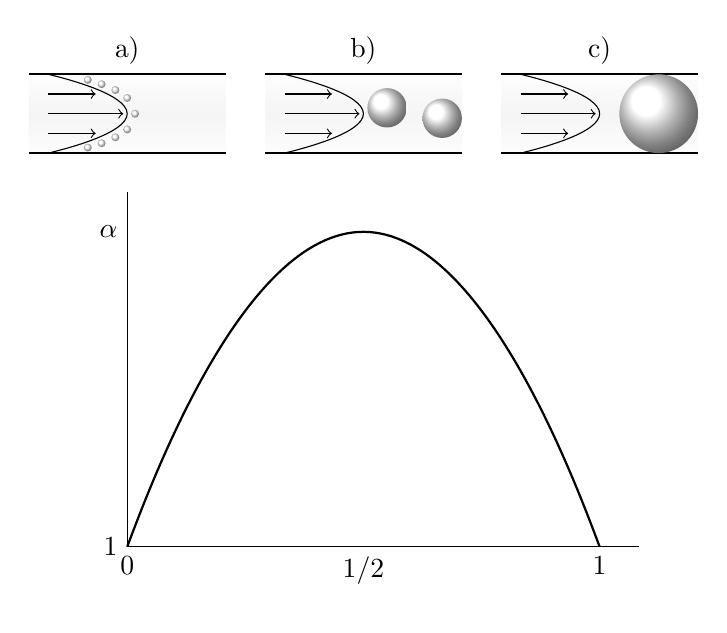
\begin{tikzpicture}

%\draw[help lines] (0,0) grid (12,11);
%\draw (0,-1)--(12,-1)--(12,11)--(0,11)--cycle;
\node[above] at (3,6) {a)};
\node[above] at (6,6) {b)};
\node[above] at (9,6) {c)};
%
%\begin{scope}[very thick]
%\draw (2,10)--(2,5);
%\draw (4,10)--(4,5);
%
%\draw (5,10)--(5,5);
%\draw (7,10)--(7,5);
%
%\draw (8,10)--(8,5);
%\draw (10,10)--(10,5);
%\end{scope}
%
%%\draw (2,9.5) parabola (4,9.5);% parabola (4,9.5);
%\draw (2,9.5) parabola bend (3,8)  (4,9.5);
%\draw (5,9.5) parabola bend (6,8)  (7,9.5);
%\draw (8,9.5) parabola bend (9,8)  (10,9.5);
%
%\begin{scope}[yshift=-0.2cm]
%\shade [ball color=white] (2.25,8.59375) circle [radius=0.075cm];
%\shade [ball color=white] (2.5,8.125) circle [radius=0.075cm];
%\shade [ball color=white] (2.75,7.84375) circle [radius=0.075cm];
%\shade [ball color=white] (3,7.75) circle [radius=0.075cm];	
%\shade [ball color=white] (3.75,8.59375) circle [radius=0.075cm];
%\shade [ball color=white] (3.5,8.125) circle [radius=0.075cm];
%\shade [ball color=white] (3.25,7.84375) circle [radius=0.075cm];
%\end{scope}
%
%\draw [->] (2.25,9.5)--(2.25,9.09375);
%\draw [->] (2.5,9.5)--(2.5,8.625);
%\draw [->] (2.75,9.5)--(2.75,8.34375);
%\draw [->] (3,9.5)--(3,8.25);	
%\draw [->] (3.75,9.5)--(3.75,9.09375);
%\draw [->] (3.5,9.5)--(3.5,8.625);
%\draw [->] (3.25,9.5)--(3.25,8.34375);
%
%\begin{scope}[xshift=3cm]
%\draw [->] (2.25,9.5)--(2.25,9.09375);
%\draw [->] (2.5,9.5)--(2.5,8.625);
%\draw [->] (2.75,9.5)--(2.75,8.34375);
%\draw [->] (3,9.5)--(3,8.25);	
%\draw [->] (3.75,9.5)--(3.75,9.09375);
%\draw [->] (3.5,9.5)--(3.5,8.625);
%\draw [->] (3.25,9.5)--(3.25,8.34375);
%\end{scope}
%
%\begin{scope}[xshift=6cm]
%\draw [->] (2.25,9.5)--(2.25,9.09375);
%\draw [->] (2.5,9.5)--(2.5,8.625);
%\draw [->] (2.75,9.5)--(2.75,8.34375);
%\draw [->] (3,9.5)--(3,8.25);	
%\draw [->] (3.75,9.5)--(3.75,9.09375);
%\draw [->] (3.5,9.5)--(3.5,8.625);
%\draw [->] (3.25,9.5)--(3.25,8.34375);
%\end{scope}
%
%\shade [ball color=white] (5.75,7.25) circle [radius=0.5cm];
%\shade [ball color=white] (6.25,6) circle [radius=0.5cm];
%
%\shade [ball color=white] (9,6.5) circle [radius=1cm];
\shade[top color=black!1!white, bottom color=black!4!white] (1.75,6) rectangle (4.25,5.5);
\shade[top color=black!4!white, bottom color=black!1!white] (1.75,5) rectangle (4.25,5.5);
\begin{scope}[xshift=3cm]
\shade[top color=black!1!white, bottom color=black!4!white] (1.75,6) rectangle (4.25,5.5);
\shade[top color=black!4!white, bottom color=black!1!white] (1.75,5) rectangle (4.25,5.5);
\end{scope}
\begin{scope}[xshift=6cm]
\shade[top color=black!1!white, bottom color=black!4!white] (1.75,6) rectangle (4.25,5.5);
\shade[top color=black!4!white, bottom color=black!1!white] (1.75,5) rectangle (4.25,5.5);
\end{scope}


%\draw[thick,color=white,pattern=custom north west lines,hatchspread=9pt,hatchthickness=0.5pt] 
%(1.75,4.85)rectangle(4.25,5);
%\draw[thick,color=white,pattern=custom north west lines,hatchspread=9pt,hatchthickness=0.5pt] 
%(1.75,6)rectangle(4.25,6.15);
%\begin{scope}[xshift=3cm]
%\draw[thick,color=white,pattern=custom north west lines,hatchspread=9pt,hatchthickness=0.5pt] 
%(1.75,4.85)rectangle(4.25,5);
%\draw[thick,color=white,pattern=custom north west lines,hatchspread=9pt,hatchthickness=0.5pt] 
%(1.75,6)rectangle(4.25,6.15);
%\end{scope}
%\begin{scope}[xshift=6cm]
%\draw[thick,color=white,pattern=custom north west lines,hatchspread=9pt,hatchthickness=0.5pt] 
%(1.75,4.85)rectangle(4.25,5);
%\draw[thick,color=white,pattern=custom north west lines,hatchspread=9pt,hatchthickness=0.5pt] 
%(1.75,6)rectangle(4.25,6.15);
%\end{scope}

\draw (3,4.5)--(3,0)--(9.5,0);
\draw[thick] (3,0) parabola bend (6,4) (9,0);
\node[left] at (3,4) {$\alpha$};
\node[below] at (3,0) {0};
\node[below] at (6,0) {$1/2$};
\node[below] at (9,0) {1};
\node[left] at (3,0) {1};
\node[below] at (6,-0.5) {$\lambdas$};



\draw[thick] (1.75,5)--(4.25,5) (1.75,6)--(4.25,6);
%\draw[thick] (1.75,4.75)--(1.75,5)--(4.25,5)--(4.25,4.74) (1.75,6.25)--(1.75,6)--(4.25,6)--(4.25,6.25);
\begin{scope}[xshift=3cm]
\draw[thick] (1.75,5)--(4.25,5) (1.75,6)--(4.25,6);
\end{scope}
\begin{scope}[xshift=6cm]
\draw[thick] (1.75,5)--(4.25,5) (1.75,6)--(4.25,6);
\end{scope}
\draw[rotate around={90:(2.5,5.5)}] (2,6) parabola bend (2.5,5) (3,6);
\shade [ball color=white] (3.1,5.5) circle [radius=0.05cm];
\shade [ball color=white] (3,5.7) circle [radius=0.05cm];
\shade [ball color=white] (3,5.3) circle [radius=0.05cm];
\shade [ball color=white] (2.85,5.8) circle [radius=0.05cm];
\shade [ball color=white] (2.85,5.2) circle [radius=0.05cm];
\shade [ball color=white] (2.675,5.875) circle [radius=0.05cm];
\shade [ball color=white] (2.675,5.125) circle [radius=0.05cm];
\shade [ball color=white] (2.5,5.93) circle [radius=0.05cm];
\shade [ball color=white] (2.5,5.07) circle [radius=0.05cm];
\draw[->] (2,5.75)--(2.6,5.75);
\draw[->] (2,5.5)--(2.95,5.5);
\draw[->] (2,5.25)--(2.6,5.25);

\begin{scope}[yshift=-1cm]
\draw[rotate around={90:(5.5,6.5)}] (5,7) parabola bend (5.5,6) (6,7);
\shade [ball color=white] (6.3,6.575) circle [radius=0.25cm];
\shade [ball color=white] (7,6.4425) circle [radius=0.25cm];
\begin{scope}[xshift=3cm,yshift=1cm]
\draw[->] (2,5.75)--(2.6,5.75);
\draw[->] (2,5.5)--(2.95,5.5);
\draw[->] (2,5.25)--(2.6,5.25);
\end{scope}
\end{scope}

\draw[rotate around={90:(8.5,5.5)}] (8,6) parabola bend (8.5,5) (9,6);
\shade [ball color=white] (9.75,5.5) circle [radius=0.5cm];
\begin{scope}[xshift=6cm]
\draw[->] (2,5.75)--(2.6,5.75);
\draw[->] (2,5.5)--(2.95,5.5);
\draw[->] (2,5.25)--(2.6,5.25);
\end{scope}







\end{tikzpicture}
	\caption[Variação da seletividade convectiva em função de \lambdas]{Ilustração da variação da seletividade convectiva em função de \lambdas. a) Quando o soluto apresenta um 
tamanho muito inferior ao do poro ($\lambdas\rightarrow 0$), o soluto pode ocupar praticamente todas as posições radiais e assim adquirir uma velocidade convectiva próxima da do solvente ($\alpha\rightarrow 1$). b) Nesta situação, o soluto tem um raio que é metade do raio do poro ($\lambdas=1/2$). Como o soluto só poderá ocupar posições radias que distem no mínimo $\raioporo/2$ das paredes, o soluto tende a ocupar posições mais centrais, adquirindo assim uma velocidade convectiva superior à velocidade média do solvente. c) Quando o raio do soluto é igual ao raio do poro, ele move-se como se de um pistão se tratasse, adquirindo novamente uma velocidade convectiva igual à do solvente, sendo a seletividade convectiva de novo igual a 1.}
	\label{fig:KceAlpha}
\end{figure} 
Após o referido, a equação~\ref{eq:mssimples} pode assim ser reescrita para a situação ilustrada na figura~\ref{fig:modelohindered}:
\begin{equation}
   	\label{eq:mshindered}
   	-\ctegases T\frac{d\ln x}{dy}=K\atrito_\infty(w-\alpha\fluxoporo)
   \end{equation}   
onde \fluxoporo\ é o fluxo volumétrico de solvente no interior do poro, dado pela equação~\ref{eq:fluxoporo}. 
\index{fluxo!poro}
Multiplicando a equação anterior pela concentração do soluto no interior do poro, $c$, e rearranjando obtém-se:\index{concentração!poro}
\begin{equation}
	\label{eq:mshin2}
	n=-K^{-1}\dinf\frac{dc}{dy}+\alpha\fluxoporo c
\end{equation}
onde $n$ é o fluxo de soluto no poro ($=cw$). 
\index{fluxo!de soluto no poro}
Esta equação assume a mesma forma da equação que se obtém pelo modelo hidrodinâmico de Deen, de onde se pode concluír que:
\begin{equation}
\begin{split}
	\label{eq:kdkkcalfa}
	K^{-1} & =  \kapade \\
	\alpha  & =  \kapace
\end{split}
\end{equation}
onde \kapade\ e \kapace\ são os parâmetros hidrodinâmicos que contabilizam o efeito do transporte restringido na difusão e na convecção respetivamente. 
\index{coeficiente!de impedimento convectivo}\index{fator!de impedimento convectivo|see{coeficiente}}%
\index{coeficiente!de impedimento difusivo}\index{fator!de impedimento difusivo|see{coeficiente}}%
Interessa salientar que todas as variáveis presentes na equação~\ref{eq:mshin2} são médias radiais, pelo que a concentração de soluto no interior do poro é apenas função de $y$.
\index{media@média radial}
Os parâmetros \kapade\ e \kapace\ podem ser determinados por correlações existentes na literatura \cite{dechadilok} obtidas pelo modelo hidrodinâmico, para solutos esféricos neutros e em poros cilíndricos:
\begin{equation}
\label{eq:dechadilok}
	\begin{split}
\kapade = {} & (1-\lambdas)^{-2}\left(1+\frac{9}{8}\lambdas\ln\lambdas-1.56034\lambdas+0.528255\lambdas^2+1.91521\lambdas^3-2.81903\lambdas^4\right. \\
& \left.\vphantom{\frac{9}{8}}+0.270788\lambdas^5+1.10115\lambdas^6-0.435933\lambdas^7\right) \\
\kapace = {} & \left( \frac{1+3.867\lambdas-1.907\lambdas^2-0.834\lambdas^3}{1+1.867\lambdas-0.741\lambdas^2}\right)
	\end{split}
\end{equation}
Na figura~\ref{fig:kdekc} encontra-se a representação gráfica dos parâmetros da equação anterior. O parâmetro $\kapade$ tende para zero à medida que $\lambdas$ tende para 1. O significado físico deste parâmetro é o rácio entre o coeficiente de atrito numa solução não confinada e esse mesmo coeficiente de atrito no interior do poro (equação~\ref{eq:K} e equação~\ref{eq:kdkkcalfa}), o que significa que à medida que o valor de $\lambdas$ aumenta, o coeficiente de atrito no interior do poro é consideravelmente superior ao coeficiente que se obtém na mesma solução não confinada, e tende para infinito à medida que \lambdas\ tende para 1. A variação de $\kapace$ reflete o comportamento da seletividade convectiva discutido anteriormente. 
\begin{figure}
\centering
%!TEX root=testfigumV2.tex

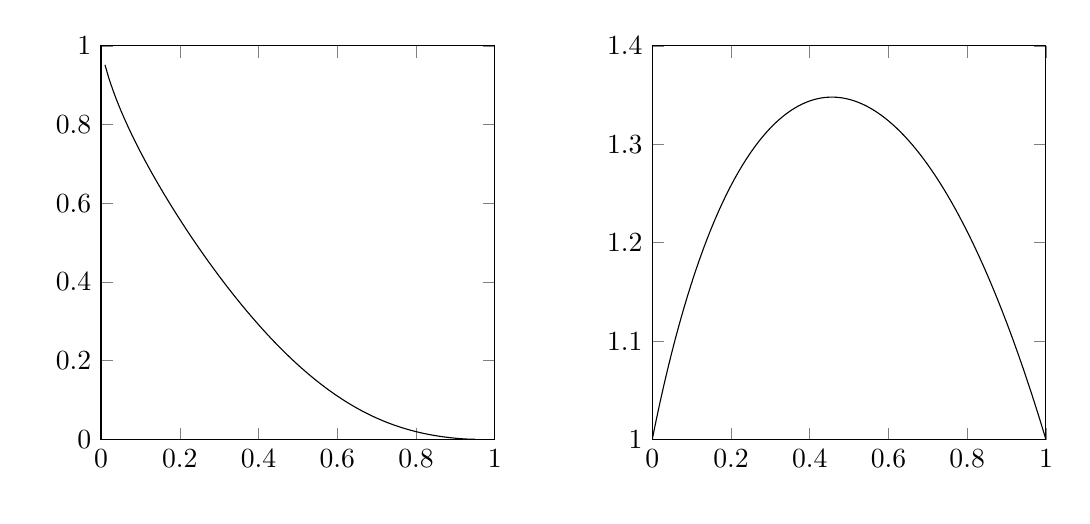
\begin{tikzpicture}

%\draw[help lines] (0,0) grid (14,6);

\begin{axis}[%
width=5cm,
height=5cm,
unbounded coords=jump,
scale only axis,
xmin=0,
xmax=1,
xlabel={$\lambdas$},
ymin=0,
ymax=1,
ylabel={$\kapade$},
name=plot1
]
\addplot [
color=black,
solid,
forget plot
]
table[row sep=crcr]{
0.01 0.951579571426905\\
0.02 0.917324881246881\\
0.03 0.887839563284625\\
0.04 0.861216823754025\\
0.05 0.836582084112171\\
0.06 0.813437240911688\\
0.07 0.79146403605473\\
0.08 0.770443881024649\\
0.09 0.750219004320101\\
0.1 0.730671357376383\\
0.11 0.711710190874481\\
0.12 0.693264273395862\\
0.13 0.675276776599045\\
0.14 0.65770177939606\\
0.15 0.640501800389034\\
0.16 0.623646008215639\\
0.17 0.607108893120014\\
0.18 0.590869260892101\\
0.19 0.574909457438117\\
0.2 0.559214761749886\\
0.21 0.543772904065311\\
0.22 0.52857367859903\\
0.23 0.513608628742172\\
0.24 0.498870788515723\\
0.25 0.484354468203076\\
0.26 0.470055075049459\\
0.27 0.455968962066875\\
0.28 0.442093299566625\\
0.29 0.428425965221866\\
0.3 0.41496544935285\\
0.31 0.401710772805939\\
0.32 0.388661415319784\\
0.33 0.375817252677794\\
0.34 0.363178501263873\\
0.35 0.350745668889511\\
0.36 0.338519510960044\\
0.37 0.326500991208\\
0.38 0.31469124635052\\
0.39 0.303091554132673\\
0.4 0.291703304303973\\
0.41 0.280527972145685\\
0.42 0.269567094224428\\
0.43 0.258822246095658\\
0.44 0.248295021720718\\
0.45 0.237987014394646\\
0.46 0.227899799010209\\
0.47 0.218034915507448\\
0.48 0.208393853378281\\
0.49 0.198978037112984\\
0.5 0.189788812490124\\
0.51 0.180827433624274\\
0.52 0.172095050696855\\
0.53 0.163592698304999\\
0.54 0.155321284371802\\
0.55 0.147281579568694\\
0.56 0.139474207207344\\
0.57 0.131899633564459\\
0.58 0.124558158608382\\
0.59 0.117449907101475\\
0.6 0.110574820057226\\
0.61 0.103932646535763\\
0.62 0.097522935766344\\
0.63 0.0913450295904154\\
0.64 0.0853980552242643\\
0.65 0.0796809183463124\\
0.66 0.0741922965210726\\
0.67 0.0689306329798897\\
0.68 0.0638941307885996\\
0.69 0.0590807474443521\\
0.7 0.0544881899594246\\
0.71 0.050113910509534\\
0.72 0.0459551027499902\\
0.73 0.0420086989369224\\
0.74 0.0382713680363478\\
0.75 0.0347395150650183\\
0.76 0.0314092819914238\\
0.77 0.0282765506418346\\
0.78 0.0253369482208868\\
0.79 0.0225858562904048\\
0.8 0.02001842439028\\
0.81 0.017629589985553\\
0.82 0.0154141071746279\\
0.83 0.0133665877413563\\
0.84 0.0114815599269562\\
0.85 0.00975355316717256\\
0.86 0.00817722175302306\\
0.87 0.00674752835054469\\
0.88 0.00546002227260038\\
0.89 0.00431127277587461\\
0.9 0.00329956587510615\\
0.91 0.00242606960645416\\
0.92 0.00169687760731129\\
0.93 0.00112680929760381\\
0.94 0.000747016002204206\\
0.95 0.000621721294979948\\
};
\end{axis}

\begin{axis}[%
width=5cm,
height=5cm,
scale only axis,
xmin=0,
xmax=1,
xlabel={$\lambdas$},
ymin=1,
ymax=1.4,
ylabel={$\kapace$},
at={(7cm,0cm)},
anchor=south west,
]
\addplot [
color=black,
solid,
forget plot
]
table[row sep=crcr]{
0 1\\
0.01 1.01951958180864\\
0.02 1.03811501078643\\
0.03 1.05583784268832\\
0.04 1.07273538082732\\
0.05 1.08885109677301\\
0.06 1.10422500190201\\
0.07 1.11889397636734\\
0.08 1.13289206106913\\
0.09 1.14625071738811\\
0.1 1.15899905875569\\
0.11 1.17116405755615\\
0.12 1.18277073036938\\
0.13 1.19384230415032\\
0.14 1.20440036559142\\
0.15 1.21446499561691\\
0.16 1.22405489070369\\
0.17 1.23318747250622\\
0.18 1.24187898707642\\
0.19 1.250144594809\\
0.2 1.25799845210454\\
0.21 1.26545378562282\\
0.22 1.27252295989543\\
0.23 1.27921753897663\\
0.24 1.28554834273328\\
0.25 1.29152549830598\\
0.26 1.29715848721449\\
0.27 1.30245618852758\\
0.28 1.30742691847204\\
0.29 1.31207846681512\\
0.3 1.3164181303192\\
0.31 1.32045274353609\\
0.32 1.32418870718083\\
0.33 1.32763201430024\\
0.34 1.3307882744298\\
0.35 1.3336627359132\\
0.36 1.33626030654157\\
0.37 1.33858557265433\\
0.38 1.34064281682983\\
0.39 1.34243603428178\\
0.4 1.34396894806662\\
0.41 1.34524502319722\\
0.42 1.34626747974934\\
0.43 1.34703930503985\\
0.44 1.34756326494807\\
0.45 1.34784191444576\\
0.46 1.34787760739505\\
0.47 1.34767250566883\\
0.48 1.34722858764313\\
0.49 1.34654765610701\\
0.5 1.34563134563135\\
0.51 1.34448112943472\\
0.52 1.34309832578131\\
0.53 1.34148410394265\\
0.54 1.33963948975294\\
0.55 1.33756537078462\\
0.56 1.33526250116924\\
0.57 1.33273150608649\\
0.58 1.32997288594229\\
0.59 1.32698702025545\\
0.6 1.32377417127072\\
0.61 1.32033448731469\\
0.62 1.31666800590976\\
0.63 1.31277465666008\\
0.64 1.30865426392263\\
0.65 1.30430654927512\\
0.66 1.29973113379187\\
0.67 1.29492754013791\\
0.68 1.28989519449053\\
0.69 1.2846334282971\\
0.7 1.27914147987715\\
0.71 1.27341849587602\\
0.72 1.26746353257702\\
0.73 1.26127555707834\\
0.74 1.25485344834044\\
0.75 1.24819599810934\\
0.76 1.24130191172074\\
0.77 1.2341698087893\\
0.78 1.22679822378739\\
0.79 1.21918560651704\\
0.8 1.21133032247841\\
0.81 1.20323065313808\\
0.82 1.19488479609991\\
0.83 1.18629086518103\\
0.84 1.17744689039529\\
0.85 1.16835081784627\\
0.86 1.15900050953151\\
0.87 1.14939374305979\\
0.88 1.13952821128266\\
0.89 1.12940152184147\\
0.9 1.11901119663092\\
0.91 1.10835467117981\\
0.92 1.0974292939498\\
0.93 1.08623232555244\\
0.94 1.07476093788478\\
0.95 1.06301221318378\\
0.96 1.05098314299931\\
0.97 1.03867062708563\\
0.98 1.02607147221091\\
0.99 1.01318239088432\\
1 1\\
};
\end{axis}
\end{tikzpicture}%
\caption[Representação gráfica dos parâmetros $\kapade$ e $\kapace$]{Representação gráfica dos parâmetros $\kapade$ e $\kapace$, em função de $\lambdas$, obtidos pelas correlações representadas na equação~\ref{eq:dechadilok} \cite{dechadilok}.}
\label{fig:kdekc}
\end{figure}

Uma das utilizações mais frequentes do modelo enunciado, que foi também utilizada no presente trabalho, é a caracterização de membranas quanto ao seu tamanho de poro \cite{moraompa,moraotese,moraodes,bowen02}. 
\index{caracterização!membranas}
Para isso, são determinadas as permeações observadas de solutos de referência, geralmente neutros e com geometria aproximadamente esférica, e o raio de poro determinado como sendo o valor que minimiza os erros entre os resultados obtidos e as previsões do modelo. A equação \ref{eq:mshin2}, juntamente com a equação \ref{eq:kdkkcalfa}, pode ser integrada ao longo do poro, obtendo-se após alguma manipulação algébrica:
\begin{equation}
	\label{eq:odkvn}
	n=\kapace\fluxoporo c_0\frac{\left[1-\left(c_L/c_0\right)\euler^{-\peclet}\right]}{1-\euler^{-\peclet}}
\end{equation}
onde \peclet\ é o número de Peclet, dado por:
\begin{equation}
	\label{eq:peclet}
	\peclet=\frac{\kapace\fluxoporo\comporo}{\kapade\dinf}
\end{equation}\index{número!de Peclet}%
As concentrações $c_0$ e $c_L$ podem ser relacionadas com a concentração junto à membrana (\concm) e com a concentração no permeado (\concp), respetivamente, através do coeficiente de partição (equação~\ref{eq:particaohs}). 
\index{coeficiente!de partição}
\index{concentração!no poro}
O fluxo molar de soluto no poro, $n$, pode ser relacionado com o fluxo molar de soluto com base na área total de membrana, $N$, através da porosidade ($N=\porosidade n$). Por seu lado, $N$ é dado pelo produto entre o fluxo de filtração, \fluxo, e a concentração do soluto no permeado ($N=\fluxo\concp$). Assim, o fluxo molar de soluto no poro pode ser obtido por:
\index{fluxo!molar}\index{fluxo!de soluto no poro}\index{porosidade}
\begin{equation}
	\label{eq:fluxoporoaid}
	n=\frac{N}{\porosidade}=\frac{\fluxo\concp}{\porosidade}=\fluxoporo\concp
\end{equation}
Substituindo as equações~\ref{eq:particaohs}~e~\ref{eq:fluxoporoaid} na equação~\ref{eq:odkvn}, obtém-se após alguma manipulação algébrica:
\begin{equation}
	\label{eq:smhindered}
	\permm=\frac{\particao\kapace}{1-(1-\particao\kapace)\euler^{-\peclet}}
\end{equation}\index{permeação!intrínseca}%
onde \permm\ é a permeação intrínseca definida pela equação~\ref{eq:permintr}. O comprimento dos poros, $\comporo$, que figura na equação~\ref{eq:peclet} nem sempre é conhecido com exatidão para uma determinada membrana, sendo a sua determinação por vezes difícil de obter experimentalmente.
\index{comprimento!poro}
Este valor pode ser relacionado com outros parâmetros, mais facilmente determináveis, através da equação de Hagen-Poiseuille (equação~\ref{eq:fluxoporo}). Com o auxílio da equação~\ref{eq:permhidro}, o número de Peclet pode ser definido alternativamente por:
\begin{equation}
	\label{eq:peclet2}
	\peclet=\frac{\kapace\raioporo^2\fluxo}{8\kapade\dinf\permhidra\viscosidade}
\end{equation}\index{número!de Peclet}%
O coeficiente de difusão do soluto (\dinf) pode ainda ser relacionado com o seu raio hidrodinâmico através da equação de Stokes-Einstein (equação~\ref{eq:stokesein}).\footnote{O símbolo $\infty$ é usado para indicar que o coeficiente de difusão, que figura na equação~\ref{eq:peclet2}, é o coeficiente de difusão numa situação não confinada e não esse mesmo coeficiente no interior do poro.} 
\index{coeficiente!de difusão}\index{raio!hidrodinâmico}
Se a polarização de concentração não puder ser desprezada, a permeação observada, \permobs, irá assumir um valor diferente de \permm. Neste caso, a equação~\ref{eq:sobsvssm} pode ser usada para relacionar estes dois parâmetros. O valor de \permobs\ obtido pode assim ser comparado com os resultados experimentais.\index{permeação!observada}
% section restringido (end)

\section{Partição de moléculas longas e flexíveis}
\label{sec:fjcecsc}
Como discutido na secção~\ref{sec:restringido}, se os solutos puderem ser considerados rígidos e com geometria esférica, os coeficientes de partição, que relacionam as concentrações adjacentes à interface solução não-confinada-solução no interior do poro, podem ser facilmente calculados pela equação~\ref{eq:particaohs}. Uma consequência imediata da referida equação é a ausência de permeação no caso de solutos para os quais $\lambdas> 1$. No entanto, observa-se experimentalmente que alguns solutos obedecem relativamente bem à equação~\ref{eq:particaohs}, mas existem outros que exibem consideráveis desvios \cite{dechadilok}. Como referido no capítulo~\ref{chap:intro}, os plasmídeos enquadram-se nesta última categoria. Esta observação experimental indica com clareza que a equação~\ref{eq:particaohs} não pode ser usada neste caso. Sendo os plasmídeos moléculas flexíveis e de elevada massa molecular, a determinação exata dos coeficientes de partição, com base numa representação geométrica rigorosa das moléculas revela-se um problema de excessiva complexidade. Uma forma de conseguir a sua determinação aproximada passa por representar essa mesma estrutura por modelos mais simplificados, que possam ainda assim reter as principais características da molécula que determinam a sua partição nos poros de membranas.   

Um dos modelos de representação de macromoléculas mais simples consiste em considerar o soluto como um cadeia de ligação livre (FJC).\index{FJC}\index{cadeias!de ligação livre|see{FJC}}
Durante a geração de uma FJC, a única imposição passa por manter constante a distância entre vários pontos, podendo os ângulos de ligação assumir qualquer valor \cite{teraoka}. Uma representação FJC pode assim simular a estrutura e conformação de uma macromolécula linear. Os parâmetros que caracterizam uma cadeia FJC são o comprimento dos segmentos, \comsegmento, que assume um valor constante, e o número total de segmentos, \numsegmento. 
\index{comprimento!segmentos}\index{número!segmentos}
Estes segmentos, que se consideram ter massa nula, unem $\numsegmento +1$ massas pontuais. A representação análoga para cadeias circulares, ou fechadas, são as denominadas cadeias segmentadas fechadas (CSC), que podem ser geradas a partir de uma cadeia FJC (secção~\ref{subsec:csc}).\index{CSC}\index{cadeias!fechadas segmentadas|see{CSC}}
Apesar das estruturas simplificadas, FJC e CSC, apresentarem já uma considerável redução da complexidade estrutural das moléculas reais, a determinação do coeficiente de partição é geralmente feita por métodos estocásticos, conhecidos como métodos de Monte-Carlo \cite{davidson87,cifra,hermsen}. 
\index{Monte-Carlo}
Neste tipo de métodos, a estrutura da molécula é gerada e é estabelecida uma condição para a sua entrada no poro. A probabilidade de entrada da molécula no poro é assim determinada testando esta condição um elevado número de vezes.

Nesta secção apresentam-se os métodos usados no presente trabalho para a geração de estruturas FJC e CSC, e para a determinação dos coeficientes de partição, necessários para completar o desenvolvimento teórico. 
%Nesta secção utiliza-se o programa Matlab\registado\ para demonstrar a geração deste tipo de moléculas. 

\subsection{Cadeias de ligação livre (FJC)}
\label{subsec:fjc}\index{FJC}
Numa primeira abordagem, e para facilitar o raciocínio, pode-se considerar o problema de gerar uma cadeia FJC em apenas duas dimensões, ficando posteriormente mais facilitada a abordagem para três dimensões, que será discutida na secção~\ref{subsec:3d}. Uma cadeia FJC pode ser gerada por um caminho aleatório em \numsegmento\ passos. Em cada passo, um novo ponto é gerado, podendo este novo ponto ocupar qualquer posição numa circunferência de raio \comsegmento\ centrada no ponto anterior. O processo é repetido até que a cadeia gerada possua \numsegmento\ segmentos. Em duas dimensões, o problema é simplificado se for utilizado o sistema de coordenadas polares, sendo a sua relação com o sistema cartesiano dado pelas seguintes expressões:\index{coordenadas!cartesianas}\index{coordenadas!polares}
\begin{equation}
\label{eq:polar}
\begin{split}
       x & = r\cos\theta       \\
       y & = r\sin\theta       \\
	     r & = \sqrt{x^2+y^2}    \\
  \theta & = \mr{arctan2}(y,x)
\end{split}
\end{equation}
A função $\mr{arctan2}$ deve ser usada, por substituição da tradicional função $\arctan$, para que o ângulo possa ser determinado inequivocamente. 
\index{arctan2}\index{atan2@\texttt{atan2}}%
Por exemplo, o ângulo $\theta$ entre um vetor $(x,y)$ e o eixo positivo dos $xx$ pode ser obtido por $\arctan(y/x)$. 
\index{vetor}\index{angulo!ângulo}
No entanto, este método não distingue entre vetores diametralmente opostos\footnote{Vetores do tipo $(+x,+y)$ e $(-x,-y)$ não são distinguidos pelo método $\arctan(y/x)$.}. Além disso, vetores com abcissa nula causam problemas pelo facto de $y/x$ não ser um número neste caso. A função $\mr{arctan2}$, definida em muitas linguagens de programação pela função \texttt{atan2}, permite superar estas limitações. Esta função é definida por:
\begin{equation}
\mr{arctan2}(x,y)=\left\{ \begin{array}{ll}%
				\arctan(y/x) 		& \mbox{$x>0$}		\\
				\arctan(y/x)+\pi 	& \mbox{$y\geq0, x<0$}	\\
				\arctan(y/x)-\pi 	& \mbox{$y\leq0, x<0$}	\\
				\pi/2			& \mbox{$y>0, x=0$}	\\
				-\pi/2			& \mbox{$y<0, x=0$}	\\
				\text{não definido}	& \mbox{$x=0, y=0$}	
			         \end{array}    	
			\right.
\end{equation}
Cada ponto $i$ de uma cadeia FJC em duas dimensões é definido pelas suas coordenadas, que representam o seu vetor posição $\vec{r_{i}}$ (ver figura~\ref{fig:rw2d}). Em cada passo, um novo ponto é gerado segundo o vetor $\Delta\vec{r}_{i}$, dado por $\vec{r}_{i+1}-\vec{r}_{i}$. Em coordenadas polares a posição de um novo ponto da cadeia pode assim ser obtida por: 
%
\begin{equation}
\label{eq:xi}
\begin{split}
x_{i+1} & = x_{i}+\comsegmento \cos \theta_{i+1} \\
y_{i+1} & = y_{i}+\comsegmento \sin \theta_{i+1}
\end{split}
\end{equation}
% 
\begin{figure}
	\centering
	\setlength\figureheight{6cm} 
	\setlength\figurewidth{6cm}
	% This file was created by matlab2tikz v0.3.3.
% Copyright (c) 2008--2013, Nico Schlömer <nico.schloemer@gmail.com>
% All rights reserved.
% 
% The latest updates can be retrieved from
%   http://www.mathworks.com/matlabcentral/fileexchange/22022-matlab2tikz
% where you can also make suggestions and rate matlab2tikz.
% 
% 
% 
\begin{tikzpicture}

\begin{axis}[%
width=\figurewidth,
height=\figureheight,
unbounded coords=jump,
clip=false,
scale only axis,
xmin=-2,
xmax=2,
xlabel={$\alpha$},
ymin=-3,
ymax=4,
hide axis
]
\addplot [
color=black,
solid,
mark=*,
mark options={solid,fill=black,draw=black},
forget plot
]
table[row sep=crcr]{
0 0\\
0.927448823450819 -0.373950103462604\\
1.63873197433658 -1.07685570115408\\
0.687979473962849 -1.38680679896322\\
-0.0302557526830962 -2.08260717206233\\
-0.884387140825643 -2.60266444947481\\
-0.6219828094829 -1.63770643645426\\
-0.938437904199134 -0.689098944902491\\
-1.92179572364242 -0.507419559886612\\
-1.79950609012874 0.485074896286867\\
-1.24101999920001 -0.344438989214244\\
-0.90088899493851 0.595939073024588\\
-0.750177536601147 1.58451686780142\\
-0.272327122658547 2.46295809059034\\
-0.132447980529529 3.45312667502293\\
-1.05193722128017 3.84624184408133\\
};

\addplot [fill=black,draw=black,forget plot] table[row sep=crcr]{
0.927448823450819 -0.373950103462604\\
0.757288903712709 -0.209060416421904\\
0.745251759411961 -0.300487709392807\\
0 0\\
0 0\\
0 0\\
0 0\\
0 0\\
0.745251759411961 -0.300487709392807\\
0.733214615111212 -0.391915002363711\\
0.927448823450819 -0.373950103462604\\
};

\addplot [fill=black,draw=black,forget plot] table[row sep=crcr]{
1.63873197433658 -1.07685570115408\\
1.5085816968234 -0.845551624587686\\
1.48335172702006 -0.923305535550613\\
0.927448823450819 -0.373950103462604\\
0.927448823450819 -0.373950103462604\\
0.927448823450819 -0.373950103462604\\
0.927448823450819 -0.373950103462604\\
0.927448823450819 -0.373950103462604\\
1.48335172702006 -0.923305535550613\\
1.45812175721673 -1.00105944651354\\
1.63873197433658 -1.07685570115408\\
};

\addplot [fill=black,draw=black,forget plot] table[row sep=crcr]{
-1.05193722128017 3.84624184408133\\
-0.861217472897483 3.85947890672511\\
-0.873703423189198 3.77004039814461\\
-0.132447980529528 3.45312667502293\\
-0.132447980529528 3.45312667502293\\
-0.132447980529528 3.45312667502293\\
-0.132447980529528 3.45312667502293\\
-0.132447980529528 3.45312667502293\\
-0.873703423189198 3.77004039814461\\
-0.886189373480914 3.68060188956412\\
-1.05193722128017 3.84624184408133\\
};
\node[right, inner sep=0mm, text=black]
at (axis cs:-1.41547277936963, 4.17048710601719, 17.3205080756888) {$\vec{r}_{n_{k}+1}$};
\node[right, inner sep=0mm, text=black]
at (axis cs:1.67908309455587, -1.24498567335244, 17.3205080756888) {$\vec{r}_{3}$};
\node[right, inner sep=0mm, text=black]
at (axis cs:1.16332378223496, -0.422636103151863, 17.3205080756888) {$\Delta\vec{r}_{2}$};
\node[right, inner sep=0mm, text=black]
at (axis cs:0.89971346704871, -0.121776504297995, 17.3205080756888) {$\vec{r}_{2}$};
\node[right, inner sep=0mm, text=black]
at (axis cs:0.292263610315186, 0.0587392550143262, 17.3205080756888) {$\Delta\vec{r}_{1}$};
\node[right, inner sep=0mm, text=black]
at (axis cs:-0.246418338108882, 0.279369627507163, 17.3205080756888) {$\vec{r}_{1}$};
\node[right, inner sep=0mm, text=black]
at (axis cs:-0.0401146131805161, 3.5487106017192, 17.3205080756888) {$\vec{r}_{n_{k}}$};
\node[right, inner sep=0mm, text=black]
at (axis cs:-0.681948424068768, 3.88968481375358, 17.3205080756888) {$\Delta\vec{r}_{n_{k}}$};
\node[right, inner sep=0mm, text=black]
at (axis cs:0.177650429799427, -1.50573065902579, 17.3205080756888) {$l_{k}$};
\end{axis}
\end{tikzpicture}%
	\caption[Trajetória em duas dimensões de uma cadeia FJC]{Trajetória em duas dimensões de uma cadeia FJC com $n_{k}$ segmentos com comprimento $l_{k}$. Na figura estão igualmente representados os vectores $r_{i}$ e $\Delta\vec{r}_{i}$.}
	\label{fig:rw2d}
\end{figure}
onde $x_{i+1}$ e $y_{i+1}$ representam as coordenadas do novo ponto a ser gerado, $x_{i}$ e $y_{i}$ as coordenadas do ponto anterior e $\theta_{i+1}$ o ângulo entre $\Delta\vec{r}_{i}$ e o eixo dos $xx$. Em coordenadas polares a aleatoriedade do processo resume-se à aleatoriedade no valor que este ângulo toma em cada iteração. O código apresentado na figura~\ref{fig:FJCcode} serve como exemplo.
\index{FJC!código}%
A função \texttt{rand} gera números aleatórios entre 0 e 1. 
\index{número!aleatório}\index{rand@\texttt{rand}}%
Na quarta de linha de código (\texttt{r=rand(nk,1)}) são assim gerados \numsegmento\ números aleatórios entre 0 e 1, que serão posteriormente utilizados dentro do ciclo \texttt{for} para obter um ângulo $\theta$ aleatório no intervalo $0\leq\theta\leq2\pi$, em cada iteração, construindo assim um caminho aleatório em duas dimensões. 

\begin{figure}
  \centering
	%!TEX root=testfigum.tex

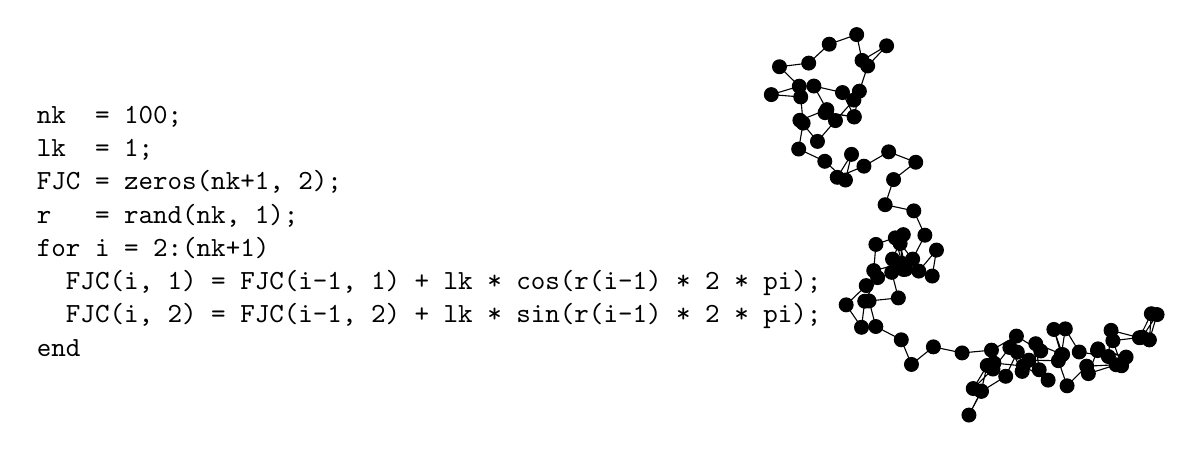
\begin{tikzpicture}

%\draw[help lines] (0,0)grid(14cm,8cm);

% \node[right,align=left] at (0.5,3)
% {\texttt{nk=100;}\\
% \texttt{lk=1;}\\
% \texttt{FJC=zeros(nk+1,2);}\\
% \texttt{r=rand(nk,1);}\\
% \texttt{for i=2:(nk+1)}\\
% \texttt{    FJC(i,1)=FJC(i-1,1)+lk*cos(r(i-1)*2*pi);}\\
% \texttt{    FJC(i,2)=FJC(i-1,2)+lk*sin(r(i-1)*2*pi);}\\
% \texttt{end}};

\node[right,align=left] at (-1,3)
{\texttt{nk~~=~100;}\\
\texttt{lk~~=~1;}\\
\texttt{FJC~=~zeros(nk+1,~2);}\\
\texttt{r~~~=~rand(nk,~1);}\\
\texttt{for~i~=~2:(nk+1)}\\
\texttt{~~FJC(i,~1)~=~FJC(i-1,~1)~+~lk~*~cos(r(i-1)~*~2~*~pi);}\\
\texttt{~~FJC(i,~2)~=~FJC(i-1,~2)~+~lk~*~sin(r(i-1)~*~2~*~pi);}\\
\texttt{end}};


\begin{axis}[%
width=6cm,
height=6cm,
scale only axis,
xmin=-4,
xmax=12,
ymin=-14,
ymax=4,
at={(8cm,0cm)},
anchor=south west,
hide axis
]
\addplot [
color=black,
solid,
mark size=2.5pt,
mark=*,
mark options={solid,fill=black},
forget plot
]
table[row sep=crcr]{
0 0\\
-0.623650435612179 -0.781703354323582\\
-1.23366317338174 -1.57409496190085\\
-1.82837831480844 -0.770158459086218\\
-0.914912134479426 -0.363243802929519\\
-1.35473999284461 0.534838295214018\\
-0.386146008133489 0.286190566928726\\
0.01189315547449 -0.631177856461931\\
-0.976644625403326 -0.480204164127264\\
0.00979661851757174 -0.644318978485358\\
0.186462079552728 0.339951977541099\\
0.466941720731259 1.29981195216467\\
1.10810031475684 2.06722035536804\\
0.276563945575714 1.51175004407402\\
0.0949586641191357 2.49512155156601\\
-0.835508923934372 2.12874733361135\\
-1.52949350906954 1.40875747563086\\
-2.51981122226224 1.26993807159533\\
-1.84908350551731 0.528234404360144\\
-2.79670709506351 0.20884509249205\\
-1.80069695349557 0.119604978788559\\
-1.71899009879385 -0.877051426345503\\
-1.86958209720529 -1.8656474257378\\
-0.985023174918595 -2.33207589078147\\
-0.285248458729725 -3.04643948628644\\
-0.079557043978177 -2.06782258376661\\
-0.565299403918798 -2.94192461428669\\
0.340682611964049 -2.51860843588471\\
1.1776419785464 -1.97134340074171\\
2.09530939010675 -2.36869277064194\\
1.34377319062631 -3.02838462360853\\
1.05753470835865 -3.98654302975498\\
2.02965444254369 -4.22102804507154\\
2.4046050726603 -5.14807282552994\\
1.99089126910619 -6.05847981624826\\
1.4028945851438 -5.24961647819341\\
1.63371164741892 -6.22261364353496\\
0.672180320715843 -6.49730894340123\\
0.745641332539554 -5.50001085368991\\
1.67333335319965 -5.12666447992476\\
1.30903818336818 -6.05794801850872\\
2.19817215645479 -6.5155950199227\\
2.79702814767041 -5.71473829004828\\
2.65296353976311 -6.70430657407344\\
1.68419074212999 -6.45635644488192\\
1.56609900670224 -5.46335375504485\\
1.75160129181897 -6.44599758788382\\
0.803282020830229 -6.7633153470329\\
0.366876369026159 -7.66306537180281\\
0.257991964832806 -8.65711979009361\\
-0.26093711104736 -7.80230249136472\\
0.417719731862983 -7.06784698585675\\
1.28143704140114 -6.56387038996745\\
1.5066538915936 -7.53817905275835\\
0.513322245226698 -7.65347103134324\\
0.742926090272591 -8.6267552007101\\
1.6053294065606 -9.13297700985649\\
1.94982894173496 -10.0717634979701\\
2.69250620431969 -9.40211397498089\\
3.6654092813168 -9.63332730238561\\
4.65982842706223 -9.52782582099821\\
5.50426870824634 -8.99217611128701\\
6.32757181192001 -9.55977808404724\\
5.69854998575414 -10.3371657236499\\
5.28270228615632 -9.4277314540409\\
4.71002673020161 -10.2475135638798\\
4.04140336372726 -10.9911147969372\\
4.51696200771091 -10.1114307763182\\
4.30851184138869 -11.0894637656188\\
3.89701615536808 -12.0008754730192\\
4.32212765167401 -11.095734480848\\
5.14206008352864 -10.5232741702649\\
5.53474317396723 -9.60360032020521\\
6.27545221893694 -10.2754262728894\\
6.15810443406316 -9.28233539216137\\
7.06945430203664 -9.69396801738042\\
6.7726742092411 -8.73902216733431\\
7.02449753189967 -9.70679539188911\\
7.16083931256247 -8.71613353290508\\
7.6324316039259 -9.5979502432971\\
8.61760172366452 -9.76953064769742\\
8.70964493132775 -8.77377563368892\\
9.66967334014742 -9.05367821363268\\
10.0745998464419 -8.13932897811043\\
10.0080279829066 -9.13711061102689\\
10.2680972387977 -8.17152064518205\\
9.76293472789264 -9.03454488445699\\
8.77169334969824 -9.16660748383799\\
9.06583674973066 -10.1223687826032\\
8.24961599522573 -9.54462863347438\\
9.21859869623736 -9.79175719341881\\
8.26911154562037 -9.4779512807702\\
7.94116751625036 -10.4226484352068\\
8.88233006552947 -10.0846942136997\\
7.88378018981732 -10.1385286424165\\
7.22006182774944 -10.886511219656\\
6.92649296938934 -9.93057328997589\\
5.92669424332487 -9.91051070390488\\
6.57775910952512 -10.6695327984447\\
5.73516012692558 -10.1309912916672\\
4.74141876992816 -10.0192858066053\\
};
\end{axis}

\end{tikzpicture}
\caption[Código \textsc{Matlab}\textsuperscript{\textregistered}/GNU Octave para gerar uma FJC]{Código \textsc{Matlab}\textsuperscript{\textregistered}/GNU Octave para gerar uma FJC com $\protect\numsegmento = 100$ e $\protect\comsegmento = 1$, com a respetiva representação gráfica do resultado.}
\label{fig:FJCcode}
\end{figure}

As dimensões de uma cadeia FJC podem ser definidas por duas variáveis: a distância média entre as suas extremidades, \distanciah, e o raio de giração médio, normalmente designado apenas por raio de giração, \raiogiracao\ \cite{teraoka}. 
\index{distância!entre extremidades de uma cadeia}\index{raio!de giração}
Devido à aleatoriedade no valor de $\theta$, cada geração de uma cadeia FJC com o código apresentado na figura~\ref{fig:FJCcode} produz uma cadeia com dimensões diferentes. Para estimar uma dimensão média de uma cadeia FJC é assim preciso gera-la um elevado número de vezes, calculando em cada geração a distância entre as suas extremidades, $h$, e o raio de giração instantâneo, $\raiogiracao^{*}$:

\begin{equation}
\label{eq:herg}
\begin{split}
  h & = \left|\vec{r}_{n_{k}+1}-\vec{r}_{1}\right|  \\
  (\raiogiracao^{*})^{2} & = \frac{1}{n_{k}+1}\sum_{i=1}^{n_{k}+1}\left(\vec{r}_{i}-\vec{r}_{\mr{cm}}\right)^{2}
\end{split}
\end{equation}
As coordenadas do centro de massa da molécula, $\vec{r}_{\mr{cm}}$, considerando todas as massas pontuais com igual massa, podem ser dadas por:\index{coordenadas!do centro de massa}
\begin{equation}
\label{eq:centromassa}
\vec{r}_{\mr{cm}}=\frac{1}{\numsegmento+1}\sum_{i=1}^{\numsegmento+1} \vec{r}_{i}
\end{equation}

\subsection{Cadeias fechadas segmentadas (CSC)}
\label{subsec:csc}\index{CSC}\index{pDNA|see{DNA plasmídico}}
Os plasmídeos, na sua forma nativa, são moléculas circulares, ao contrário de uma cadeia FJC, que é por natureza uma cadeia aberta. Para superar esta limitação, é proposto neste trabalho uma nova estrutura de cadeia fechada, denominada cadeia fechada segmentada (CSC). Esta nova estrutura pode ser considerada a análoga de uma estrutura FJC mas com conformação circular (ou fechada). De facto, para gerar uma CSC é necessário gerar primeiro a FJC correspondente. Utilizando de novo coordenadas polares, o código representado na figura~\ref{fig:csc_vs_fjc} pode ser usado para gerar uma cadeia CSC. 
\index{CSC!código}
Como se pode ver na figura, a estrutura CSC obtida é agora uma cadeia aleatória fechada, que ainda assim se assemelha naturalmente à cadeia FJC correspondente.

O algoritmo para gerar uma cadeia CSC, a partir de uma FJC, é o seguinte: após gerar a cadeia FJC o seu vetor $\vec{r}_{\numsegmento+1}$ é feito coincidir com o vetor $\vec{r}_{1}$. 
\index{CSC!algoritmo}
Em seguida, o vetor $\vec{r}_{\numsegmento}$ é movido até ficar à distância \comsegmento\ pretendida, segundo a direção do vetor $\Delta\vec{r}_{\numsegmento}$ ($=\vec{r}_{\numsegmento}-\vec{r}_{\numsegmento+1}$). De seguida, o vetor $\vec{r}_{\numsegmento-1}$ é movido até ficar a uma distância \comsegmento\ do vetor $\vec{r}_{\numsegmento}$, segundo a direção do vetor $\Delta\vec{r}_{\numsegmento-1}$, e assim sucessivamente.
%
\begin{figure}[!t]
	\centering
	%!TEX root=testfigum.tex
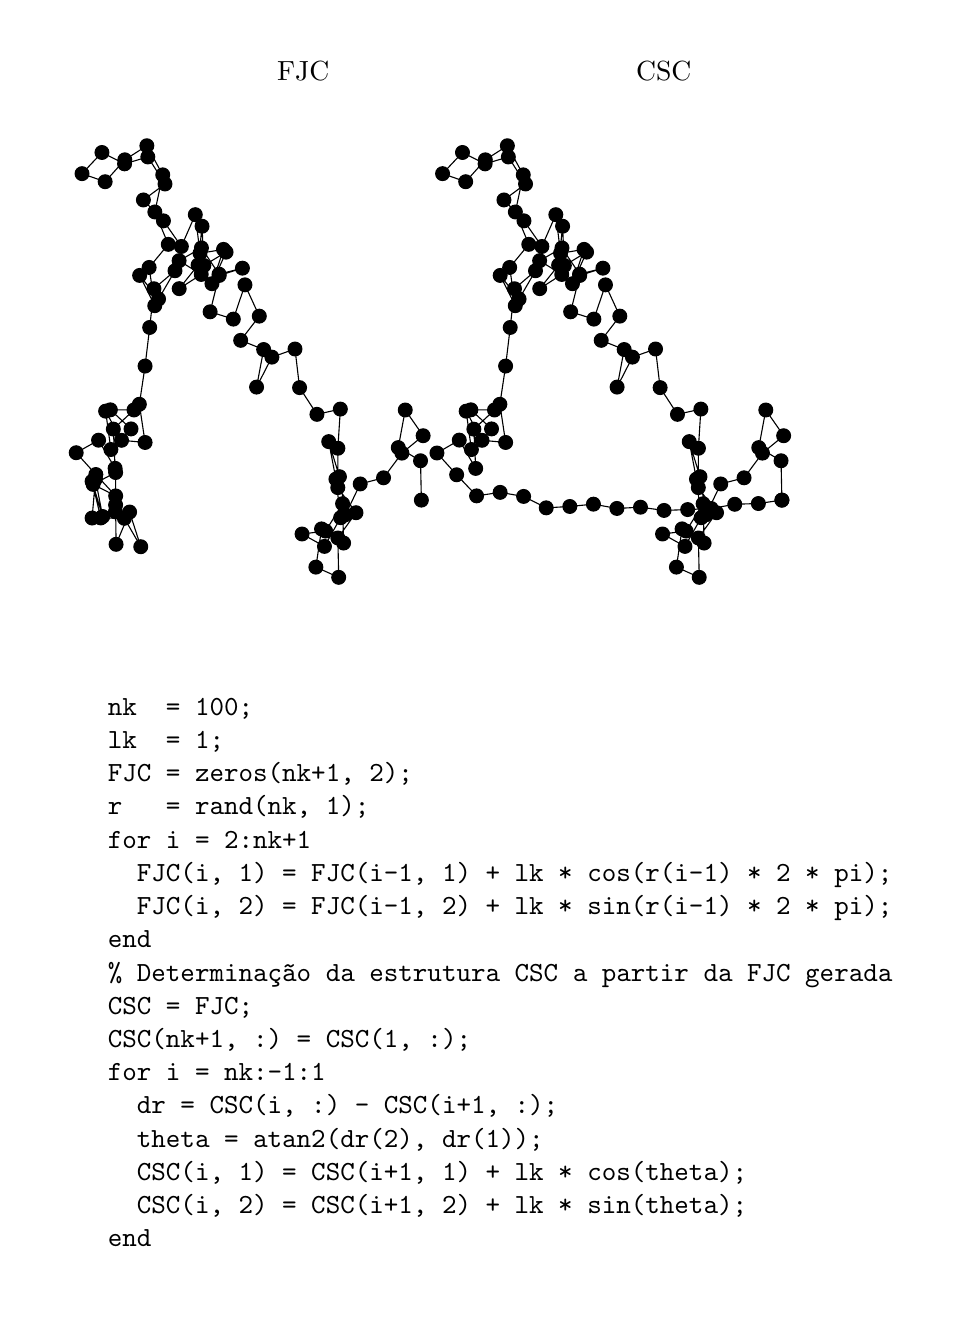
\begin{tikzpicture}
\useasboundingbox (-0.5cm,-9.3cm)rectangle(11cm,7cm);

\node[align=left] at (5.5,-5)
{\texttt{nk~~=~100;}\\
\texttt{lk~~=~1;}\\
\texttt{FJC~=~zeros(nk+1,~2);}\\
\texttt{r~~~=~rand(nk,~1);}\\
\texttt{for~i~=~2:nk+1}\\
\texttt{~~FJC(i,~1)~=~FJC(i-1,~1)~+~lk~*~cos(r(i-1)~*~2~*~pi);}\\
\texttt{~~FJC(i,~2)~=~FJC(i-1,~2)~+~lk~*~sin(r(i-1)~*~2~*~pi);}\\
\texttt{end}\\
\texttt{\% Determinação da estrutura CSC a partir da FJC gerada}\\
\texttt{CSC~=~FJC;}\\
\texttt{CSC(nk+1,~:)~=~CSC(1,~:);}\\
\texttt{for~i~=~nk:-1:1}\\
\texttt{~~dr~=~CSC(i,~:)~-~CSC(i+1,~:);}\\
\texttt{~~theta~=~atan2(dr(2),~dr(1));}\\
\texttt{~~CSC(i,~1)~=~CSC(i+1,~1)~+~lk~*~cos(theta);}\\
\texttt{~~CSC(i,~2)~=~CSC(i+1,~2)~+~lk~*~sin(theta);}\\
\texttt{end}};

\begin{axis}[%
width=6cm,
height=6cm,
scale only axis,
xmin=-15,
xmax=5,
ymin=-2,
ymax=10,
hide axis,
name=plot1,
title={FJC}
]
\addplot [
color=black,
solid,
mark size=2.5pt,
mark=*,
mark options={solid,fill=black},
forget plot
]
table[row sep=crcr]{
0 0\\
-0.0359534635777112 0.999353465224775\\
-0.978413588767783 1.33367204446726\\
-0.682563623554148 2.28890646495424\\
0.0743410317518025 1.63538114579959\\
-0.822779558153791 1.19359539776392\\
-1.60185411386996 0.566664112346087\\
-2.58958093309086 0.410472785468583\\
-3.21242935959367 -0.371869746676369\\
-3.4682027505772 0.594867018148879\\
-3.92251271833553 1.48571069309719\\
-3.61727552296498 0.533434339005424\\
-3.41803667700261 -0.446516620104053\\
-4.10263398079752 -1.17543810533874\\
-5.05179832692601 -0.860657159221478\\
-4.05455321028174 -0.78648049625289\\
-3.33567146462779 -0.0913481090304791\\
-3.29276403527912 -1.09042716121138\\
-4.22594862074044 -0.731029707885157\\
-4.46591120926599 -1.70181184415885\\
-3.50016560408655 -1.96130254934228\\
-3.53488085782371 -0.961905305420741\\
-2.76782198746937 -0.320328584045413\\
-3.5380492693521 0.317440915259413\\
-3.53412746134844 1.31743322494083\\
-3.43014014320752 2.31201184811039\\
-4.42121260608284 2.17868753176018\\
-5.1560384502441 2.85694336752771\\
-5.34954726604928 3.8380419039682\\
-6.32803532352806 3.63173843484709\\
-6.97677529019789 2.8707282800888\\
-6.67717797514429 3.82479402667689\\
-7.64962357258638 4.05792394756972\\
-6.86124866924489 4.67311904815269\\
-7.46839534199571 5.46770882770413\\
-7.9604893881869 4.59716678408809\\
-8.94312007549804 4.78273869024423\\
-8.55915124270638 5.70608474424816\\
-7.57646373852119 5.89135554366962\\
-8.56479052075719 5.73900669557737\\
-9.31065128758991 6.40510857704874\\
-10.256680678743 6.08102773671031\\
-9.31961387957932 5.73187760581373\\
-10.2522239939527 5.37099206361449\\
-9.45187561832646 5.97052728162291\\
-9.28495279843158 6.95649724678328\\
-9.2093156055953 5.95936184220683\\
-8.26863555033685 6.29865674879838\\
-8.8659866356463 5.49667689812903\\
-8.37600185497933 6.36840788571335\\
-9.37117424646433 6.27026558481289\\
-9.57065012320427 7.25016832212861\\
-10.1602658006456 6.44248437842578\\
-10.9191762225364 7.09367941184177\\
-11.7670574636316 7.623865606493\\
-10.853191536979 8.02988169989744\\
-11.5802972068163 8.71640726015759\\
-12.5647890322707 8.54097680210223\\
-13.5221838789495 8.82975891296233\\
-14.3654218794133 8.29221851952765\\
-13.3866657825203 8.08719046584974\\
-12.555563581735 8.64331017584911\\
-11.6216885858455 9.00090980120182\\
-10.9486553719669 8.26129754263915\\
-11.2833268896155 7.31896268958807\\
-10.7149049884026 6.49622546408921\\
-11.5247258292649 5.90954820553467\\
-11.287144213213 4.93818062541159\\
-11.9267680214541 5.70686871815873\\
-11.1264690548703 5.10726754730852\\
-10.4305693193252 5.82540650187671\\
-11.3203163855426 5.36895260698978\\
-11.5014144178227 4.38548755793908\\
-11.6970230181512 3.40480551187239\\
-11.9389817349602 2.43451896689709\\
-11.6956420348348 1.46457783964097\\
-12.6941376465132 1.51940952262635\\
-13.3664615068567 2.25966665823049\\
-13.1438365876318 1.28476248584218\\
-12.291720825819 1.80811583537772\\
-13.1660710561005 2.29341128642443\\
-12.1660785680041 2.28953523807432\\
-13.0405290129717 1.80442038641953\\
-12.9651382540452 0.807266319352416\\
-13.6647533303037 1.52178625964223\\
-14.6128415345525 1.2037787802264\\
-13.779883241811 0.65044300282422\\
-12.9409390753159 0.106225504480279\\
-13.8967684258409 0.400147692610059\\
-12.9432096791888 0.701354791934212\\
-12.9513916743081 -0.298611734983498\\
-13.9390397277879 -0.455300351218322\\
-13.7979904127391 0.534702219851194\\
-13.491626931936 -0.417212386418832\\
-13.9401725746437 0.476547540187822\\
-13.5717643734947 -0.453116591273721\\
-12.5718099312837 -0.462661930579983\\
-11.8791855847931 -1.18396042264032\\
-12.3518700084355 -0.302728650831178\\
-12.9244890685851 -1.12255022407341\\
-12.9438015612153 -0.122736727650997\\
};
\end{axis}

\begin{axis}[%
width=6cm,
height=6cm,
scale only axis,
xmin=-15,
xmax=5,
ymin=-2,
ymax=10,
hide axis,
at=(plot1.right of south east),
anchor=left of south west,
title={CSC}
]
\addplot [
color=black,
solid,
mark size=2.5pt,
mark=*,
mark options={solid,fill=black},
forget plot
]
table[row sep=crcr]{
7.63278329429795e-017 0\\
-0.0359534635777115 0.999353465224775\\
-0.978413588767783 1.33367204446726\\
-0.682563623554148 2.28890646495424\\
0.0743410317518023 1.63538114579959\\
-0.822779558153791 1.19359539776392\\
-1.60185411386996 0.566664112346087\\
-2.58958093309086 0.410472785468583\\
-3.21242935959367 -0.371869746676369\\
-3.4682027505772 0.594867018148879\\
-3.92251271833553 1.48571069309719\\
-3.61727552296498 0.533434339005424\\
-3.41803667700261 -0.446516620104053\\
-4.10263398079752 -1.17543810533874\\
-5.05179832692601 -0.860657159221478\\
-4.05455321028174 -0.78648049625289\\
-3.33567146462779 -0.0913481090304792\\
-3.29276403527912 -1.09042716121138\\
-4.22594862074044 -0.731029707885157\\
-4.46591120926599 -1.70181184415885\\
-3.50016560408655 -1.96130254934228\\
-3.53488085782371 -0.961905305420741\\
-2.76782198746937 -0.320328584045414\\
-3.5380492693521 0.317440915259413\\
-3.53412746134844 1.31743322494083\\
-3.43014014320752 2.31201184811039\\
-4.42121260608284 2.17868753176018\\
-5.1560384502441 2.85694336752771\\
-5.34954726604928 3.8380419039682\\
-6.32803532352806 3.63173843484709\\
-6.97677529019789 2.8707282800888\\
-6.67717797514429 3.82479402667689\\
-7.64962357258638 4.05792394756972\\
-6.86124866924489 4.67311904815269\\
-7.46839534199571 5.46770882770413\\
-7.9604893881869 4.59716678408809\\
-8.94312007549804 4.78273869024423\\
-8.55915124270639 5.70608474424815\\
-7.57646373852119 5.89135554366962\\
-8.56479052075719 5.73900669557737\\
-9.31065128758992 6.40510857704874\\
-10.256680678743 6.08102773671031\\
-9.31961387957934 5.73187760581372\\
-10.2522239939527 5.37099206361447\\
-9.45187561832646 5.97052728162289\\
-9.28495279843158 6.95649724678326\\
-9.2093156055954 5.9593618422068\\
-8.26863555033693 6.29865674879828\\
-8.86598663564635 5.49667689812892\\
-8.37600185497955 6.36840788571333\\
-9.37117424646474 6.27026558481493\\
-9.57065012320245 7.2501683221311\\
-10.1602658006754 6.44248437845135\\
-10.91917622257 7.09367941186283\\
-11.7670574636965 7.62386560646419\\
-10.8531915371128 8.02988170002376\\
-11.5802972071205 8.71640726010338\\
-12.5647890326024 8.54097680220228\\
-13.5221838793976 8.82975891267671\\
-14.3654218801405 8.29221851967999\\
-13.3866657834032 8.08719046525895\\
-12.5555635827525 8.64331017545949\\
-11.6216885878599 9.00090980341543\\
-10.9486553698435 8.26129754861804\\
-11.2833268957798 7.31896269851038\\
-10.714904595635 6.49622574863022\\
-11.5247261345202 5.90954945359387\\
-11.2871451277262 4.93818172445587\\
-11.9267691976791 5.70686959943299\\
-11.126477151615 5.10725919174608\\
-10.4305802510659 5.82540089350567\\
-11.3203200329079 5.3689327997602\\
-11.5014183578776 4.38546780460624\\
-11.6970278970834 3.40478594581018\\
-11.9389761711717 2.43449679681092\\
-11.6955649603107 1.4645736130344\\
-12.6940647443261 1.51932926407676\\
-13.3664338431631 2.25954531019381\\
-13.1441664879754 1.28455955500665\\
-12.2924105065297 1.80849824232745\\
-13.1669706906136 2.29341522946558\\
-12.1669802955424 2.28903233483726\\
-13.0403372788873 1.80195166426745\\
-12.9629051439658 0.804954039154184\\
-13.6575904036977 1.52426787185255\\
-14.6024892781166 1.19690550822195\\
-13.7693918587779 0.643779220751252\\
-12.9252732251199 0.107622776873645\\
-11.9292272776076 0.196462353888308\\
-10.9345430721456 0.0934898750191263\\
-9.97741003399309 -0.196158786771332\\
-8.97800289926001 -0.161729452699575\\
-7.97974917310933 -0.102657477734474\\
-6.98569576858896 -0.211551136693419\\
-5.98619503308244 -0.179955571784308\\
-4.98958396461978 -0.262213569679431\\
-3.9898312732086 -0.239974954252511\\
-2.99016775807587 -0.214035476376935\\
-1.99606816079494 -0.105564324977609\\
-0.99624935369155 -0.086528754002178\\
0 0\\
};
\end{axis}
\end{tikzpicture}%
	\caption[Código e representação gráfica de FJC e CSC em 2D]{Código \textsc{Matlab}\textsuperscript{\textregistered}/GNU Octave para gerar uma cadeia CSC. Note-se que as primeiras 8 linhas de código geram uma FJC com $\comsegmento=1$ e $\numsegmento=100$. Após gerar a FJC, a estrutura da cadeia CSC é assim obtida movendo os pontos segundo a direção dos vetores $\Delta\vec{r}_{i}$ até ficaram a uma distância \comsegmento\ entre si. Na figura encontra-se igualmente a representação gráfica do resultado.}
	\label{fig:csc_vs_fjc}
\end{figure}
%
Uma cadeia CSC partilha assim as mesmas simplificações de uma cadeia FJC, nomeadamente, o facto de não haver restrições na posição dos pontos, com exceção do comprimento dos segmentos, que deverá ser constante. Esta imposição faz com que uma cadeia CSC, gerada com o código simples ilustrado na figura~\ref{fig:csc_vs_fjc}, apresente um erro residual. 
\index{CSC!erro residual}
Este erro resulta do método de geração, método este que faz com que as extremidades da cadeia FJC, gerada previamente, não coincidam exatamente na mesma coordenada espacial. Ou seja, o mesmo é dizer que uma cadeia CSC, gerada com o código da figura~\ref{fig:csc_vs_fjc}, apresenta uma distância residual, $L_{\mathrm{res}}$, que faz dela uma cadeia que não é perfeitamente fechada. Na figura~\ref{fig:erro_csc}, encontra-se a representação gráfica de $L_{\mathrm{res}}$, normalizada por \comsegmento, em função do número de segmentos, para vários valores de \comsegmento. Como se pode verificar, $L_{\mathrm{res}}/\comsegmento$ assume um valor reduzido e tende rapidamente para zero à medida que \numsegmento\ aumenta. Observa-se igualmente que o rácio $L_{\mathrm{res}}/\comsegmento$ é independente de \comsegmento, o que permite utilizar o método de geração de CSC descrito, para cadeias FJC com diferentes \comsegmento, obtendo-se assim valores de erro semelhantes\footnote{É importante notar que o valor de $L_{\mathrm{res}}$ tem que ser obtido gerando a cadeia um elevado número de vezes (tipicamente acima de $10^5$ gerações) e calculando assim o seu valor médio.}.    
%
\begin{figure}
\centering
%!TEX root=testfigum.tex
\begin{tikzpicture}

\begin{axis}[%
width=6cm,
height=6cm,
scale only axis,
xmin=0,
xmax=40,
xlabel={\numsegmento},
ymin=0,
ymax=10,
ylabel={$L_{\mathrm{res}}/\comsegmento$\,(\porcento)},
%axis x line*=bottom,
%axis y line*=left,
legend style={at={(1.03,0.5)},anchor=west,font=\scriptsize,draw=black,fill=white,legend cell align=left}
]
\addplot [
color=black,
only marks,
mark=o,
mark options={solid}
]
table[row sep=crcr]{
5 7.89557517132155\\
7 3.79149118201146\\
9 1.75927341290422\\
14 0.305351395909881\\
21 0.0169569224457428\\
39 2.35407391165874e-005\\
};
\addlegendentry{$\comsegmento=1\,\nano\meter$};

\addplot [
color=black,
only marks,
mark=*,
mark options={solid,fill=black}
]
table[row sep=crcr]{
4 9.20211387378048\\
8 2.81699110282869\\
18 0.0705115724314956\\
22 0.014128167910284\\
38 2.58575210253822e-005\\
};
\addlegendentry{$\comsegmento=10\,\nano\meter$};

\addplot [
color=black,
only marks,
mark=triangle*,
mark options={solid,fill=white}
]
table[row sep=crcr]{
5 8.10595820881193\\
6 5.70850578527931\\
10 1.34326109606714\\
11 0.847195826326385\\
25 0.00445186023685024\\
};
\addlegendentry{$\comsegmento=20\,\nano\meter$};

\addplot [
color=black,
only marks,
mark=triangle*,
mark options={solid,fill=black}
]
table[row sep=crcr]{
6 5.58046801135805\\
12 0.635883749723188\\
15 0.193747710987261\\
30 0.000700094356761098\\
35 8.21882468696919e-005\\
};
\addlegendentry{$\comsegmento=50\,\nano\meter$};

\end{axis}
\end{tikzpicture}%
\caption[Distância residual em cadeias CSC, em função do número de segmentos]{Rácio entre a distância residual entre as extremidades de uma cadeia CSC e \comsegmento, em função do número de segmentos, para vários valores de \comsegmento. O erro é independente de \comsegmento, e tende rapidamente para zero à medida que \numsegmento\ aumenta. Para valores de \numsegmento\ superiores a 15 o erro já é inferior a 0.2\%.}
\label{fig:erro_csc}
\end{figure}

\subsection{Cadeias FJC e CSC em três dimensões}
\label{subsec:3d}\index{FJC!três dimensões}\index{CSC!três dimensões}
A geração das estruturas FJC e CSC em três dimensões difere, em relação ao exposto nas secções~\ref{subsec:fjc} e \ref{subsec:csc}, apenas no sistema de coordenadas a utilizar, que neste caso deve ser o sistema de coordenadas esféricas. Neste sistema de coordenadas, um vetor posição fica definido pelos 3 valores: distância até à origem $r$, ângulo entre a projeção do vetor posição, no plano $xy$, e o eixo positivo dos $xx$, definido aqui como o ângulo $\theta$, e o ângulo entre o vetor posição e o eixo positivo dos $zz$, definido como o ângulo $\varphi$. A relação entre os dois sistemas é dada pelas equações~\ref{eq:car2sph}~e~\ref{eq:sph2car}:\index{angulo@ângulo!theta@``theta''}\index{angulo@ângulo!phi@``phi''}
%
\begin{equation}
\label{eq:car2sph}
\begin{split}
      r & = \sqrt{x^2+y^2+z^2}    \\
 \theta & = \mathrm{arctan2}(y,x) \\
\varphi & = \arccos (z/r)
\end{split}
\end{equation}
%
\begin{equation}
\label{eq:sph2car}
\begin{split}
x & = r\cos\theta\sin\varphi \\
y & = r\sin\theta\sin\varphi \\
z & = r\cos\varphi
\end{split}
\end{equation}
%
Deve ser usada novamente a função $\mathrm{arctan2}$, pelo mesmo motivo discutido na secção~\ref{subsec:fjc}.\index{arctan2} 
Com as referidas relações entre os sistemas de coordenadas, a geração das estruturas FJC e CSC é feita como discutido antes para o caso de duas dimensões. No entanto, é incorreto escolher valores dos ângulos $\theta$ e $\varphi$ de forma uniforme nos intervalos $[0, 2\pi]$ e $[0, \pi]$ respetivamente\footnote{\url{http://mathworld.wolfram.com/SpherePointPicking.html}}. Na figura~\ref{fig:cadeias_3d}, encontra-se o código para gerar estas estruturas, assim como a representação gráfica de um possível resultado.
\index{FJC!código três dimensões}\index{CSC!código três dimensões}  

As cadeias CSC, geradas com o código proposto na figura~\ref{fig:cadeias_3d}, apresentam igualmente uma distância residual, $L_{\mr{res}}$, tal como se verifica nas suas cadeias equivalentes em duas dimensões. No entanto, verifica-se um comportamento semelhante ao nível do erro, ou seja, esta distância residual tende rapidamente para zero à medida que o número de segmentos da cadeia aumenta. 
 
\begin{figure}[!t]
\centering
%!TEX root=testfigum.tex
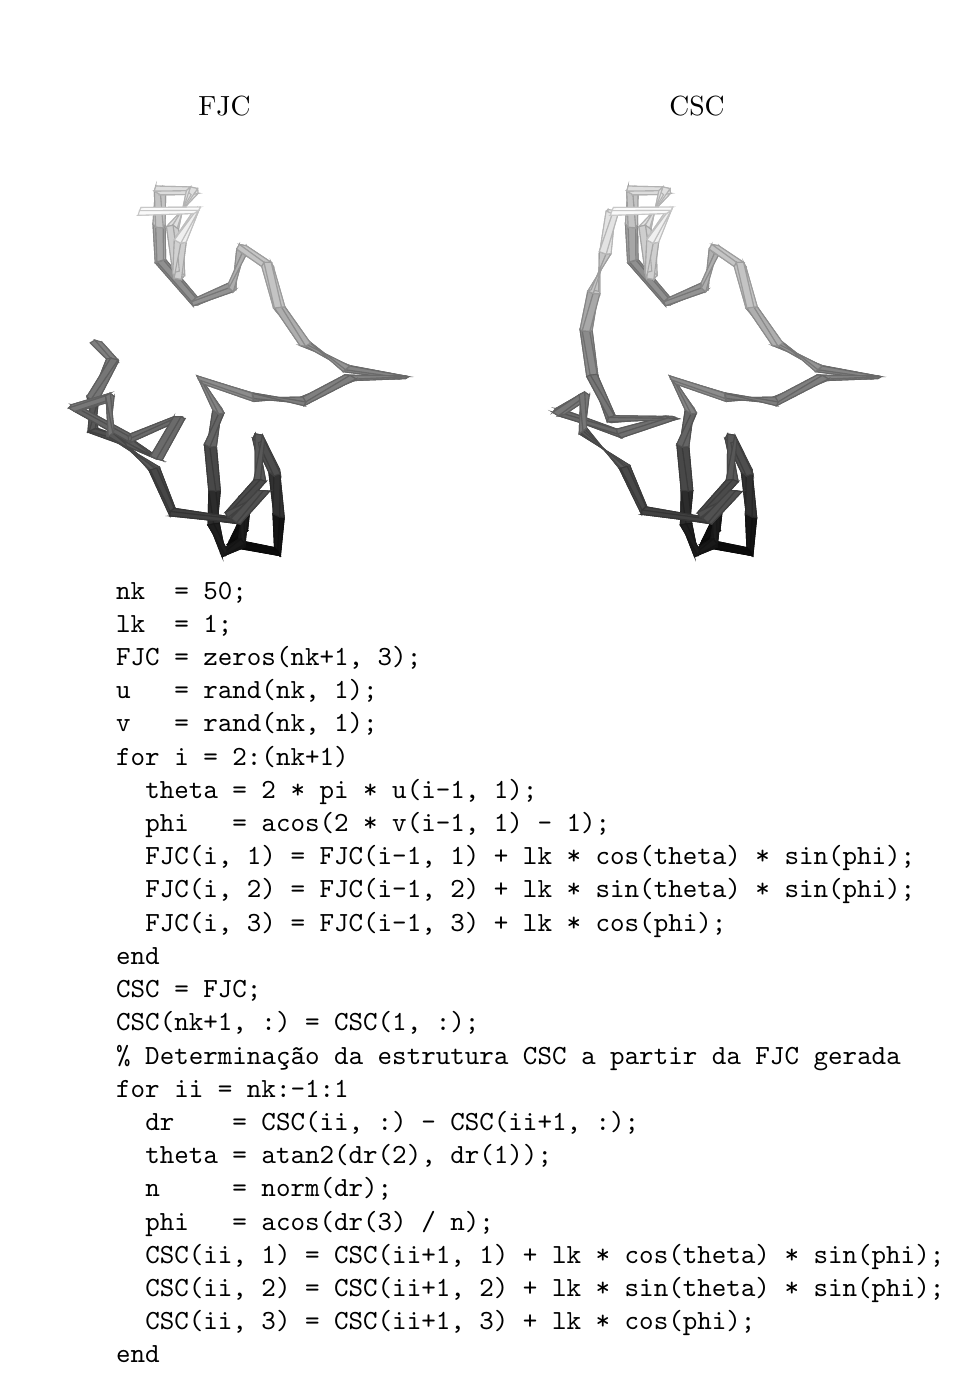
\begin{tikzpicture}

%\draw[help lines] (0,0)grid(14,7);
\useasboundingbox (0,-9)rectangle(11.4,8);
\node at (2.5,7) {FJC};
\node at (8.5,7) {CSC};

\node[right,align=left] at (1,-4)
{\texttt{nk~~=~50;}\\
\texttt{lk~~=~1;}\\
\texttt{FJC~=~zeros(nk+1,~3);}\\
\texttt{u~~~=~rand(nk,~1);}\\
\texttt{v~~~=~rand(nk,~1);}\\
\texttt{for~i~=~2:(nk+1)}\\
\texttt{~~theta~=~2~*~pi~*~u(i-1,~1);}\\
\texttt{~~phi~~~=~acos(2~*~v(i-1, 1)~-~1);}\\
\texttt{~~FJC(i,~1)~=~FJC(i-1,~1)~+~lk~*~cos(theta)~*~sin(phi);}\\
\texttt{~~FJC(i,~2)~=~FJC(i-1,~2)~+~lk~*~sin(theta)~*~sin(phi);}\\
\texttt{~~FJC(i,~3)~=~FJC(i-1,~3)~+~lk~*~cos(phi);}\\
\texttt{end}\\
\texttt{CSC~=~FJC;}\\
\texttt{CSC(nk+1,~:)~=~CSC(1,~:);}\\
\texttt{\% Determinação da estrutura CSC a partir da FJC gerada}\\
\texttt{for~ii~=~nk:-1:1}\\
\texttt{~~dr~~~~=~CSC(ii,~:)~-~CSC(ii+1,~:);}\\
\texttt{~~theta~=~atan2(dr(2),~dr(1));}\\
\texttt{~~n~~~~~=~norm(dr);}\\
\texttt{~~phi~~~=~acos(dr(3)~/~n);}\\
\texttt{~~CSC(ii,~1)~=~CSC(ii+1,~1)~+~lk~*~cos(theta)~*~sin(phi);}\\
\texttt{~~CSC(ii,~2)~=~CSC(ii+1,~2)~+~lk~*~sin(theta)~*~sin(phi);}\\
\texttt{~~CSC(ii,~3)~=~CSC(ii+1,~3)~+~lk~*~cos(phi);}\\
\texttt{end}};




\begin{axis}[%
width=8cm,
height=8cm,
view={-37.5}{30},
scale only axis,
xmin=-4,
xmax=4,
xmajorgrids,
ymin=-4,
ymax=2,
ymajorgrids,
zmin=-8,
zmax=2,
zmajorgrids,
hide axis,
axis x line*=bottom,
axis y line*=left,
axis z line*=left,
at={(-2cm,0cm)},
anchor=south west,
]

\addplot3[%
surf,
colormap/blackwhite,
shader=faceted,
draw=black,
z buffer=sort,
mesh/rows=6]
table[row sep=crcr,header=false] {
-0.00671609406390881 0.012278844200316 -0.0990157768521214\\
0.45527855313052 -0.718832009351433 0.332600332594537\\
0.362581405686629 -0.445324450505241 -0.533761646080799\\
0.356005965714007 -0.524944261547795 -1.46197670889402\\
0.764103473871892 0.0143692555073762 -0.73361635139133\\
1.50551915764327 0.340387517628585 -0.432421462534809\\
1.56409676698225 1.07130018746292 -1.0172903334349\\
1.58492842291217 1.03017227528365 -1.94450347267515\\
1.5895424412439 1.03127389739221 -2.87096773723572\\
1.48599302563838 0.218962374279503 -3.29845081164068\\
1.6684568737146 -0.325398378734288 -2.53434797130208\\
1.89686998619733 -0.396050292965498 -1.72442066898055\\
1.60828298735838 -1.2346019493938 -1.41168425751827\\
1.16695484174602 -1.94028091888288 -1.78199183374815\\
1.46047084197721 -2.26932956390614 -2.60982249850119\\
1.88306199741965 -2.67327887181853 -3.32549344878786\\
2.73277944675734 -2.97962846672309 -3.6789675728018\\
1.83400208553 -2.71057658227331 -3.42521170455354\\
1.04192510193782 -2.56306980098679 -3.82630207105932\\
0.161042598015593 -2.34232382705905 -3.63615069004602\\
-0.591444002177718 -1.98798496125109 -3.12612858327011\\
-0.286244584667919 -2.13220568846827 -4.0315755155991\\
-0.517360552689289 -2.04402395124639 -4.97423401871838\\
-0.821400936617141 -2.47535004195052 -5.77490432517203\\
-0.710447401449985 -2.44353720835221 -6.78152866976386\\
-1.30233080147842 -3.13244016974964 -6.7080377518499\\
-0.527937401831883 -2.68322221550227 -7.13033947348133\\
-0.0907251109109907 -2.38079504278043 -6.4723171900812\\
0.0063003874599662 -2.30625755287955 -7.41587538028378\\
-0.66990256356641 -2.72103562095484 -7.04323003989811\\
0.104381288815308 -2.85824620470814 -7.51537553923111\\
0.0816882350069489 -2.84831637960459 -6.54449401435507\\
0.304512950939243 -2.64894848814904 -5.7005315607294\\
0.108185465389303 -2.501964885242 -4.77349158887928\\
-0.384426697724755 -3.14517376093535 -5.1835476605975\\
-1.28628523786201 -3.39966343948213 -5.53359309980455\\
-1.03833566720097 -3.66447990347261 -4.77642193458517\\
-1.39301228825715 -3.37640199405754 -5.58187091091539\\
-1.94069234076177 -2.65453859674066 -5.64285464945511\\
-1.60519751821597 -1.94440964550032 -5.17572498536818\\
-1.99146075320057 -1.22402986346466 -4.62283707109166\\
-1.92136116830766 -1.26460225210156 -3.63673962293562\\
-2.01036470684725 -0.678429277723869 -4.30299808176534\\
-1.73835423234233 -1.5229421501633 -4.57060979740229\\
-1.11665076859737 -1.82747808272924 -4.06937775677688\\
-1.78414373791246 -2.03005477417655 -4.67481735344807\\
-1.46829729001273 -1.23005197220878 -4.93359060849053\\
-1.39265672053326 -0.38980185273459 -5.32997493271088\\
-1.35976006613141 -0.431277168088693 -4.44292542826602\\
-0.981430990359174 -0.337759929190739 -3.60910610551167\\
-0.560494794505409 0.448400527281186 -3.96795881415894\\
0.0779978458641189 0.0551022154046573 -0.0296661743077177\\
0.557588570218016 -0.701661452545996 0.387894929935043\\
0.451493219596234 -0.519062184194689 -0.555604175470703\\
0.399827187701356 -0.597955495441484 -1.54302435131104\\
0.807174074900364 -0.0657786638118342 -0.808053536106689\\
1.46030989423338 0.398661484382454 -0.340879519070595\\
1.51266151573596 1.15505245626694 -0.952795120341894\\
1.49766598447848 1.10888423343247 -1.94756200099544\\
1.49128964733389 1.07546413712713 -2.91801315479734\\
1.38000211813372 0.207494425891318 -3.34798942081175\\
1.59215930272201 -0.402912597033302 -2.57895611780723\\
2.01093375299905 -0.414095133980907 -1.70243201444617\\
1.69689449547378 -1.27522370676907 -1.34597631606703\\
1.18639830370859 -2.02767612114637 -1.7058098770869\\
1.40971825080315 -2.37239487222739 -2.58489506738072\\
1.89381726648823 -2.61910224124472 -3.42926664860088\\
2.79351836034458 -2.95167475035528 -3.77565797682397\\
1.88633608964006 -2.72222627133218 -3.5298305215567\\
1.0496927441645 -2.48079381058879 -3.90990820271704\\
0.0777881285996758 -2.42526144138219 -3.63303531444076\\
-0.675141984014432 -2.05772148117062 -3.08195703429937\\
-0.402020727113656 -2.12690468336755 -4.01189191080202\\
-0.515223185188279 -1.9267407765213 -4.98196374698468\\
-0.879048261171316 -2.37722836314754 -5.80437604438099\\
-0.822504101768508 -2.43157030128067 -6.74806601653123\\
-1.34726633224268 -3.23278673437762 -6.66643216142268\\
-0.553600654235737 -2.76520063677864 -7.05008614935335\\
-0.0934961473439229 -2.27744575897478 -6.41636268171549\\
-0.0387879742333304 -2.21283593491657 -7.36056623954291\\
-0.777228485332424 -2.75159657518745 -7.00625931220756\\
0.0589453809383789 -2.96628070542903 -7.50622212227955\\
0.11249556869818 -2.96098803252802 -6.55774795455565\\
0.399924095336513 -2.69710085690356 -5.65156501071173\\
0.189268114893791 -2.55569686908736 -4.7074753940944\\
-0.471953046255377 -3.1137767967253 -5.11162388800602\\
-1.31920181422199 -3.30079892606776 -5.47916914275824\\
-0.954404730565471 -3.74552038732502 -4.76201020446846\\
-1.3299450445873 -3.43895836598125 -5.65887015260082\\
-1.88454878114139 -2.64310412024706 -5.74550363178309\\
-1.50538142772803 -1.90423821925015 -5.22308176635287\\
-2.04218654440649 -1.31050818610084 -4.56145259477176\\
-2.02796192573257 -1.25274540972376 -3.58862149830709\\
-2.12448462029263 -0.650578942741922 -4.30754388302713\\
-1.77174467017004 -1.53124758963707 -4.68301868694988\\
-1.01904599264726 -1.88281523925606 -4.10446004478317\\
-1.71742619588163 -2.1201611160842 -4.71016246408428\\
-1.39701122202518 -1.27233926072027 -5.01695572022033\\
-1.29759682694289 -0.353907154007744 -5.38909216663127\\
-1.39614998638501 -0.320535724726604 -4.42770154773185\\
-1.06174499329717 -0.313904972105368 -3.52664240399984\\
-0.611591938726288 0.485758778525975 -3.8688977066096\\
0.0549214138572097 0.0217761977751802 0.0806810728137729\\
0.563795856013529 -0.77776862124203 0.477275177129976\\
0.406382703576596 -0.626215550235059 -0.573006979933247\\
0.327898651975503 -0.596413845244197 -1.63599514874499\\
0.755791195307873 -0.049627341779768 -0.91254561520315\\
1.52844053230624 0.37788833274795 -0.247357583464793\\
1.59505736038907 1.20449526142227 -0.885075153457864\\
1.54559350503924 1.21600375842668 -1.95449166551923\\
1.52193247861349 1.1436296938451 -3.0087552832769\\
1.3953158059559 0.19333199012112 -3.46368115124587\\
1.64108685560027 -0.451320986153163 -2.6742576526567\\
2.04163936643913 -0.346025614478536 -1.61163903051852\\
1.67166460998464 -1.25313388009625 -1.23330354851306\\
1.08482340941027 -2.05218354048831 -1.65194349278292\\
1.29971917505696 -2.36967146909883 -2.62627678463464\\
2.00413380943288 -2.5795029868146 -3.43831206256706\\
2.8971936082932 -3.00686592408387 -3.77065423644749\\
1.92929112412023 -2.83141909225538 -3.53700359510596\\
1.01741146253783 -2.52949789879985 -4.01191551010514\\
0.043456346075823 -2.43809344622633 -3.5213378280191\\
-0.718076746791422 -2.00625515281549 -2.98537813751842\\
-0.425849915396308 -2.0226003022982 -3.96318435504289\\
-0.403040780104768 -1.89302592978843 -4.99186714094633\\
-0.804942500773882 -2.30804179310075 -5.86388415234604\\
-0.874830284675388 -2.35697800213535 -6.8223466977553\\
-1.42192870305356 -3.27519965358407 -6.74672123154923\\
-0.569951942891345 -2.86716582593714 -7.10625905805205\\
0.0153899049169412 -2.25333255044652 -6.37918687089692\\
0.0262203461012755 -2.1190420688659 -7.38878483431733\\
-0.847933595797418 -2.75648825261694 -7.10004907155558\\
0.0713524148285777 -3.01983208456449 -7.61013542948916\\
0.213977481042452 -2.96417236797524 -6.61700115351748\\
0.466749177535142 -2.61020220534395 -5.60910688005612\\
0.218773151510569 -2.48304483435998 -4.61989232052014\\
-0.533895783157615 -3.0290679171219 -5.16460655662413\\
-1.39121477681631 -3.24198155593321 -5.55110182171118\\
-0.990127894290339 -3.82040312701868 -4.67872700699166\\
-1.37208848228436 -3.54869856890985 -5.65969394430058\\
-1.96209237879742 -2.66257182117851 -5.8316875003172\\
-1.53357711522254 -1.8282154405246 -5.30820050949479\\
-1.97031955246509 -1.33923767498581 -4.47296862983911\\
-2.0138210919325 -1.21986983919996 -3.47664429618686\\
-2.13410826750389 -0.534313374794846 -4.2930744933787\\
-1.72317086236074 -1.44193320036932 -4.74203720249487\\
-0.98748435626103 -1.95800249392946 -4.01978183060855\\
-1.76677684160025 -2.21943432141951 -4.67105997590119\\
-1.45981504669817 -1.2848509252648 -5.11553968427773\\
-1.33384374486517 -0.289463605817522 -5.4804860950417\\
-1.50963881670833 -0.323461024930023 -4.39718289567994\\
-1.05354262561383 -0.396172216661287 -3.44306919208319\\
-0.554953454795875 0.43696686800097 -3.77817234236185\\
-0.0440545453901638 -0.0416437850338561 0.0795298195554345\\
0.465322152525545 -0.841975995089138 0.477220610478806\\
0.289591057516809 -0.618702238767518 -0.561919975200763\\
0.239623150148565 -0.522449819129822 -1.61240661910333\\
0.680964228251398 0.0405026435185043 -0.902688086924546\\
1.61575684572037 0.306775852230503 -0.281099792030943\\
1.69741604416273 1.15130032670338 -0.907717125299524\\
1.662476780176 1.20349530758303 -1.95571590540527\\
1.63912358376583 1.14156808502394 -3.01779158532715\\
1.51077109302778 0.196047071839836 -3.48564396370037\\
1.74762331725798 -0.403724797670855 -2.68854909386856\\
1.94655271238879 -0.285911496812787 -1.5775145350456\\
1.56746017510468 -1.1988598590316 -1.22937589000943\\
1.00260321036766 -1.9799347563547 -1.69483419309324\\
1.28248859868879 -2.26492300507906 -2.67677952353087\\
2.06155791342549 -2.60920593222143 -3.34012923602746\\
2.90052952173027 -3.06892966169494 -3.67087135080178\\
1.90350479130683 -2.88725427785453 -3.43681798136004\\
0.989692891065467 -2.64187467110335 -3.99135336151413\\
0.10549260699763 -2.36308644704067 -3.45542036055785\\
-0.660913907649801 -1.90471069269631 -2.96986064568256\\
-0.32480102123357 -1.96343765472252 -3.95276503487189\\
-0.33584560832446 -1.98947218330712 -4.99025804675231\\
-0.701495297531938 -2.36340382004979 -5.87119046646568\\
-0.79511294389486 -2.32284433303608 -6.9017173366919\\
-1.42313705513109 -3.20106571458778 -6.83794819623979\\
-0.554394342636519 -2.84820535723004 -7.22122914900278\\
0.0854562225478848 -2.34177905180389 -6.41216546461741\\
0.111486059312899 -2.15449588967331 -7.46153402574355\\
-0.784305835477087 -2.72895052129775 -7.19498505831988\\
0.124456291349221 -2.94489415629375 -7.68351080217966\\
0.245889418423318 -2.85346874258978 -6.64036770421747\\
0.41263820523763 -2.50834351634906 -5.63183286222983\\
0.155925617474559 -2.38441142370126 -4.63177919899694\\
-0.484652151388769 -3.00811191458811 -5.26927541923627\\
-1.40280465897019 -3.30449493547555 -5.64998261925224\\
-1.09613696029348 -3.78564272146766 -4.64166689037594\\
-1.46120180285375 -3.55396537232833 -5.58320383388525\\
-2.06616051737918 -2.68603799853057 -5.78230307802525\\
-1.65081909891825 -1.82140220560317 -5.31345000485147\\
-1.87517751757016 -1.27051515295996 -4.47966700837127\\
-1.89848081858989 -1.21140846159451 -3.45555670393997\\
-2.02593609513079 -0.490307637064189 -4.27958611751771\\
-1.65976016034387 -1.37842843264365 -4.66610376151966\\
-1.06558296818389 -1.9491336163116 -3.93236552813571\\
-1.86399476005195 -2.19068219458123 -4.61154819852313\\
-1.56991601295711 -1.25029627069767 -5.0931028130811\\
-1.45130546571893 -0.285530001407168 -5.47785341524434\\
-1.54338885093801 -0.436010403245122 -4.39354521195521\\
-0.968159280659318 -0.470871127043017 -3.47388180808153\\
-0.468851802434737 0.369453557675684 -3.82116209116438\\
-0.082148620267256 -0.0475134723462975 -0.0315289412093683\\
0.398254770976379 -0.805551165758988 0.387806639238798\\
0.26252036666945 -0.506905390872143 -0.537665024980113\\
0.256994425371417 -0.47827918724364 -1.5048573086062\\
0.686101498927919 0.0800547158062987 -0.792103720306844\\
1.60159065710978 0.283599073880909 -0.395475559386113\\
1.67828134512545 1.06898124386245 -0.989430600354017\\
1.68678709636615 1.08864513482084 -1.94954286274145\\
1.68090883864953 1.07212838398299 -2.93263419864726\\
1.56681269679689 0.211887520394433 -3.38352599785167\\
1.76453891872534 -0.32590034633398 -2.60208015543624\\
1.8570803148691 -0.316828448394015 -1.64721742092203\\
1.52828817805953 -1.18740649598032 -1.33962123111195\\
1.05336322709587 -1.91077513277233 -1.77520848799029\\
1.38183859259371 -2.20290829717406 -2.66661021543978\\
1.98673141852177 -2.66716261647896 -3.27040349814826\\
2.79891598166929 -3.05209598727886 -3.61420587635366\\
1.84461292670277 -2.81256949939976 -3.36772679333204\\
1.00484315340262 -2.66262324772186 -3.87663794741505\\
0.178164907306116 -2.30389756730566 -3.52637861163613\\
-0.582650567389847 -1.89341909332854 -3.0568492050888\\
-0.238520181832755 -2.03117750872569 -3.99503309662568\\
-0.406499113367852 -2.08279409280212 -4.97936017788766\\
-0.711667170284731 -2.46680600443717 -5.81619790895905\\
-0.693518734892857 -2.37634086451731 -6.87649040803945\\
-1.34922148697448 -3.11283550136171 -6.81404049098248\\
-0.528427928240043 -2.73452195396792 -7.2361116642013\\
0.0198735360494899 -2.42055520435702 -6.46972316725642\\
0.0991748478180781 -2.27020142201401 -7.47827690392462\\
-0.674276606506096 -2.70703958993995 -7.15986896554771\\
0.144869258083158 -2.84502859044047 -7.62494596922998\\
0.16413016802728 -2.7818658039765 -6.59555582778808\\
0.312370702994835 -2.53229003606032 -5.68833642229652\\
0.0875786687144113 -2.39610465821523 -4.72670876749001\\
-0.3922751763239 -3.07986927235731 -5.28098166527626\\
-1.33795463747257 -3.40194769891888 -5.63916163401437\\
-1.12593100247418 -3.68927686968074 -4.70204567615718\\
-1.47413342611894 -3.44748023292441 -5.53510655414558\\
-2.05293456651261 -2.68107319278873 -5.66559795799994\\
-1.69508294225616 -1.89321417357394 -5.23157562826377\\
-1.88824349818767 -1.1993128096704 -4.57229079890631\\
-1.84133744319252 -1.2390546131665 -3.55450105731072\\
-1.94945836875605 -0.579376163393706 -4.28571923243102\\
-1.66914399905625 -1.42849471700926 -4.56015579856924\\
-1.14541220121263 -1.8684650938283 -3.96301749621127\\
-1.87472809225199 -2.07363919761101 -4.61387038555567\\
-1.57515832762636 -1.21642865516114 -4.98065210002298\\
-1.48765388366134 -0.347542448373496 -5.38483240123764\\
-1.45075868889011 -0.502644444253104 -4.42181565182491\\
-0.923591839087602 -0.434770348025589 -3.57649826396745\\
-0.472276538718438 0.376519947726643 -3.9384565813399\\
-0.00671609406390883 0.012278844200316 -0.0990157768521214\\
0.45527855313052 -0.718832009351433 0.332600332594537\\
0.362581405686629 -0.445324450505241 -0.533761646080799\\
0.356005965714007 -0.524944261547795 -1.46197670889402\\
0.764103473871892 0.0143692555073762 -0.73361635139133\\
1.50551915764327 0.340387517628585 -0.432421462534809\\
1.56409676698225 1.07130018746292 -1.0172903334349\\
1.58492842291217 1.03017227528365 -1.94450347267515\\
1.5895424412439 1.03127389739221 -2.87096773723572\\
1.48599302563838 0.218962374279503 -3.29845081164068\\
1.6684568737146 -0.325398378734288 -2.53434797130208\\
1.89686998619733 -0.396050292965498 -1.72442066898055\\
1.60828298735838 -1.2346019493938 -1.41168425751827\\
1.16695484174602 -1.94028091888288 -1.78199183374815\\
1.46047084197721 -2.26932956390614 -2.60982249850119\\
1.88306199741965 -2.67327887181853 -3.32549344878786\\
2.73277944675734 -2.97962846672309 -3.6789675728018\\
1.83400208553 -2.71057658227331 -3.42521170455354\\
1.04192510193782 -2.56306980098679 -3.82630207105932\\
0.161042598015593 -2.34232382705905 -3.63615069004602\\
-0.591444002177718 -1.98798496125109 -3.12612858327011\\
-0.286244584667919 -2.13220568846827 -4.0315755155991\\
-0.517360552689289 -2.04402395124639 -4.97423401871838\\
-0.821400936617141 -2.47535004195052 -5.77490432517203\\
-0.710447401449985 -2.44353720835221 -6.78152866976386\\
-1.30233080147842 -3.13244016974964 -6.7080377518499\\
-0.527937401831883 -2.68322221550227 -7.13033947348133\\
-0.0907251109109906 -2.38079504278043 -6.4723171900812\\
0.00630038745996622 -2.30625755287955 -7.41587538028378\\
-0.66990256356641 -2.72103562095484 -7.04323003989811\\
0.104381288815308 -2.85824620470814 -7.51537553923111\\
0.0816882350069489 -2.84831637960459 -6.54449401435507\\
0.304512950939243 -2.64894848814904 -5.7005315607294\\
0.108185465389303 -2.501964885242 -4.77349158887928\\
-0.384426697724755 -3.14517376093535 -5.1835476605975\\
-1.28628523786201 -3.39966343948213 -5.53359309980455\\
-1.03833566720097 -3.66447990347261 -4.77642193458517\\
-1.39301228825715 -3.37640199405754 -5.58187091091538\\
-1.94069234076177 -2.65453859674066 -5.64285464945511\\
-1.60519751821597 -1.94440964550032 -5.17572498536818\\
-1.99146075320057 -1.22402986346466 -4.62283707109166\\
-1.92136116830766 -1.26460225210156 -3.63673962293562\\
-2.01036470684725 -0.678429277723869 -4.30299808176534\\
-1.73835423234233 -1.5229421501633 -4.57060979740229\\
-1.11665076859737 -1.82747808272924 -4.06937775677688\\
-1.78414373791246 -2.03005477417655 -4.67481735344807\\
-1.46829729001273 -1.23005197220878 -4.93359060849053\\
-1.39265672053326 -0.38980185273459 -5.32997493271088\\
-1.35976006613141 -0.431277168088693 -4.44292542826602\\
-0.981430990359174 -0.337759929190739 -3.60910610551167\\
-0.560494794505409 0.448400527281186 -3.96795881415894\\
};
\end{axis}

\begin{axis}[%
width=8cm,
height=8cm,
view={-37.5}{30},
scale only axis,
xmin=-4,
xmax=4,
xmajorgrids,
ymin=-4,
ymax=2,
ymajorgrids,
zmin=-8,
zmax=2,
zmajorgrids,
hide axis,
axis x line*=bottom,
axis y line*=left,
axis z line*=left,
at={(4cm,0cm)},
anchor=south west,
]

\addplot3[%
surf,
colormap/blackwhite,
shader=faceted,
draw=black,
z buffer=sort,
mesh/rows=6]
table[row sep=crcr,header=false] {
-0.00671609406825905 0.0122788442070508 -0.0990157768553682\\
0.455278553128405 -0.718832009348545 0.332600332582467\\
0.362581405685455 -0.445324450505175 -0.533761646093998\\
0.356005965700612 -0.524944261581113 -1.46197670889919\\
0.764103473791928 0.0143692554818785 -0.733616351382459\\
1.50551915758213 0.340387516915873 -0.432421461938537\\
1.5640967670091 1.07130018756311 -1.01729033191695\\
1.58492842256752 1.03017227534332 -1.94450347170761\\
1.58954244132538 1.03127389953095 -2.87096773637457\\
1.48599302245521 0.218962389535666 -3.29845082992028\\
1.66845687808505 -0.325398374870305 -2.53434800006641\\
1.89687001997044 -0.396050178709472 -1.7244207034363\\
1.60828306967965 -1.23460181156165 -1.41168417596044\\
1.16695471676055 -1.94028079301864 -1.78199147528604\\
1.46047058030477 -2.26932941498362 -2.60982219628093\\
1.88306149188697 -2.67327862680308 -3.32549338858341\\
2.7327789669741 -2.97962835335045 -3.67896743335608\\
1.83400150295535 -2.71057650099264 -3.42521185067949\\
1.04192418015893 -2.56306960448878 -3.82630168838076\\
0.161041744670919 -2.34232338751053 -3.63615014322898\\
-0.591444450202441 -1.98798481032269 -3.12612720599086\\
-0.286244452475101 -2.13220581468717 -4.03157391776766\\
-0.517359105836068 -2.04402416843821 -4.97423167761358\\
-0.821402736724217 -2.47534851648754 -5.77490101276369\\
-0.710464420646205 -2.44356375171364 -6.78153116268928\\
-1.30235511997619 -3.13245179693983 -6.70803050184565\\
-0.527976841792506 -2.6832695479361 -7.13039614637419\\
-0.0907068936705208 -2.38078765968689 -6.47247443765824\\
0.00654814999823315 -2.306060407152 -7.41606602271062\\
-0.669479138209456 -2.72113931036446 -7.0434737274209\\
0.104353479288329 -2.85834324299114 -7.51644886939204\\
0.0814156605264879 -2.84870748611057 -6.54557698591455\\
0.304783912662045 -2.64902825970891 -5.70185323316124\\
0.106407159846958 -2.50361532903349 -4.77514656578394\\
-0.387733391514647 -3.1464159219121 -5.18532776040962\\
-1.29340133913901 -3.39780138525656 -5.53406030260022\\
-1.04042020563525 -3.6616882780789 -4.78166979667606\\
-1.39796930790156 -3.36572856727938 -5.58326605493825\\
-1.92931709107408 -2.62968221094515 -5.62448740083495\\
-1.62051525704666 -1.91756839125682 -5.14040899855129\\
-1.95798535109784 -1.22073120385456 -4.5585892311837\\
-1.91060517619288 -1.31227232805913 -3.5625566814709\\
-1.92705909643256 -0.84779900443917 -4.32369285504915\\
-1.51503441348891 -1.58004137831629 -4.37695284947555\\
-0.891823698442124 -2.05719274136445 -3.91149286015859\\
-1.36966411238193 -1.43832128493224 -4.24923503911533\\
-1.05457286849413 -0.703167023508618 -3.67310634997153\\
-0.82532918096562 -0.317997118312758 -2.83308587611077\\
-0.562583621813539 -0.281963915912617 -1.89251340840561\\
-0.274339300665578 -0.00638013620882602 -0.96444960280492\\
-0.0878183129193184 0.0426485316134734 0.0216574852468896\\
0.0779978458600623 0.0551022154110145 -0.02966617431109\\
0.557588570216101 -0.701661452542984 0.387894929922565\\
0.45149321959555 -0.519062184194006 -0.555604175483992\\
0.399827187689275 -0.597955495459225 -1.54302435132954\\
0.807174074814333 -0.0657786638710251 -0.808053536065051\\
1.46030989416101 0.398661483600943 -0.340879518436077\\
1.51266151576624 1.15505245629853 -0.952795118732141\\
1.49766598441982 1.10888423382605 -1.94756199959443\\
1.49128964763621 1.07546414022177 -2.91801315349952\\
1.38000211407956 0.207494440369541 -3.34798943704772\\
1.59215929599541 -0.402912587651002 -2.57895613718021\\
2.01093378837583 -0.414095024456629 -1.70243206110386\\
1.69689458652895 -1.27522356945475 -1.34597624660755\\
1.18639819584325 -2.02767599223905 -1.70580951950327\\
1.40971799581058 -2.37239472409906 -2.58489475484382\\
1.89381688850941 -2.61910185782414 -3.42926650291944\\
2.79351793838628 -2.95167449192236 -3.77565775911595\\
1.88633551709708 -2.72222597129581 -3.52983068702348\\
1.04969180312798 -2.48079360372347 -3.90990781162528\\
0.0777872575279732 -2.42526098322564 -3.633034745973\\
-0.67514243416959 -2.05772134464917 -3.08195568380216\\
-0.40202060268336 -2.12690473832113 -4.01189037782138\\
-0.515223254848019 -1.9267409746676 -4.98196153608719\\
-0.879047735974607 -2.3772258179142 -5.80437388501272\\
-0.822519324661075 -2.43159293870325 -6.74806389159363\\
-1.34728132784645 -3.23280174149713 -6.66642299547664\\
-0.553626735813066 -2.76526006811543 -7.05015091193651\\
-0.0934927916988086 -2.2774275838306 -6.41654060528766\\
-0.0385383275498328 -2.21265492698666 -7.36072809783184\\
-0.776788567043536 -2.75176581455606 -7.00650936841379\\
0.0589029123010766 -2.96637577661542 -7.50734514752912\\
0.112301044558886 -2.96135645933594 -6.55884205270452\\
0.400122477192943 -2.69729933291627 -5.65286219605139\\
0.187330103656585 -2.5575649088502 -4.70911187705684\\
-0.475093311045244 -3.11515660004524 -5.11314217065285\\
-1.32607041028925 -3.29641811739296 -5.48432274234663\\
-0.959953301510822 -3.74691733788369 -4.77268398464138\\
-1.33748037891076 -3.4294294949811 -5.66138737976053\\
-1.87195704892155 -2.61539467390506 -5.72610113987692\\
-1.52171985796871 -1.87449263579085 -5.18735160738981\\
-2.04539340103216 -1.28006201435989 -4.50702036611997\\
-2.01989061392464 -1.28364202307645 -3.53005039209672\\
-2.03644806695682 -0.813021323984072 -4.34907446615458\\
-1.58060684381927 -1.66906608887533 -4.4168842582029\\
-0.944680889304706 -2.15271410553476 -3.86788728168907\\
-1.45683555341924 -1.42504987340495 -4.32698251248941\\
-0.992552553843685 -0.659396059421309 -3.76286849893215\\
-0.726983855857177 -0.275172621172881 -2.88118909415834\\
-0.495803877096984 -0.190558554810348 -1.92421807320208\\
-0.362606283308925 -0.0763251198089552 -0.93074056608303\\
-0.0637662708039324 -0.0723184472450925 0.0265312060754563\\
0.0549214138535964 0.0217761977809737 0.0806810728103231\\
0.563795856012117 -0.777768621239091 0.4772751771174\\
0.406382703576651 -0.626215550234717 -0.573006979946353\\
0.327898651971058 -0.596413845235287 -1.63599514876896\\
0.755791195312229 -0.0496273418002787 -0.912545615199981\\
1.52844053223165 0.377888331909349 -0.247357582841344\\
1.59505736041208 1.20449526134336 -0.885075151758587\\
1.54559350537195 1.21600375869171 -1.95449166339852\\
1.52193247926031 1.14362969773276 -3.00875528126703\\
1.3953157998944 0.193332002225114 -3.4636811674569\\
1.64108683646225 -0.451320985409733 -2.67425767401357\\
2.0416394174447 -0.346025496678627 -1.61163908866619\\
1.67166472298389 -1.25313373021423 -1.23330347660376\\
1.08482331437139 -2.05218340719866 -1.65194310901884\\
1.29971890989095 -2.36967132070855 -2.62627644503791\\
2.00413348687814 -2.57950273027975 -3.43831179642363\\
2.89719315841045 -3.00686572271068 -3.77065406952605\\
1.92929053866069 -2.83141878216089 -3.53700399102888\\
1.017410483224 -2.52949767514532 -4.01191511491623\\
0.0434555096380887 -2.43809298882196 -3.52133724899253\\
-0.718077201856609 -2.0062550476211 -2.98537677250999\\
-0.425849747348319 -2.02260036187384 -3.9631827908253\\
-0.40304134899108 -1.89302474778813 -4.9918658864353\\
-0.804940390038769 -2.30804178314737 -5.86388296603596\\
-0.874844992877114 -2.3569959123902 -6.82234018810534\\
-1.42195054382088 -3.27521575727844 -6.7467051202839\\
-0.569999422789559 -2.86721419252873 -7.10633766970724\\
0.0153851064964364 -2.2533029201114 -6.37934834806224\\
0.0265207120568996 -2.11886822493674 -7.38885345999042\\
-0.847504192609153 -2.7566214445508 -7.10029307313225\\
0.0712571055881424 -3.01986309373657 -7.61129773733769\\
0.213780988911184 -2.96446493862673 -6.61810264975901\\
0.46701716113306 -2.61048730120472 -5.61033652706001\\
0.216823406292475 -2.48509324224152 -4.62137555190534\\
-0.536740636108127 -3.02986110277188 -5.16552485452818\\
-1.39130237487352 -3.23715087848285 -5.56211634941656\\
-0.99509061741992 -3.8213482618055 -4.68874908899391\\
-1.38209159420825 -3.53819174785159 -5.66190885144428\\
-1.94854237041079 -2.63210357730304 -5.81370913718383\\
-1.55177696801592 -1.79645678182714 -5.26997506498065\\
-2.00443774242552 -1.32488125431166 -4.40635493078717\\
-2.0170236898567 -1.25206306529342 -3.4168505233502\\
-2.04158675639765 -0.69638021665849 -4.3353592896995\\
-1.53547085209285 -1.70421730954413 -4.51958184361204\\
-0.869398475911585 -2.24266201261473 -3.87573536159054\\
-1.55783381666197 -1.41722868006201 -4.26733488161319\\
-1.06334781013838 -0.589153087918632 -3.82510688542428\\
-0.749757188648715 -0.166485891769634 -2.91976668192238\\
-0.563033934612226 -0.0941378210383778 -1.92253831790048\\
-0.323918674054621 -0.187310005656645 -0.933039286610329\\
0.0484085902266581 -0.0873437900245568 -0.00526029812972989\\
-0.0440545453937967 -0.0416437850280335 0.0795298195520622\\
0.465322152524243 -0.841975995086368 0.477220610466579\\
0.289591057516829 -0.618702238768004 -0.561919975213667\\
0.239623150147527 -0.522449819120017 -1.61240661911735\\
0.680964228317685 0.0405026435555927 -0.902688086977919\\
1.61575684565566 0.306775851425416 -0.281099791452579\\
1.69741604417783 1.15130032662477 -0.90771712363672\\
1.66247678046459 1.20349530743471 -1.95571590327324\\
1.63912358440471 1.14156808844581 -3.01779158331388\\
1.51077108659667 0.196047083254413 -3.48564398193962\\
1.74762330154633 -0.403724807784856 -2.68854912584288\\
1.94655277144981 -0.28591136916651 -1.57751458809253\\
1.56746029293222 -1.19885970086448 -1.2293758044877\\
1.00260310613585 -1.97993462339969 -1.69483379227027\\
1.28248832055538 -2.26492285573269 -2.67677917752688\\
2.06155749757084 -2.6092058925114 -3.34012898091142\\
2.90052899676432 -3.06892964064689 -3.67087129353046\\
1.90350418783277 -2.88725418029947 -3.43681850037186\\
0.989691907352585 -2.64187444743985 -3.99135297220624\\
0.105491809691894 -2.3630860087092 -3.45541979665629\\
-0.660914363619119 -1.90471059245616 -2.96985924492367\\
-0.324800818465842 -1.9634377884201 -3.95276338649801\\
-0.3358449692368 -1.98947016737483 -4.99025725311331\\
-0.701494532183985 -2.36340639675597 -5.87118872849855\\
-0.795129130303807 -2.32286322767945 -6.90171273500369\\
-1.42317244933612 -3.20107911607337 -6.83792970847285\\
-0.554468405807634 -2.84823478653006 -7.22130823016489\\
0.0854612462330364 -2.34175313382205 -6.41229610134917\\
0.111815887357352 -2.15431033554248 -7.46157381462911\\
-0.783899423910335 -2.72899588473273 -7.19521894924624\\
0.124342983930388 -2.94488754006021 -7.68464769292088\\
0.245613659664955 -2.8537371112564 -6.64146264614232\\
0.413021784943835 -2.50856344176718 -5.63304525533885\\
0.154128325952314 -2.3863537092393 -4.6331862096408\\
-0.487480858781906 -3.00840490823648 -5.27008472334185\\
-1.39894887498928 -3.30190497828065 -5.65993300294682\\
-1.09727357704961 -3.78212004279844 -4.64586028267628\\
-1.47015177053234 -3.54170958911685 -5.58410981384674\\
-2.05323474428301 -2.65671778455782 -5.76624011816384\\
-1.66914868270663 -1.79130372720242 -5.27409656120131\\
-1.89171770344066 -1.29325025744646 -4.39570913532292\\
-1.90596639560779 -1.2611765010369 -3.37939544631701\\
-1.93537367060545 -0.659069728300954 -4.30150123338314\\
-1.44200284475963 -1.63691724810445 -4.54312103323008\\
-0.770014194816934 -2.20273151223678 -3.9241913201856\\
-1.53308273511338 -1.42566632827078 -4.15272314500921\\
-1.16912199942121 -0.589511508146496 -3.77381017472075\\
-0.862177207459441 -0.142138296012242 -2.89550572431697\\
-0.671364139938811 -0.125951891449364 -1.88979550723485\\
-0.211741433948638 -0.185957453747915 -0.968169010748727\\
0.0936844249114731 0.0183370163036824 -0.0297822491105869\\
-0.0821486202713443 -0.0475134723398931 -0.0315289412126151\\
0.398254770974643 -0.80555116575625 0.387806639226883\\
0.262520366668711 -0.5069053908728 -0.537665024993075\\
0.256994425364848 -0.478279187259934 -1.50485730860861\\
0.686101498942092 0.0800547158403049 -0.792103720356694\\
1.60159065705339 0.283599073153626 -0.395475558824546\\
1.67828134514292 1.06898124389452 -0.98943059880328\\
1.68678709623611 1.0886451345456 -1.94954286132211\\
1.68090883893902 1.07212838632397 -2.93263419734394\\
1.56681269214469 0.211887533757158 -3.38352601736937\\
1.76453891754272 -0.325900354519374 -2.60208019198862\\
1.85708036327988 -0.316828322937978 -1.64721745932655\\
1.52828827692704 -1.18740634526044 -1.3396211396271\\
1.05336310435604 -1.91077500440647 -1.7752081028048\\
1.38183831661944 -2.20290814749875 -2.66660989253572\\
1.98673088958054 -2.66716258388831 -3.27040337030951\\
2.79891543822383 -3.05209602061814 -3.61420583606328\\
1.84461232501166 -2.81256954325941 -3.36772715796084\\
1.00484220524828 -2.66262304084201 -3.87663756583899\\
0.178164099551317 -2.30389714000971 -3.52637806764117\\
-0.582651019007918 -1.89341896482322 -3.05684779674613\\
-0.238520001224742 -2.03117768361106 -3.9950314274773\\
-0.406497228484649 -2.08279294161813 -4.97935871269677\\
-0.711668821970175 -2.46680764450691 -5.81619485699094\\
-0.693536349574947 -2.37636509471397 -6.87649137024881\\
-1.34925841250116 -3.11284613621557 -6.81402747977608\\
-0.52849702245646 -2.73455074412329 -7.23617718646261\\
0.0198927841953974 -2.42054303592663 -6.46985118995887\\
0.0994721651626793 -2.27000146657978 -7.47839210331118\\
-0.673873889442273 -2.70706671981219 -7.1601026623781\\
0.144797667781471 -2.84506278244172 -7.62602786873602\\
0.163807387791172 -2.78219507115031 -6.5966393208298\\
0.312756123283441 -2.53238306408177 -5.68960569024784\\
0.0858873327387993 -2.39780098841931 -4.72822192270231\\
-0.395389317053166 -3.08043974801773 -5.28232359225259\\
-1.33844270737154 -3.40119245177669 -5.64259341242436\\
-1.12528880326273 -3.68344474621215 -4.70328843828254\\
-1.47996473725845 -3.43512148171531 -5.53550589263567\\
-2.04135286820971 -2.65522129784943 -5.64929465368996\\
-1.71163128165614 -1.86615481826216 -5.19402032835934\\
-1.86300854674145 -1.22888198633395 -4.48979510722154\\
-1.84019613713131 -1.29838787186368 -3.46944680440577\\
-1.86459168409503 -0.752651685684722 -4.29429098024169\\
-1.4293724310934 -1.56017230202098 -4.45497146707252\\
-0.783873744546086 -2.08810519873543 -3.94629066965333\\
-1.41678746221529 -1.43870227499185 -4.14153682715451\\
-1.16369878723577 -0.659975995532249 -3.67986867750277\\
-0.908883267308834 -0.235777383693078 -2.84193404015316\\
-0.671085831323653 -0.242034802055807 -1.87123909265787\\
-0.181099696053287 -0.0741366448490817 -0.987581653754365\\
0.00949156858511964 0.0986766893524935 -0.0131461440820291\\
-0.00671609406825907 0.0122788442070508 -0.0990157768553682\\
0.455278553128405 -0.718832009348545 0.332600332582467\\
0.362581405685455 -0.445324450505175 -0.533761646093998\\
0.356005965700612 -0.524944261581113 -1.46197670889919\\
0.764103473791928 0.0143692554818785 -0.733616351382459\\
1.50551915758213 0.340387516915872 -0.432421461938537\\
1.5640967670091 1.07130018756311 -1.01729033191695\\
1.58492842256752 1.03017227534332 -1.94450347170761\\
1.58954244132538 1.03127389953095 -2.87096773637457\\
1.48599302245521 0.218962389535666 -3.29845082992028\\
1.66845687808505 -0.325398374870305 -2.53434800006641\\
1.89687001997044 -0.396050178709472 -1.7244207034363\\
1.60828306967965 -1.23460181156165 -1.41168417596044\\
1.16695471676055 -1.94028079301864 -1.78199147528604\\
1.46047058030477 -2.26932941498362 -2.60982219628093\\
1.88306149188697 -2.67327862680308 -3.32549338858341\\
2.7327789669741 -2.97962835335045 -3.67896743335608\\
1.83400150295535 -2.71057650099264 -3.42521185067949\\
1.04192418015893 -2.56306960448878 -3.82630168838076\\
0.161041744670919 -2.34232338751053 -3.63615014322898\\
-0.591444450202441 -1.98798481032269 -3.12612720599086\\
-0.286244452475101 -2.13220581468717 -4.03157391776766\\
-0.517359105836068 -2.04402416843821 -4.97423167761358\\
-0.821402736724217 -2.47534851648754 -5.77490101276369\\
-0.710464420646205 -2.44356375171364 -6.78153116268928\\
-1.30235511997619 -3.13245179693983 -6.70803050184565\\
-0.527976841792506 -2.6832695479361 -7.13039614637419\\
-0.0907068936705208 -2.38078765968689 -6.47247443765824\\
0.00654814999823316 -2.306060407152 -7.41606602271062\\
-0.669479138209456 -2.72113931036446 -7.0434737274209\\
0.104353479288329 -2.85834324299114 -7.51644886939205\\
0.0814156605264879 -2.84870748611057 -6.54557698591455\\
0.304783912662045 -2.64902825970891 -5.70185323316124\\
0.106407159846958 -2.50361532903349 -4.77514656578394\\
-0.387733391514647 -3.1464159219121 -5.18532776040962\\
-1.29340133913901 -3.39780138525656 -5.53406030260022\\
-1.04042020563525 -3.6616882780789 -4.78166979667606\\
-1.39796930790156 -3.36572856727938 -5.58326605493825\\
-1.92931709107408 -2.62968221094515 -5.62448740083495\\
-1.62051525704666 -1.91756839125682 -5.14040899855129\\
-1.95798535109784 -1.22073120385456 -4.5585892311837\\
-1.91060517619288 -1.31227232805913 -3.5625566814709\\
-1.92705909643256 -0.84779900443917 -4.32369285504915\\
-1.51503441348891 -1.58004137831629 -4.37695284947555\\
-0.891823698442124 -2.05719274136445 -3.91149286015859\\
-1.36966411238193 -1.43832128493224 -4.24923503911533\\
-1.05457286849413 -0.703167023508618 -3.67310634997153\\
-0.82532918096562 -0.317997118312758 -2.83308587611077\\
-0.562583621813539 -0.281963915912617 -1.89251340840561\\
-0.274339300665578 -0.00638013620882602 -0.96444960280492\\
-0.0878183129193184 0.0426485316134734 0.0216574852468896\\
};
\end{axis}
\end{tikzpicture}%
\caption[Código e representação gráfica de FJC e CSC em 3D]{Código \textsc{Matlab}\textsuperscript{\textregistered}/GNU Octave para gerar as cadeias FJC e CSC em 3 dimensões, com a respetiva representação gráfica do resultado.}
\label{fig:cadeias_3d}
\end{figure}

\subsection{Coeficiente de partição de moléculas flexíveis}
\label{subsec:fiflex}\index{moléculas flexíveis!coeficiente de partição}\index{moléculas flexíveis!representação|see{FJC, CSC}}
\index{coeficiente!de partição}
O coeficiente de partição estabelece uma relação de equilíbrio entre as concentrações junto à entrada do poro. Este coeficiente é por definição:
%
\begin{equation}
	\label{eq:parti1}
	\particao = \frac{c_0}{\concm}
\end{equation}
%
onde \concm\ é a concentração junto à membrana e $c_0$ a concentração no interior do poro para $y=0$ (ver figura~\ref{fig:modelohindered}). Como tem vindo a ser considerado, esta última concentração é uma média radial, e pode ser obtida por:
\index{concentração!membrana}\index{concentração!poro}
%
\begin{equation}
\label{eq:med_radial}
c_0 = 2\int_0^{1}c_0^{\ast}(\beta)\beta d\beta
\end{equation}\index{media@média radial}%
%
onde $c_0^{\ast}$ representa a concentração no interior do poro em função de \radialadimensional. 
\index{coordenadas!radial adimensional}%
Para o caso de solutos esféricos e com geometria rígida, considerando apenas efeitos de exclusão puramente geométricos, a concentração $c_0^{\ast}$ no interior do poro será dada por:
\begin{equation}
	\label{eq:cast}
c_0^{\ast}(\beta)=\left\{\begin{array}{ll}%
		    \concm & \mbox{$\beta \in [0,\ 1-\lambdas[$} \\
             0 & \mbox{$\beta \in [1-\lambdas,\ 1]$} \\
                       \end{array}    	
			          \right.
\end{equation}\index{esferas rígidas!concentração no poro}%
Substituindo a equação anterior na equação~\ref{eq:med_radial}, e efetuando a integração, é possível obter a equação~\ref{eq:particaohs}, que representa o coeficiente de partição para solutos modelados como esferas rígidas, considerando apenas efeitos de exclusão puramente geométricos. 
\index{esferas rígidas!coeficiente de partição}%
Um raciocínio semelhante pode ser feito para a outra extremidade do poro (concentrações $c_{\mr{L}}$ e \concp), obtendo-se o mesmo resultado.

No caso de moléculas flexíveis, a possibilidade de existência de deformação geométrica das cadeias leva à necessidade de efetuar um cálculo do coeficiente de partição distinto. Considerando novamente apenas efeitos de exclusão geométricos, existe em cada valor de \radialadimensional\ uma fração de todas as conformações possíveis da molécula que permite a sua entrada no poro. Se a esta fração for $p(\beta)$, função de \radialadimensional, a concentração $c_0^{\ast}$ é assim obtida por:
%
\begin{equation}
	\label{eq:c_ast_flex}
	c_0^{\ast}(\radialadimensional) = p(\beta)\concm
\end{equation}\index{moléculas flexíveis!concentração no poro}%
%
A concentração é inferior no interior do poro porque apenas uma fração $p(\beta)$ de todas as conformações possíveis da molécula permitem a sua entrada no poro. Esta fração pode também ser vista como uma probabilidade de entrada no poro, do mesmo modo que para solutos esféricos essa probabilidade é unitária na região para \radialadimensional\ entre 0 e $1-\lambdas$, e nula para \radialadimensional\ entre $1-\lambdas$ e 1. Substituindo a equação~\ref{eq:c_ast_flex} na equação~\ref{eq:med_radial}, o coeficiente de partição para moléculas flexíveis pode ser obtido por:
%
\begin{equation}
	\label{eq:fi_flex}
	\particao = 2\int_0^{1}p(\beta)\beta d\beta
\end{equation}\index{moléculas flexíveis!coeficiente de partição}
%

Davidson \et\ \cite{davidson87}, fizeram uso da equação~\ref{eq:fi_flex} para determinar o coeficiente de partição de cadeias flexíveis, recorrendo a um método de Monte-Carlo para estimar $p(\beta)$. O método consiste em gerar a estrutura da cadeia um elevado número de vezes e testar em cada geração uma condição necessária de entrada no poro. No caso do referido trabalho, os autores optaram por considerar, como condição de entrada no poro, que todas as massas pontuais da estrutura gerada devam estar projetadas no interior do mesmo. Esta condição, embora aplicável em processos puramente difusivos, não contabiliza possíveis efeitos de deformação induzidos pelo fluxo convectivo de solvente, em condições de filtração. De facto, pode ser mostrado que esta condição conduz à obtenção de previsões de permeação de moléculas flexíveis, em processos de ultrafiltração, que subestimam consideravelmente os resultados experimentais \cite{meu1}. Assim, opta-se neste trabalho por considerar uma nova condição, ilustrada na figura~\ref{fig:condi}. Considera-se que para ocorrer permeação a parte inferior da molécula (a massa pontual mais próxima do poro) deverá estar projetada no interior do poro, sendo posteriormente conduzida pelo fluxo de solvente. Caso contrário, a molécula difunde novamente para o seio da solução. No capítulo~\ref{chap:art1} este tema será novamente abordado.
\index{condição de entrada no poro}
%
\begin{figure}
	\centering
	%!TEX root=tese.tex
\begin{tikzpicture}

%\draw[help lines] (0,-2) grid (12,10);
%\useasboundingbox (0,-1) grid (12,10);

\begin{axis}[%
%width=\figurewidth,
%height=\figureheight,
width=6cm,
height=6cm,
scale only axis,
xmin=-20,
xmax=10,
ymin=-5,
ymax=10,
hide axis,
name=plot1,
%title={Ocorre permeação}
]
\addplot [
color=black,
solid,
mark size=2.5pt,
mark=*,
mark options={solid,fill=black},
forget plot
]
table[row sep=crcr]{
0 0\\
0.999933427562959 -0.0115386499294106\\
1.67589001424535 0.725402794773419\\
2.63561478621922 0.444460875402702\\
3.34769102468411 1.14656302652723\\
3.73768695103093 2.0673796083897\\
3.13226759872546 1.27147295063766\\
3.8251552963849 1.99251846822459\\
4.69743476719223 2.48152616224185\\
4.15751377682845 1.63981045954611\\
5.14273217140224 1.81111345132804\\
6.13839981690403 1.71812990600456\\
5.16877977877708 1.47351391784619\\
4.46686822643533 2.18577803507322\\
4.19836127627555 1.22250028815082\\
5.14426611468374 0.898056091599253\\
4.40557725971642 1.57210265938747\\
4.05450488750116 0.63575433239203\\
3.25320588579132 0.037490252023833\\
3.41123946247613 -0.949943486836758\\
2.57314268899344 -1.49546507053249\\
1.8608136368611 -0.793619416924634\\
2.45189400383597 -1.60023208715543\\
2.60376434788786 -0.61183166293579\\
2.89454974349955 -1.56861996433739\\
3.89435772421818 -1.58821592543459\\
3.698892613618 -0.607505269564032\\
3.45252196976853 -1.57668095325053\\
2.94154606995064 -2.43627599151291\\
2.08133053335786 -1.92634537799338\\
1.08138961692869 -1.91547506747377\\
2.03072896042384 -2.22972784931062\\
2.98777260735623 -2.51967173675499\\
2.88068236473566 -3.51392104147462\\
2.13190243754688 -2.85110234783422\\
3.10035619867645 -2.60190902417968\\
2.23307768440007 -3.09973226457186\\
1.31460749442196 -3.49522247952233\\
0.700794205348181 -2.70577124850396\\
1.43062601073852 -3.38939800035081\\
0.721434750000642 -4.09441413895547\\
0.00996771141050468 -4.7971336085874\\
-0.273493806907708 -3.83814999682298\\
0.618423925454735 -3.3859522981364\\
0.347249600395395 -2.42342204644111\\
0.442985362916439 -1.42801526337475\\
-0.123752475333979 -0.604117076281681\\
0.456332637716425 -1.41867294398954\\
0.990224959164868 -0.573120468327388\\
1.5373328060802 0.263941658305796\\
0.538812545119401 0.209560701613425\\
-0.257840184375462 -0.394876580979554\\
0.270555051031812 0.454121932092696\\
-0.388612850282938 -0.297873864355866\\
0.167952605376959 -1.12867762792828\\
0.369319732589793 -2.10819346755419\\
0.277924348980302 -1.1123787840639\\
-0.117486921730524 -0.193874604979855\\
0.290040318287428 0.719318446156294\\
-0.655990630597802 1.04339473925919\\
-1.11935320388874 1.92956352999445\\
-1.30560055522282 2.91206641758361\\
-0.39611027336115 2.49634123528263\\
-1.20398978831712 3.08568891646455\\
-1.93047255212962 3.77287360334526\\
-2.76508281785652 3.22203269678215\\
-1.85630066385051 3.63930358788312\\
-1.57874385092206 4.60001281319378\\
-1.74374704266269 3.61371978030984\\
-2.63433211713234 3.15890308631995\\
-2.32670481569303 4.11041001924749\\
-1.77254413055732 3.27800030339242\\
-2.65989964578926 3.73908618431642\\
-3.62062870649615 3.4615980369781\\
-4.60522888841806 3.28677675177707\\
-4.20870282911609 4.20480021786846\\
-3.33756011519429 4.69583012732506\\
-4.31221874675706 4.91952758354703\\
-3.33059062836209 5.11033176897374\\
-4.24830571697967 5.50757101190378\\
-5.18293672895242 5.1519520142971\\
-5.82623804912154 4.3863389191448\\
-4.84926044918655 4.59968082601093\\
-5.09855614429016 3.63125341189937\\
-4.61308448966811 4.50550581970762\\
-5.44583482829796 3.9518571282869\\
-6.22404102970528 3.32384828432754\\
-6.08401329193245 2.33370070307804\\
-5.14587332390877 2.67995696713189\\
-4.53433174383033 1.88874467208386\\
-5.2814615085717 2.55342287590696\\
-6.08906894640863 3.14314334049207\\
-6.54539511472662 4.03295592081908\\
-7.48544276520322 3.69191279329205\\
-7.76696767450655 4.65146671332039\\
-8.43354178847901 5.39690547712452\\
-9.01647902236347 6.20942266546649\\
-9.69999922104467 5.47949106730485\\
-10.2120548424205 4.6205387749059\\
-9.21328765585272 4.57089900218833\\
-8.27377392012656 4.22838777553747\\
};
\addplot [
color=black,
mark size=4.0pt,
only marks,
mark=*,
mark options={solid,fill=white},
forget plot
]
table[row sep=crcr]{
-0.641767393134685 1.13368966232306\\
};
\end{axis}

\begin{axis}[%
%width=\figurewidth,
%height=\figureheight,
width=6cm,
height=6cm,
scale only axis,
xmin=-5,
xmax=15,
ymin=-5,
ymax=10,
hide axis,
at=(plot1.right of south east),
anchor=left of south west,
%title={Não ocorre permeação}
]
\addplot [
color=black,
solid,
mark size=2.5pt,
mark=*,
mark options={solid,fill=black},
forget plot
]
table[row sep=crcr]{
0 0\\
-0.915083652863879 0.403264067654558\\
0.0441636280926357 0.685832031120932\\
-0.515456753228135 -0.142917043575623\\
-0.321647100532662 -1.12395619596561\\
0.329712030530234 -1.88272578047792\\
0.550018496727098 -2.8581564858342\\
-0.363932767583248 -2.4523325258891\\
-0.94058824491876 -1.63534509608437\\
-0.000537251175103393 -1.29431118404399\\
0.422063916423702 -2.20062694201365\\
1.20819572527845 -1.58256806204609\\
2.2074675544835 -1.54441296596184\\
2.05077026231785 -0.556766288942189\\
2.98681548761024 -0.908646007322353\\
2.52868337127394 -1.79753011899339\\
1.77584300187591 -1.13932697542399\\
2.39836671151626 -1.92192791519829\\
1.94339614655048 -2.81243439188149\\
1.16531622466048 -3.4405996847397\\
0.236873822177018 -3.06912329885395\\
1.20743359440916 -3.3099836910414\\
0.8 -4.20688468847594\\
0.3 -4.14096265188577\\
0 -3.36401416657615\\
0.9 -3.25621505942182\\
1.40845313405713 -3.74137018087649\\
1.14161797122022 -2.77762799757548\\
0.21448572684505 -2.4028936897788\\
-0.588076385386887 -1.80632512204345\\
0.0623005468547537 -1.04671348047392\\
1.01857577853507 -1.3391817373408\\
0.380935572277069 -0.568847415527697\\
0.900631641317168 -1.42319862891963\\
1.86709355788644 -1.16638865282591\\
0.979446810378269 -0.705863678868832\\
1.8686263671994 -0.248305250106587\\
1.47832334186813 0.672381204891669\\
2.42127759342495 0.339458872401156\\
3.03171647358793 -0.452604492226549\\
3.49391085080593 0.434174148510846\\
2.51922019982318 0.2106162479866\\
2.240897659657 1.17110391768124\\
3.06038968195162 0.598013326766095\\
3.93246350391852 1.08738767125101\\
4.1657555143928 0.114980946753043\\
4.62305433158288 1.0042940478578\\
4.43559865698229 0.0220209849776041\\
4.54841345541599 1.01563701808816\\
4.81448285192058 1.97959089470451\\
5.02567868929182 2.95703466202673\\
6.01495458171839 2.81097574013694\\
5.27808249852495 3.48700793834215\\
4.61813331598228 2.73569769852024\\
5.57563899036391 3.0241121286845\\
5.68806846856954 4.01777183523922\\
6.39446571664513 3.30995623219613\\
5.42566020348457 3.55777850252248\\
6.4254749471248 3.57702631797281\\
5.44963874062727 3.79552963165135\\
5.89842567526342 2.90189084147945\\
6.59156091823081 2.18108328397431\\
6.27613000825736 3.1300318289615\\
6.36394861546982 4.12616831169229\\
6.8543683704179 3.25468195841035\\
5.92988261837231 3.63589855598276\\
4.93087395325346 3.59138241264723\\
5.3252834666678 4.5103171958219\\
5.90542521909069 5.3248327248916\\
6.73882931713935 4.77216862314833\\
7.73779192678382 4.72663067707782\\
6.96695261602948 5.36366031296283\\
7.43104963358016 4.47787593835433\\
8.38967465856339 4.19320408959528\\
9.17534955806698 3.57456449153351\\
9.71650386163845 2.73364117771347\\
9.30948496962362 1.82022143764704\\
9.78131796072294 2.70190938046483\\
9.85945568372406 3.69885195466066\\
8.94349409136933 4.10011790304276\\
9.93112123476473 4.25693826405703\\
9.81422908747511 5.2500828788549\\
10.8064687745012 5.12574300797503\\
10.4226684432575 6.04915911447157\\
9.52258217812879 5.61344738026342\\
8.75877216102385 4.96800624602254\\
9.57343161672059 4.38806661878201\\
8.77928875760509 4.99579774297745\\
8.42738169694318 4.05976279669804\\
8.70947372400305 5.01915014718232\\
9.63250272266448 5.40388053021709\\
8.91387766727319 4.70848278089382\\
8.5342123634299 3.78335886645988\\
8.24446806856587 4.7404629588102\\
7.34386283206479 4.30582493931947\\
6.93967692562055 5.2205017964837\\
7.30486697971234 4.28956881050006\\
6.64121320736839 5.03760869610352\\
6.32497407817313 4.08892918585476\\
5.65627605924572 3.34539508476555\\
6.63161251142609 3.12467171706697\\
};
\addplot [
color=black,
mark size=4.0pt,
only marks,
mark=*,
mark options={solid,fill=white},
forget plot
]
table[row sep=crcr]{
4.58226850811328 1.45826268499551\\
};
\end{axis}

\begin{scope}
\draw[very thick,color=white,pattern=custom north west lines,hatchspread=12pt,hatchthickness=0.5pt] (0,0) -- (3.8775-0.5,0) -- (3.8775-0.5,-2)-- (0,-2) -- cycle;
\draw[fill=white,color=white] (0,-0.25) -- (3.8775-0.75,-0.25) -- (3.8775-0.75,-2) -- (0,-2) -- cycle;
\draw[very thick] (0,0) -- (3.8775-0.5,0) -- (3.8775-0.5,-2);

\draw[very thick,color=white,pattern=custom north west lines,hatchspread=12pt,hatchthickness=0.5pt] (3.8775+0.5,-2) -- (3.8775+0.5,0) -- (8.8775-0.5,0) -- (8.8775-0.5,-2) -- cycle;
\draw[fill=white,color=white] (3.8775+0.75,-2) -- (3.8775+0.75,-0.25) -- (8.8775-0.75,-0.25) -- (8.8775-0.75,-2) -- cycle;
\draw[very thick] (3.8775+0.5,-2) -- (3.8775+0.5,0) -- (8.8775-0.5,0) -- (8.8775-0.5,-2) ;


\draw[very thick,color=white,pattern=custom north west lines,hatchspread=12pt,hatchthickness=0.5pt] (8.8775+0.5,-2) -- (8.8775+0.5,0) -- (8.8775+3.8775,0) -- (8.8775+3.8775,-2) -- cycle;
\draw[fill=white,color=white] (8.8775+0.75,-2) -- (8.8775+0.75,-0.25) -- (8.8775+3.8775,-0.25) -- (8.8775+3.8775,-2) -- cycle;
\draw[very thick] (8.8775+0.5,-2) -- (8.8775+0.5,0) -- (8.8775+3.8775,0);
\end{scope}

%\begin{scope}
%\draw[very thick,color=white,pattern=custom north west lines,hatchspread=12pt,hatchthickness=0.5pt] (0,0) -- (3.8775-0.5,0) -- (3.8775-0.5,-2)-- (0,-2) -- cycle;
%\draw[fill=white,color=white] (0,-0.5) -- (3.8775-1,-0.5) -- (3.8775-1,-2) -- (0,-2) -- cycle;
%\draw[very thick] (0,0) -- (3.8775-0.5,0) -- (3.8775-0.5,-2);
%
%\draw[very thick,color=white,pattern=custom north west lines,hatchspread=12pt,hatchthickness=0.5pt] (3.8775+0.5,-2) -- (3.8775+0.5,0) -- (8.8775-0.5,0) -- (8.8775-0.5,-2) -- cycle;
%\draw[fill=white,color=white] (3.8775+1,-2) -- (3.8775+1,-0.5) -- (8.8775-1,-0.5) -- (8.8775-1,-2) -- cycle;
%\draw[very thick] (3.8775+0.5,-2) -- (3.8775+0.5,0) -- (8.8775-0.5,0) -- (8.8775-0.5,-2) ;
%
%
%\draw[very thick,color=white,pattern=custom north west lines,hatchspread=12pt,hatchthickness=0.5pt] (8.8775+0.5,-2) -- (8.8775+0.5,0) -- (8.8775+3.8775,0) -- (8.8775+3.8775,-2) -- cycle;
%\draw[fill=white,color=white] (8.8775+1,-2) -- (8.8775+1,-0.5) -- (8.8775+3.8775,-0.5) -- (8.8775+3.8775,-2) -- cycle;
%\draw[very thick] (8.8775+0.5,-2) -- (8.8775+0.5,0) -- (8.8775+3.8775,0);
%\end{scope}

\begin{scope}[xshift=0]
\draw[very thin,bend at end] (3.8775-2,3) parabola (3.8775-0.5,0);
\draw[very thin,bend at end] (3.8775+2,3) parabola (3.8775+0.5,0);

\draw[very thin,bend at end] (3.8775-1.5,3) parabola (3.8775-0.25,0);
\draw[very thin,bend at end] (3.8775+1.5,3) parabola (3.8775+0.25,0);

\draw[very thin,bend at end] (3.8775-1,3) parabola (3.8775-0.125,0);
\draw[very thin,bend at end] (3.8775+1,3) parabola (3.8775+0.125,0);

\draw[very thin,bend at end] (3.8775-0.5,3) parabola (3.8775-0.0625,0);
\draw[very thin,bend at end] (3.8775+0.5,3) parabola (3.8775+0.0625,0);

\draw[very thin] (3.8775,3) -- (3.8775,0);
\end{scope}

\begin{scope}[xshift=5cm]
\draw[very thin,bend at end] (3.8775-2,3) parabola (3.8775-0.5,0);
\draw[very thin,bend at end] (3.8775+2,3) parabola (3.8775+0.5,0);

\draw[very thin,bend at end] (3.8775-1.5,3) parabola (3.8775-0.25,0);
\draw[very thin,bend at end] (3.8775+1.5,3) parabola (3.8775+0.25,0);

\draw[very thin,bend at end] (3.8775-1,3) parabola (3.8775-0.125,0);
\draw[very thin,bend at end] (3.8775+1,3) parabola (3.8775+0.125,0);

\draw[very thin,bend at end] (3.8775-0.5,3) parabola (3.8775-0.0625,0);
\draw[very thin,bend at end] (3.8775+0.5,3) parabola (3.8775+0.0625,0);

\draw[very thin] (3.8775,3) -- (3.8775,0);
\end{scope}

\node at (3.8775,5) {Ocorre permeação};
\node at (8.8775,5) {Não ocorre permeação};

%\draw (0,1) rectangle (1.5,2);
%\draw (0.5,-1.25) circle (4pt);
%\node[right] at (0.7,-1.25) {$\vec{r}_\mathrm{cm}$};

%\foreach \x in {0,0.2,...,3.2} \draw[thin] (\x,-0.5) -- (\x+0.2,0);
%\foreach \x in {4.4,4.6,...,8.3} \draw[thin] (\x,-0.5) -- (\x+0.2,0);
%\foreach \x in {9.4,9.6,...,12.8} \draw[thin] (\x,-0.5) -- (\x+0.2,0);

%\draw[thin] (3.8775-0.5,-0.4) -- ((3.8775-0.2-0.5,-0.9);
%\draw[thin] (3.8775-0.5,-0.8) -- ((3.8775-0.2-0.5,-1.3);
%\draw[thin] (3.8775-0.5,-1.2) -- ((3.8775-0.2-0.5,-1.7);

%\begin{scope}[xshift=5cm]
%\draw[thin] (3.8775-0.5,-0.4) -- ((3.8775-0.2-0.5,-0.9);
%\draw[thin] (3.8775-0.5,-0.8) -- ((3.8775-0.2-0.5,-1.3);
%\draw[thin] (3.8775-0.5,-1.2) -- ((3.8775-0.2-0.5,-1.7);
%\end{scope}

%\draw[thick] (8.875,-2) -- (8.875,5);

\end{tikzpicture}%


	\caption[Condição para entrada no poro (FJC e CSC)]{Ilustração da condição de entrada no poro em condições de filtração. Assume-se que as tensões de corte à entrada do poro, geradas pelo fluxo de solvente, provocam o alongamento da molécula e consequente entrada no poro, desde que a parte inferior da cadeia esteja projetada para o interior do mesmo. Se isso não acontecer, a molécula não permeia e difunde de novo para o seio da solução. Na figura está igualmente representado o centro de massa da molécula, \tikz \draw (1pt,1pt) circle (4pt);.}
	\label{fig:condi}
\end{figure}

Para completar a formulação teórica é ainda necessário relacionar o coeficiente de partição para moléculas flexíveis com o valor da sua permeação intrínseca. Para isso pode-se recorrer à equação~\ref{eq:smhindered}. No entanto, as correlações existentes na literatura para os fatores de impedimento difuso e convectivo, \kapade\ e \kapace\ respetivamente, representados na equação~\ref{eq:dechadilok}, são apenas aplicáveis a solutos esféricos e para valores de \lambdas\ inferiores a 1. No entanto, é proposto neste trabalho o seguinte raciocínio: para solutos flexíveis de elevadas dimensões, em especial para $\lambdas\rightarrow 1$, \kapade\ tende rapidamente para zero. Isto significa que o número de Péclet (equação~\ref{eq:peclet2}) tende rapidamente para infinito e a permeação intrínseca, de acordo com a equação~\ref{eq:smhindered}, tende assim para:
\begin{equation}
 	\label{sm_inf}
 	\permm = \particao\kapace
\end{equation} 
É pois razoável assumir um comportamento semelhante para moléculas flexíveis para as quais $\lambdas\gg 1$, ou seja, pode assumir-se que estas moléculas uma vez no interior do poro deverão ocupar na totalidade a sua área de secção reta, o que implica que $\kapade\rightarrow 0$. Por outro lado, como ilustrado na figura~\ref{fig:KceAlpha}, se o soluto ocupa a totalidade do poro, a sua velocidade deverá ser igual à velocidade média do solvente, o que implica que $\kapace = 1$. Assim, é proposta no presente trabalho a seguinte relação:
\begin{equation}
	\label{eq:parti_vs_sm}
	\permm = \particao
\end{equation}\index{moléculas flexíveis!permeação intrínseca}%
A formulação teórica apresentada permite assim estabelecer um paralelismo com o modelo do transporte restringido (secção~\ref{sec:restringido}), ampliando o seu espectro de aplicação para o caso de solutos em que $\lambdas \gg 1$. No capítulo seguinte serão abordados os fundamentos práticos inerentes à realização do presente trabalho.  
